\documentclass[paper=a4,%
  twoside,%
  BCOR4mm,%
  abstract=true,%
  toc=bibliography,%
  chapterprefix=true,%
  toc=bibliographynumbered,%
  open=right,%
  english,%
  pagesize=pdftex]{scrreprt}
\listfiles

\usepackage[
  backend=biber,
  bibencoding=utf8,
  style=numeric-comp,
  sortcites=true,
  giveninits=true
]{biblatex}
\addbibresource{references.bib}

\usepackage{listings,listings-rust,multicol}
\lstset{
  numbers=left,
  numberfirstline=true,
  language=Rust,
  frameround=fttt,
}

\usepackage{pgfplots}
\pgfplotsset{compat=1.8}
\usepgfplotslibrary{statistics}

\usepackage{xcolor}
\usepackage[eulerchapternumbers]{template}
\usepackage{blindtext}
\usepackage{graphicx}
\graphicspath{ {./img/} }
\usepackage{algorithm}
\usepackage{amsmath}
\usepackage{amssymb}
\usepackage{url}
\usepackage[shortlabels]{enumitem}
\usepackage{xcolor,realboxes,fancyvrb} % fancyvrb for '\Verb' macro
%\usepackage{csvsimple-l3}

\definecolor{codegray}{rgb}{0.86,0.86,0.86}

\usepackage[most]{tcolorbox}
\tcbset{
  on line,
  frame code={}
  center title,
  left=0pt,
  right=0pt,
  top=0pt,
  bottom=0pt,
  colback=lightgray,
  colframe=white,
  width=\dimexpr\textwidth\relax,
  enlarge left by=0mm,
  boxsep=4pt,
}

\newtcbox{\code}{enhanced,nobeforeafter,tcbox raise base,top=0mm,bottom=0mm,
right=0mm,left=0mm,boxsep=4pt,fontupper=\fontfamily{Fira Code}\selectfont,
colframe=white,colback=codegray}

\usepackage[printonlyused]{acronym}

% Remove warnings
\usepackage{scrhack}
\usepackage{algpseudocode}
\algblock{Input}{EndInput}
\algnotext{EndInput}
\algblock{Output}{EndOutput}
\algnotext{EndOutput}

\usepackage{luacode} % for 'luacode' environment
\begin{luacode}
  -- the following code employs Lua's powerful "string.gsub" function
  function color_texttt ( s )
    s = string.gsub ( s , "\\texttt%b||", "\\tcbox[on line,boxsep=2pt,left=0pt,right=0pt,top=0pt,bottom=0pt,colback=codegray]{%0}" )
    s = string.gsub ( s , "\\texttt%b{}", "\\tcbox[on line,boxsep=2pt,left=0pt,right=0pt,top=0pt,bottom=0pt,colback=codegray]{%0}" )
    return s
  end
\end{luacode}


\newcommand{\Desc}[2]{\State \makebox[2em][l]{#1}#2}
\newcommand{\mli}[1]{\mathit{#1}}
\newcommand{\authorname}{Vsevolod Tymofyeyev}
\newcommand{\thesistitle}{Search-based Test Suite Generation for Rust}

\usepackage{varioref}
\usepackage[
  colorlinks=true,
  citecolor={webgreen},
  linkcolor={thesisblue},
  urlcolor={black},
  linktocpage
]{hyperref}
% This package must be declared last
\usepackage{cleveref}
\crefname{lstlisting}{listing}{listings}
\Crefname{lstlisting}{Listing}{Listings}

\newcommand{\benchnum}{10\xspace}
\newcommand{\loc}{36216\xspace}
\newcommand{\methodsnum}{6661\xspace}
\newcommand{\branches}{0\xspace}
\newcommand{\tech}{\textsc{RustyUnit}\xspace}
\newcommand{\runs}{30\xspace}
\newcommand{\hir}{\ac{HIR}\xspace}
\newcommand{\mir}{\ac{MIR}\xspace}
\newcommand{\cfg}{\ac{CFG}\xspace}
\newcommand{\cdg}{\ac{CDG}\xspace}
\newcommand{\cdgs}{\acp{CDG}\xspace}
\newcommand{\budget}{1000\xspace}
\newcommand{\sut}{\ac{SUT}\xspace}
\newcommand{\ga}{\ac{GA}\xspace}
\newcommand{\todo}[1]{\textbf{TODO: #1}}

\begin{document}
\automark[section]{chapter}
\frontmatter
\subject{\normalfont~\\[0.5cm]
  %\includegraphics[width=.75\textwidth]{institute-logo}
  ~\\[1.5cm]
  Master's Thesis in Computer Science}
\title{\normalfont \thesistitle{}}
\author{\authorname{}}
\date{\today}
\publishers{Examiners:\\{Prof. Dr. Gordon Fraser}\\
  {\large (Chair of Software Engineering II)}\\[2ex]
  {Prof. Dr. Christian Hammer}\\
  {\large (Chair of Software Engineering I)}
  }
\lowertitleback{~\\
  \textbf{\authorname{}}:\\
  \emph{\thesistitle{}}\\
  Master's Thesis, University of Passau, 2022.
}
\maketitle

\begin{abstract}
  Rust is a robust programming language that promises security and performance at the same time. Despite its young age, it has already convinced many and has been one of the most popular programming languages among developers since its first release. However, mistakes are a fact of life, and like any other software, Rust programs need to be tested extensively.

  We propose the first search-based tool called \tech for automatic generation of unit tests for Rust programs. It incorporates a compiler wrapper, which statically analyzes and instruments a given program to generate tests targeting high code coverage. To achieve it, the tool employs a genetic algorithms which iteratively evolves a test suite by recombing and mutating test cases.

  Furthermore, we provide an empirical study on the performance of our approach using \benchnum real-world open-source Rust libraries and compare the results to a baseline random search algorithm
\end{abstract}
\cleardoublepage
\tableofcontents

\mainmatter% Main Document starts here

\chapter{Introduction}
\label{chap:introduction}
In the programming language world, there are two major sides. There are low-level languages that offer better performance at the expense of security and high-level languages that provide security for programmers through certain constructs such as garbage collection, which lead to runtime overhead. The young programming language Rust tries to combine the good from both. This statically typed language for system programming promises a similarly high performance as C++ while maintaining extended type and memory safety by default. It ensures invariants at compile-time, which means that abstractions (so-called zero-cost abstractions) and automatic memory management are not associated with runtime costs, for example, as is the case with managed languages. Rust prevents (among others) the following common problems: dangling pointers, data races, integer overflow, buffer overflow, and iterator invalidation. Only the integer and buffer overflows are checked at runtime, whereas the buffer overflows can be reduced to static checks using iterators~\cite{Anderson2016}. This symbiosis makes the language particularly attractive to developers, as it has seen a rise in popularity rankings for several years in a row~\cite{StackOverflow2020}. Even the most prominent corporations consider using Rust in parts of their software. According to Microsoft and Google, 70\% of the bugs found in their software in recent years were due to memory leaks caused by widely used insecure languages such as C and C++~\cite{Microsoft2019MemoryBugs, RustInAndroid}. Microsoft, SpaceX, Google, Amazon AWS, and many other companies have already started experimenting with Rust in their products for increased security~\cite{MicrosoftJoinsRust, AmazonLovesRust, RustInAndroid, GoogleRustFoundation}.

\section{Motivation}
Nevertheless, even the Rust compiler cannot guarantee complete correctness, which means that even when using this language, one still has to write tests for the software. The behavior of software can be checked with the help of tests, for instance, unit tests. Unit tests execute minor parts of a program in isolation. Software testing, however, requires specific input data. In most cases, it is the task of a tester or a developer to write tests manually. This procedure is usually very time-consuming and cost-intensive. Sufficiently complex software can have thousands of execution paths driven by different input data. A human can easily overlook some of the execution paths.

Moreover, software requirements can change over time, which means that existing test suites may have to be manually modified or, in the worst case, rewritten as a result. Thus, covering all possible execution paths is almost impossible in terms of finances and human work~\cite{Myers2012}. It is assumed that about half of the budget in software projects is spent on testing~\cite{Beizer2003}. Still, developers are often pressed for time (e.g., deadlines on projects) and do not have enough time to test the increasingly complex software despite sophisticated testing tools. This is a big problem because even if some minor bugs only lead to the dissatisfaction of an end-user of a product, some others can cause significant and even health damage~\cite{Myers2012}. For this reason, many approaches have emerged in recent years and decades to automate this process by generating tests from a given software~\cite{McMinn_2004}.

However, testing all possible combinations of input data on a program is primarily impossible, even in an automated way. It would, in most cases, lead to many equivalent tests that do the same procedure repeatedly. To avoid the effort, one tries to find representative input data for the respective equivalence classes to execute paths determined by certain classes of input data as little as possible. To this end, many tools exploit symbolic execution. Thereby the \sut is analyzed and executed symbolically. A set of constraints is defined for the input data necessary to achieve a particular goal in the executed code~\cite{Clarke1976}. Practically, however, symbolic execution means many complex algebraic manipulations, especially when object-oriented containers are involved~\cite{Korel1990}. \ac{SBST} is an alternative and very active research field whose main idea is to use metaheuristic search techniques to generate a limited number of tests within an acceptable time that satisfy a test criterion (e.g., high code coverage)~\cite{McMinn_2004}.

Since Rust is considered young as a stable programming language and appeared in version 1.0 in 2015~\cite{Rust10}, there are relatively few options for automatic test generation at the time of writing. These are limited to tools that use symbolic execution to search the possible paths in a given program~\cite{cadar2008klee} or random testing tools. Those tools use the \ac{IR} of LLVM, which the Rust compiler exploits. However, there is no known use of \ac{SBST} for Rust as of this writing. \ac{SBST} is a combination of automatic test generation and metaheuristic search techniques. This subcategory of \ac{SBSE} resorts to optimization algorithms to solve an NP-hard test generation problem as efficiently and effectively as possible with as much test coverage as possible~\cite{Khari2019}. \ac{SBST} optimizes a solution concerning a particular objective, which could be, e.g., test case prioritization, test suite minimization, or maximization of real-time properties of the \sut~\cite{Khari2019}. Search-based techniques for testing have proved to yield good results when applied to programs in other languages, especially Java. In general, a vast majority of such tools have been applied to managed languages since the ideas rely on the ability to use some sort of reflection and instrumentation. Java, for instance, is a mature language that provides both. With Java Reflection, one can load and inspect the \sut structure at runtime and run generated tests, which access \sut on the fly within the same process. Bytecode is a much-simplified representation that Java source code is compiled into. There is good tooling support for Bytecode instrumentation.

In contrast to Java and other managed languages, which are run within virtual machines, Rust's source code is compiled directly into machine-executable code. It hardly provides any reflection capabilities, so both analysis and instrumentation of the \sut need to be done during the compilation phase, i.e., statically. Another point in which Rust differs strongly not only from managed languages is its affine type system~\cite{Anderson2016}, which sets strict rules to how variables can be used. That is, they cannot be accessed and passed around freely. This fact changes the view on how to design a typical program in Rust. The peculiar restrictions of Rust combined with the idea of ``chaotic mutations'' of tests in \ac{SBST} pose new challenges to test generation for this language.

\section{Contributions}
With our work, we provide the following contributions:
\begin{itemize}
  \item We adopt and redefine the problem of automatically generating test cases for Rust programs using a \ac{GA}. It can evolve an initial set of randomly generated test cases based on execution feedback and produce a final test suite with high code coverage. The generated tests consider the peculiarities of Rust's type and generic system. Even though the test cases are randomly generated and modified during the process, the output is still a valid Rust code.
  \item We implement our approach as a wrapper around the original Rust compiler and hook into different compiler phases to execute our logic like extracting points of interest or instrumenting the \sut. Rust's in-house build system Cargo allows us to provide a custom Rust compiler wrapper when building a \sut. The implementation artifacts and the usage guide are available in a GitHub~\footnote{\url{https://github.com/foxycom/master-thesis}} repository.
  \item We evaluate our \ac{GA}-based approach and compare it to a traditional baseline algorithm for test generation, i.e., random search, to obtain certainty about the correctness of the implementation and any performance gain of our approach over the minimum. We also compare our approach with KLEE, a representative of the common alternative to search-based algorithms, namely \ac{DSE}. The evaluation is conducted using a case study built on \benchnum open-source Rust libraries.
\end{itemize}
All data, as well as the case study, can be found on our GitHub repository.

\section{Structure of the Thesis}
% TODO reword
First, we give an overview of the relevant background on approaches and algorithms that automate tasks in software engineering (\Cref{chap:backgroud}), especially test generation, which is necessary to understand the concept we build our ideas on. We shall then provide an overview of related work (\Cref{chap:state-of-the-art}), regarding test generation with the standard approaches and specifically for Rust. Then, we introduce the basic concepts of the Rust programming language (\Cref{chap:rust-programming-language}) and what are the peculiarities of it in contrast to common programming languages like C++, C\#, or Java. With the language concepts being presented to the reader, we introduce our tool called \tech for automatic test case generation (\Cref{chap:sbst-in-rust}) and provide its implementation details (\Cref{chap:implementation}). To show the performance of our approach, we provide an extensive evaluation (\Cref{chap:evaluation}), followed by an outlook on possible future research directions (\Cref{chap:future-work}).

\clearpage

\chapter{Background}
\label{chap:backgroud}
\section{Test Generation in General}
Test generation is an actively researched field in science. Ideally, a test suite of unit tests can be generated for a program that covers all defined coverage criteria in the \sut while checking the correctness of the program by implementing automatic oracles, such as assertions, for the execution of each unit. An oracle is a mechanism for checking whether the output is correct given an input, for example, using a formal specification~\cite{McMinn2009}. Unfortunately, this is often not possible. For one thing, execution paths may exist in a program that cannot be achieved under any circumstances. For another, software very rarely has a formal specification that can be used to generate test cases. Thus, in most cases, a developer or tester must manually add oracles to the generated test suite (of course, they must know what the correct behavior is)~\cite{Fraser_2013}. However, the generated test suite must also be kept as small as possible and understandable for humans.

Automatic test generation approaches often exploit some coverage criteria as guidelines~\cite{Fraser_2011a}. A coverage criterion is a collection of test objectives that are typically worked through or covered one at a time, with the necessary input data determined randomly, symbolically, or search-based, for instance. Standard coverage criteria are branch coverage, mutation coverage, or error coverage. Branches can be arms of an if expression or a loop header. They are executed when a given boolean expression evaluates to \texttt{true} or \texttt{false}. Branches can also be nested, and to find suitable values to reach a (nested) branch, symbolic execution or its dynamic extension with concrete values can be used. It builds a path which concrete values can resolve (if such exist and the path is reachable at all) using a \ac{SMT} solver. An alternative to symbolic execution is a meta-heuristic search.
%TODO Beschreibung der Coverage-Kriterien?

% Fraser und Arcuri~\cite{Fraser_2011a} listen ein paar verwante Paper dazu auf.

\section{Random Search}
\emph{Random search} is a baseline strategy that does not rely on recombination, mutation, or selection but the replacement of existing solutions. The idea is to repeatedly sample new solutions from the search space at random, replacing a previous solution with the new one if the new solution is better concerning some predefined coverage criterion. Random search can use an archive by employing a specific sampling strategy~\cite{Campos2017}.
%TODO Was ist ein Archiv?

\emph{Random testing} is a variant of random search, which builds test suites incrementally. With random testing, the program is executed with random inputs, and the executed structures of the program are observed. Individual test cases are sampled from the search space, and if a test case increases the overall coverage of the test suite, it is kept and otherwise discarded~\cite{Campos2017}. Since the landscape of fitness values in generating unit tests is reasonably flat and this is a relatively simple search problem, a random search can be at least as effective as evolutionary algorithms and sometimes even better~\cite{Shamshiri2015a}.

\section{Symbolic Execution}
Symbolic execution is not an execution of a program in a direct sense. Instead, it assigns symbolic expressions to program variables while tracing a path statically in the program structure~\cite{McMinn_2004}. Ideally, symbolic execution of such a path~$p$ yields a logical formula~$\phi_{p}$, a \emph{path-condition}, describing a set of input data~$I$ for the \sut necessary to execute the program~$P$ and follow the path~$p$. An \ac{ATP} determines whether a given path is feasible~\cite{Clarke1976,King1976}. If the formula~$\phi_{p}$ is unsatisfiable, $I$ is empty, and the path~$p$ is not feasible. Otherwise, the formula is satisfiable, which results in the set~$I$ being nonempty, and the path~$\phi_{p}$ being feasible~\cite{Ball2015}. In such a case, a model of~$\phi_{p}$ can provide an example~$i \in I$ that can be used in a test to cover the path~$p$. Symbolic execution is a common approach to generating input data or entire unit tests. Many of the tools follow the same principle: instead of running programs with manual or generated input data, the data is populated with symbolic values that can be ``anything'' initially~\cite{cadar2008klee}. Concrete operations on data are replaced by those that can manipulate the symbolic ones. When executing the program branches, the tools keep track of the execution of both branches. A collection of constraints is stored for each brunch that must apply to execute that path. If execution ends in a path or the program crashes, a test can be generated from it by using concrete values as input data that satisfy the corresponding path constraints. If the program remains deterministic and unchanged, an execution with concrete input data leads to the same bug in the program. TODO ein grafisches einfaches Beispiel mit mehreren Branches und Formulas darstellen.

%Dynamische symbolische Ausführung ist eine Erweiterung von symbolischer Ausführung, die erlaubt, mit Hilfe einer Kombination aus konkreten und symbolischen Werten eine Reihe von Problemen zu überwinden~\cite{Fraser_2013}. Es gibt eine Reihe von Tools, die für eine automatische Generierung von Tests auf DSE setzen, zum Beispiel CUTE and jCUTE~\cite{Sen2006} und KLEE~\cite{cadar2008klee}. KLEE hat zwei Ziele: (1) das Tool versucht, jede ausführbare Zeile in einem Programm auszuführen, d. h. hohe Statement Coverage zu erreichen und (2) bei jeder gefährlichen Operation (z. B. dereference, assertion) wird versucht zu überprüfen, ob es Werte gibt, die dabei zu einem Fehler führen könnten. Das letztere wird durch symbolische Ausführung erreicht. Da selbst in einfachen Programmen die Anzahl von Ausführungszuständen / -pfaden explodieren kann, wird von KLEE eine Reihe von Heuristiken und Optimisierungstechniken angewendet, um die Performanz zu erhöhen. Zum Beispiel werden nicht ganze Bäume bei Verzweigungen gecloned (Zustände sind nämlich Bäume), sondern es wird der write-on-copy Ansatz auf Objekt-Level angewendet. Unveränderte Teilbäume können von mehreren verschiedenen Zuständen referenziert werden. Außerdem wird versucht, Anfragen an den SAT Solver, um symbolische Werte in konkrete umzuwandeln, so weit vereinfacht wie möglich, da die Verarbeitungszeit der Anfragen alles andere dominiert. Auf diese Weise konnten die Autoren die Ausführungszeit des Tools auf den GNU Coreutils um das 15-fache beschleunigen.

\ac{DSE} is an extension of path-based symbolic execution that allows a combination of concrete and symbolic values to overcome many problems~\cite{Fraser_2013}. Because of the combination of concrete and symbolic values, \ac{DSE} is also called concolic execution. The approach starts by executing a program~$P$ on some input~$i$, seeding the symbolic execution process with a feasible path~\cite{Gupta2000,Korel1992}. Then, \ac{DSE} uses concrete values from the execution~$P(i)$ in place of symbolic expressions whenever symbolic reasoning is impossible or desired~\cite{Cadar2005}. Examples include non-linear arithmetic or cryptographic hash functions that are virtually impossible to solve for symbolic execution~\cite{Ball2015}. Several tools rely on \ac{DSE} for automatic generation of tests, for example, \textsc{KLEE}~\cite{cadar2008klee}, \textsc{CUTE} and \textsc{jCUTE}~\cite{Sen2006}, \textsc{DART}~\cite{Godefroid_2005}, and \textsc{KLOVER}~\cite{Li2011}.

\section{Evolutionary algorithms}
%Der potenzielle Suchraum für mögliche Inputdaten selbst bei einem sehr simplen Programm kann unendlich groß sein. Metaheuristische Ansätze versprechen eine Abhilfe. Das sind keine geschlossenen Algorithmen an sich, sondern Strategien, die auf spezifische Probleme angepasst werden können. Zum Beispiel wird für die Generierung von Testdaten bei Test Cases eine problem-spezifische Fitnessfunktion definiert, mit deren Hilfe die Qualität möglicher Lösungen des Problems verglichen werden kann~\cite{McMinn_2004}. Metaheurische Suche wird nicht nur für Testdatengenerierung verwendet. Andere Verwendungen umfassen:
Even for a simple program, the potential search space for possible input data can be infinite. \acp{EA}, which are metaheuristic approaches, promise a cure. These are not closed algorithms per se but strategies that can be adapted to specific problems. For example, a problem-specific fitness function can be defined for test case data generation to compare the quality of possible solutions, i.e., test cases, to the problem~\cite{McMinn_2004}. However, metaheuristic search is not only used for test data generation. Other uses include:
\begin{itemize}
	\item coverage of the program structure as part of a white-box testing strategy,
	\item evaluating a specific program feature according to its formal specification,
	\item attempts to automatically invoke error conditions or breaks of assertions in a program,
	\item verification of non-functional features, for example, finding the worst-case execution time of a real-time system.
\end{itemize}
%TODO Links zu einzelnen Paper einfügen, z. B. Automotive.

%Evolutionary algorithms setzen auf simulierte Evolution bei der Suche nach Lösungen zu einem spezifischen Problem und evolvieren Lösungskandidaten mit Hilfe von speziellen Operatoren, die von Genetik und natürlicher Selektion inspiriert sind. Genetische Algorithmen sind die bekannteste Ausprägung der evolutionären Algorithmen und nehmen ihre Anfänge irgendwo her. \todo{Keine Ahnung, ob das überhaupt sinnvoll ist, die Geschichte davon aufzuschreiben.} Eine Suche mit genetischen Algorithmen wird auf Basis von Rekombination von Zwischenlösungen durchgeführt, einem Mechanismus, um Informationen zwischen Lösungen auszutauschen und somit neue züchten~\cite{McMinn_2004}.

Evolutionary algorithms are inspired by natural evolution and have been successfully used to address many kinds of optimization problems. In this context, a solution is encoded genetically as an individual and a set of individuals is called a population. The population is gradually improved or optimized by performing nature-inspired operations on individuals, such as mutation, which independently changes components of an individual with a low probability, or crossover, which merges at least two individuals to produce offspring~\cite{Campos2017a}. Genetic algorithms are the best-known instance of evolutionary algorithms and take their beginnings from \textbf{somewhere}. A search using genetic algorithms is performed based on the recombination of intermediate solutions, a mechanism to exchange information between solutions and thus breed new ones~\cite{McMinn_2004}.

\section{Genetic Algorithms}
%TODO McMinn hat eine super Beschreibung von genetischen und evolutionären Algorithmen, Selektion, Crossover, Mutation, fortgeschrittene Repräsentationen von Individuen~\cite{McMinn_2004}. Außerdem wird der genetische Algorithmus in \cite{Fraser2011} und \cite{Fraser_2013} beschrieben. \cite{Fraser_2013} beschreibt außerdem die Suchoperatoren.

%TODO In seinem Paper beschreibt Harman~\cite{Harman2002}, wie bestimmte Variablen innerhalb von Verzweigungsknoten bei der Suche rausgefiltert werden können, weil sie keinen Einfluss auf die Branch Distance haben. Somit wird der Suchraum verkleinert.
Genetic algorithms are the most common form of evolutionary algorithms because they are easy to implement and produce good results on average. The name ``genetic algorithm'' comes from the analogy between encoding a candidate solution as a sequence of simple components and the genetic structure. This analogy is continued by calling individual solutions individuals or chromosomes~\cite{Campos2017}. Accordingly, components of a solution are called genes, with possible values of an element called alleles and their positions in the sequence called locus. Furthermore, an actual encoded representation of a solution manipulated by a genetic algorithm is called a genotype and a decoded phenotype~\cite{McMinn_2004}. \Cref{alg:genetic-algorithm} abstractly shows the mechanism of a standard genetic algorithm. The initial population of size~$p_s$ of candidate solutions is typically randomly generated or from a particular seed. Afterward, a pair of individuals are selected from the population using some selection algorithm~$s_f$, such as rank-based, elitism, or tournament selection. Next, both selected individuals are recombined using crossover~$c_f$, e.g., single point or multiple point crossover, with a probability~$c_p$ to produce two new offspring $o_1$, $o_2$. Then, the mutation is applied to both offspring, independently changing the genes with a probability of $m_p$, which usually is equal to $\frac{1}{n}$, where $n$ is the number of genes in a chromosome. The two mutated offspring are then included in the next population. At the end of each iteration, the fitness value of all individuals is computed.

There are many variations of standard \ac{GA}. For example, in the monotonic variation of standard \ac{GA}, after mutation and evaluation of the fitness of the offspring, either the best descendants or the best parent chromosomes are added to the next population. In standard \ac{GA}, both parents and descendants of the following population are added at this point. Another variant of the standard algorithm is steady-state \ac{GA}, which, like the monotonic variant, retains only the best individuals after a mutation. Instead of creating a new offspring population, it replaces the ``parents'' with offspring in the original population~\cite{Campos2017}.


The essential points in \Cref{alg:genetic-algorithm} are measuring the fitness of a single chromosome and the mutation operator. These factors help to evolve a current population into a new one that has more chances to cover a coverage criterion. Fitness determines an individual's ability to survive and participate in the new population, possibly in a mutated form. On the other hand, a mutation operator determines how new individuals are generated from given ones~\cite{Tonella2004}. \emph{Fitness functions} control the selection of individuals so that individuals with good fitness are more likely to survive and participate in breeding offspring. In the literature about search-based test generation, fitness functions are commonly defined as some code coverage criteria, e.g., statement or branch coverage. There has been a trend to optimizing searches for multiple coverage criteria simultaneously in recent years. Since coverage criteria typically do not represent conflicting goals, they can be combined in a weighted linear function~\cite{Rojas2015}. However, a high number of coverage goals can negatively affect the performance of an evolutionary algorithm. To avoid this, generated tests for covered targets can be stored in an archive~\cite{Rojas2017}, where the fitness function is dynamically adapted to guide the search only towards uncovered targets. Generic algorithms can also employ the archive for better effectiveness of search operators. For example, an algorithm could generate further tests by mutating the population from an archive rather than an completely random one~\cite{Campos2017}.

\begin{algorithm}
\caption{A high level description of a standard genetic algorithm~\cite{Campos2017}}\label{alg:genetic-algorithm}
\begin{algorithmic}
\Input
  \Desc{$C$}{Stopping condition}
  \Desc{$\delta$}{Fitness function}
  \Desc{$p_s$}{Population size}
  \Desc{$s_f$}{Selection function}
  \Desc{$c_f$}{Crossover function}
  \Desc{$c_p$}{Crossover probability}
  \Desc{$m_f$}{Mutation function}
  \Desc{$m_p$}{Mutation probability}
  \EndInput
  \Output
  \Desc{$P$}{Population of optimized individuals}
  \EndOutput
\State $P \gets GenerateRandomPopulation(p_s)$
\State $PerformFitnessEvaluation(\delta, P)$

\While{$\neg C$}
    \State $N_P \gets \{\}$
    \While{$\left| N_P \right| < p_s$}
        \State $p_1, p_2 \gets Selection(s_f, P)$
        \State $o_1, o_2 \gets Crossover(c_s, c_p, p_1, p_2)$
        \State $Mutation(m_f, m_p, o_1)$
        \State $Mutation(m_f, m_p, o_2)$
        \State $N_P \gets N_P \cup \{o_1, o_2\}$
    \EndWhile
    \State $P \gets N_P$
    \State $PerformFitnessEvaluation(\delta, P)$
\EndWhile
\State \Return $P$
\end{algorithmic}
\end{algorithm}

\subsection{Crossover}
\label{sec:background-crossover}
An essential part of genetic algorithms is the so-called recombination or crossover. This operator loosely models the exchange of genetic information during reproduction in the natural world. This operator takes two or more parent solutions as input and combines them in a certain way to produce two or more offspring solutions. There are many different types of recombination, but the simplest one is one-point recombination~\cite{McMinn_2004}. It involves choosing a single point in two solution sequences which separates them into heads and tails. Heads or tails are then exchanged between the  sequences. One-point recombination of two individuals $[0, 255, 0]$ and $[255, 0, 255]$, which would be encoded in binary as $0000000011111100000000$ and $111111110000111111$, respectively, at position $12$, would result in the following two offspring~\cite{McMinn_2004}:

\[
\left.\begin{array}{c}
\textcolor{webgreen}{000000001111} \\  %
\textcolor{thesisblue}{111111110000} %
\end{array}\right|
\begin{array}{c}
\textcolor{webgreen}{111100000000} \\  %
\textcolor{thesisblue}{000011111111} %
\end{array} \longrightarrow
\begin{array}{c}
\textcolor{webgreen}{000000001111}\textcolor{thesisblue}{000011111111} \\  %
\textcolor{thesisblue}{111111110000}\textcolor{webgreen}{111100000000} %
\end{array}
\]


\subsection{Selection}
\label{sec:background-selection}
A \ac{GA} can use different selection mechanisms to decide which individuals it should use for a breed. The focus is on the fitness of the individuals. A fitness value can be used directly or scaled a certain way first.

Genetic algorithms store a whole population of solutions instead of only one current solution. The diversity primarily helps to initially sample more of the search space by defining multiple starting points. The population is iteratively recombined and mutated to breed other populations through evolution, known as generations. The idea of recombination is to prefer fitter individuals in the hope of breeding fitter offspring. However, too focused selection on the fittest individuals can lead to them dominating the next generations and thus limiting the search to only a particular area in the search space due to low diversity. On the other hand, too weak selection may result in a search far too broad to explore, thus failing to make significant progress toward an optimal solution~\cite{McMinn_2004}.

Holland's original selection algorithm~\cite{Holland1992} relied on \emph{fitness-proportional selection}. This selection mechanism assigned to each individual how often a \ac{GA} would select it for reproduction based on the fitness of that individual relative to the rest of the population. The process is analogous to a roulette wheel: each individual is assigned a section on the wheel according to its fitness value. The disk is then spun $N$ times to select $N$ parents. At the end of each turn, the position of the marker on the disk determines the individual chosen to be the parent for the next generation. However, fitness-proportional selection can lead to difficulties maintaining constant \emph{selection pressure}. Selection pressure is the probability of the best individual being selected compared to the average likelihood of all individuals being selected. In the first generations of a search, the variance of fitness values of a population is typically high, which leads to the high selection pressure of a fitness-proportional selection. It can lead to convergence much too early. In later generations, when the fitness values of individuals do not differ as much, the selection pressure drops, which can lead to stagnation in the search.

Once the parents have been selected, recombination is applied to breed the next generation. Crossover is applied to the selected individuals with probability $p_c$. $p_c$ is also referred to as crossover rate or crossover probability. The new offspring will be added to the new population if the crossover is used. Otherwise, the selected parents are copied unchanged into the latest population. After this step, the mutation phase is initiated, which is responsible for reintroducing new genetic material that shall increase the diversity of the search.

A different method is the \emph{linear ranking} of individuals that can overcome the selection pressure issue. This technique sorts individuals according to their fitness, with the best individuals being selected according to their rank~\cite{whitley1989genitor}. In addition, there is also \emph{tournament selection}, a noisy but fast method to determine offspring. The respective population does not have to be sorted by fitness. Two individuals are randomly selected out of the population. Then, a random real number $0 < r < 1$ is drawn. If $r$ is less than $p$ (where $p$ is the probability that the fitter individual is selected), the individual with better fitness wins and is chosen to be the parent for the next generation; otherwise, the other individual is. Finally, the two individuals are placed back into the population and can be selected again in the next round. The procedure is repeated $N$ times until the required number of parents is selected for the next generation. \textbf{TODO rank selection}

\subsection{Mutation}
Mutation involves random modification of offspring to introduce diversity into the search. Traditionally, on a binary representation, this consists of flipping bits of each individual at a probability of $p_m$, where $p_m$ is typically $\frac{1}{n}$, where $n$, in turn, is the length of the chromosomal bitstring~\cite{Harman2010a}. {TODO elaborate}

\subsection{Advanced Individual Encoding}
Simple algorithms typically encode individuals in binary format, which is easy to mutate and recombine. However, this simplicity has its price, too. Especially the binary form often violates the rule that a neighbor solution should be reachable with a simple mutation, which is not always the case. For instance, the binary encoding of integers $7$ and $8$ is $0111$ and $1000$, respectively. To reach the neighboring solution of $7$, i.e., $8$, the search operator in place would have to change all four bits. Random mutation of binary sequences can also lead to many invalid solutions depending on the search problem. Even though the binary representation of solutions makes the corresponding sequences consist of the minor components (bits) that lead to the most effective results of recombination and mutation, Davis~\cite{Davis1991} showed in their experiments with genetic algorithms that true solution representations perform better than binary ones. However, the use of true solution representations raises the question of how to implement the recombination and mutation operators. Recombination only needs the representation of the sequence of components of a solution and can be applied similarly as to a binary representation.

On the other hand, a mutation operator must be tailored to the specific problem in any case, e.g., an integer can trivially be replaced by a random one. A more advanced mutation could modify an integer by adding or subtracting some amount. This way, the principle of local search keeps maintained, too~\cite{Davis1991}.

\subsection{Objectives}
In general, search-based techniques often resort to such coverage criteria as branch coverage, statement coverage, or mutation coverage. Those are quantitative indications of how good a test suite is. A test suite consists of individual tests, where a test is nothing more than a sequence of variable-length statements. In the \ac{WS} approach, the chosen fitness function measures how close a solution (i.e., a test suite) is to satisfying all coverage criteria or targets. It defines the fitness value as the overall coverage (e.g., branch coverage), i.e., the sum of individual distances to coverage targets (e.g., branches) in a \sut. Formally, the problem of finding a test suite that satisfies all coverage targets can be defined as follows~\cite{Panichella2018}: Let $U = \{u_1, ..., u_k\}$ be the set of structural test targets of the program under test. Find a test suite $T = \{t_1, ..., t_n\}$ that minimizes the fitness function:
\begin{equation}
minf_U(T) = \sum_{u \in U}{d(u, T)},
\end{equation}
where $d(u, T)$ denotes the minimal distance for the target $u$ according to a specific distance function. The goal is to minimize $d$. $d(u, T) = 0$ holds if the generated test suite~$T$ covers the target~$u$. The differences between coverage criteria affect the distance function $d$, which expresses how far the program execution is from the coverage targets in~$U$ when all test cases in~$T$ are executed~\cite{Panichella2018}.

The targets to be covered for \emph{branch coverage} are the conditional branches in the \sut. The optimization goal is to find a test suite that covers all of them, where the function~$d_b$ is the traditional branch distance~\cite{Pacheco_2007} for each branch~$b$ to be executed. The problem is formulated as follows~\cite{Fraser2014}: Let $B = \{b_1, \dots, b_k\}$ be the set of branches in a class/module. Find a test suite $T = \{t_1, \dots, t_n\}$ that covers all the feasible branches, i.e., one that minimizes the following function:
\begin{equation}
minf_B(T) = \left|M\right| - \left|M_T\right| + \sum_{b \in B}{d(b, T)},
\end{equation}
where $\left|M\right|$ is the total number of methods, $\left|M_T\right|$ is the number of executed methods by all test cases in $T$, and $d(b, T)$ denotes the minimal normalized branch distance for branch $b \in B$. The term $\left|M\right| - \left|M_T\right|$ is responsible for the input edges of the methods not executed by $T$. The minimum normalized branch distance $d(b, t)$ is defined as follows~\cite{Fraser_2013}:
\begin{equation}
d(b, t) = \left\{ \begin{array}{cl}
0 & \textrm{if b has been covered} \\
\frac{D_{min}(t \in T, b)}{D_{min}(t \in T, b) + 1} & \textrm{if the predicate has been executed at least twice} \\
1 & \textrm{otherwise}
\end{array} \right.
\end{equation}
where $D_{min}(t \in T, b)$ is the minimal non-normalized branch distance, computed according to any of the available branch distance schemes~\cite{McMinn_2004}. Minimality refers here to the fact that the condition of a branch can be executed multiple times by the same test or by numerous tests. The minimal distance is favored across all executions~\cite{Panichella2018}.

\emph{Statement coverage} is used to find the optimal solution that executes all statements in a \sut. It is sufficient to execute the branch from which a statement~$s$ is directly control-dependent to execute the statement. The distance function~$d$ for a statement~$s$ can be measured using the branch distance required to execute the branch~$b$ and reach $s$. Formally, the statement coverage function is defined as follows~\cite{Fraser_2013}:
\begin{equation}
minf_S(T) = \left|M\right| - \left|M_T\right| + \sum_{b \in B_S}{d(b, T)},
\end{equation}
where $\left|M\right|$ is the total number of methods, $\left|M_T\right|$ is the number of executed methods by all test cases in~$T$, $B_S$ is the set of branches that hold a direct control dependency on the statements in~$S$, and~$d(b, T)$ denotes the minimal normalized branch distance for branch~$b \in B_S$~\cite{Panichella2018}.

\emph{Strong mutation coverage} is also common in the literature. Its coverage targets are mutants, variants of the original program, artificially created by injecting modifications (that mimic actual bugs). In this case, the optimal test suite is the one that can cover (or kill) all mutants in a \sut. A test case \emph{strongly kills} a mutant only in the case when the observable state of an object or a return value of a method differs between the original and mutated programs. This condition is typically checked using automatically generated assertions. Generated tests that have high mutation coverage are beneficial for detecting regressions.


\subsection{Many-objective Search}
In their most basic version, evolutionary algorithms, such as the 1 + ($\lambda,\lambda$)~\cite{Doerr2015} or $\mu$ + $\lambda$~\cite{TerSarkisov2011} algorithms, are a single-objective search, i.e., they try to optimize for one goal at a time and typically yield only one solution (or multiple solutions with the same optimal fitness value~\cite{Panichella2018}). For instance, an algorithm might choose a random objective and attempt to generate a test covering the selected objective. A maximum time limit, or \emph{search budget}, is often set to keep the search within a specific time frame. The one goal at a time approach necessarily divides the budget uniformly among all coverage goals. However, this is a problem because some goals will need more or less budget than others, depending on how big the effort is to find a corresponding test. Some goals may even be unreachable, e.g., due to conflicting constraints, which wastes the entire budget searching for a test. Fraser's and Arcuri's~\cite{Fraser_2013} \ac{WS} approach tries to overcome this problem by optimizing entire test suites rather than individual test cases. The idea is to merge all the individual fitness values of test cases in a test suite into a single aggregated fitness value using scalarization~\cite{Deb2014}. Thus, a problem involving multiple objectives is transformed into a traditional single-objective and scalar one by summing up each target's corresponding minimum fitness values.

This way, all coverage targets are considered simultaneously during the search. The sum of all fitness values of test cases is the overall fitness value of a test suite. The goal is to apply single-objective algorithms such as \ac{GA} to an intrinsically multi-objective problem. Even though the \ac{WS} approach is more effective than one objective at a time, it still suffers from the well-known problem of sum scalarization in many-objective optimization~\cite{Deb2014}. On the other hand, many-objective algorithms have been shown to yield better results for some single-objective problems. The main idea is to split a single complex objective into several simpler ones, which lowers search's probability of getting stuck in a local optimum. Nevertheless, two important obstacles must be considered when applying many-objective optimization to the problem of test generation: (i) no currently available multi- or many-objective solver scales to the number of targets that occurs in coverage testing of real software~\cite{Arcuri_2014}; (ii) multi-objective solvers are designed to increase diversity in solutions, not to reach every single objective (i.e., reduce fitness to 0), as is necessary for test generation~\cite{Panichella2018}.

% Even though \ac{MOSA} has shown better results than \ac{WS}, it and other approaches in many-objective optimization suffer from the dominance resistance phenomenon~\cite{Li2015, Luecken2014}, which means that most solutions they produce for many-objective problems are incomparable since the proportion of non-dominated solutions increases exponentially with the number of objectives. As a result, no preference can be assigned between the generated solutions during selection, making the search process equivalent to a random one~\cite{Li2015}.

\subsubsection{MOSA}
Test generation is intrinsically a multi-objective problem, which often defines the goal as coverage of multiple targets (e.g., branches)~\cite{Panichella2018}. Multi-objective algorithms like \ac{NSGA-II}~\cite{Deb_2000} have successfully solved software engineering problems with two or three objectives, e.g., software refactoring and test case prioritization. However, these algorithms encounter scaling limitations when solving problems with more than three objectives~\cite{Li2015}. Multiple many-objective algorithms have been proposed in the literature to overcome the scalability issue focusing on selection pressure. Panichella et al.~\cite{Panichella_2015} introduced the prominent \ac{MOSA}, which defines each coverage criterion as an independent optimization objective. According to the authors, previous algorithms were not applied to the multi-objective test generation problem because they were not scalable enough for the number of targets in genuine software.

Moreover, the main idea of such algorithms is primarily to find a tradeoff solution in the objective space, while in test generation, only those solutions that cover one or more uncovered targets are of interest~\cite{Panichella2018}. \ac{MOSA} is a many-objective \ac{GA} that has been specifically tailored to the problem of test generation. Its three main features are: (i) an innovative preference criterion is used instead of ranking solutions based on the Pareto optimality; (ii) the search is performed only on the yet uncovered coverage targets; (iii) all test cases that satisfy one or more targets not previously covered are stored in an archive, which contains the final test suite at the end of the search.

Rojas et al.~\cite{Rojas2017} have presented the \ac{WSA} Approach, a hybrid strategy that combines elements of \ac{MOSA} with the traditional \ac{WS} Approach. Thus, \ac{WSA} still uses the sum scalarization of an entire test suite and exploits an archive of individual test cases. Furthermore, its search is also focused only on previously uncovered coverage targets. Experiments showed that \ac{WSA} is statistically more effective than \ac{WS} and one-objective at a time approaches. However, from the theoretical point of view, test suites are not evolved at all during the process since the final test suite is not the best individual from the last generation of \ac{GA} but is artificially synthesized from tests in the archive.

\subsubsection{DynaMOSA}
% TODO take another example and reword
The main weakness of \ac{MOSA} is that it considers all objectives equal and independent. Structural programs are fraught with dependencies, though. For example, some goals can only be satisfied if another is already covered~\cite{Fraser_2013}. To better explain this concept, let us consider the example in \Cref{lst:example-control-dependencies}. The four branches to be covered, $b_1$, $b_2$, $b_3$, and $b_4$, are not independent. In fact, coverage of $b_2$ and $b_3$ can be achieved only after \emph{b1} has been covered since the former targets are under control of the latter. In other words, there is a control dependency between $b_1$ and $b_2$,$b_3$, which means that the execution of $b_2$,$b_3$ depends on the outcome of the condition at node $2$, which in turn is evaluated only once target \emph{b1} is covered. If no test covers $b_1$, the ranking in \ac{MOSA} is determined by the fitness function $f_1 = d(b_1)$. When tests are evaluated for the two dependent branches $b_2$ and $b_3$, the respective fitness functions will be equal to $f_1 + 1$ since the only difference from coverage of $b_1$ consists of a higher approach level (in this case, $+1$), while the branch distance $d$ is the same. Since the values of $f_2$ and $f_3$ are just shifted by a constant amount, the approach level, concerning $f_1$, the test case ranking is the same as when considering $f_1$ alone. This means that objectives $f_2$, $f_3$ do not contribute to the final ranking and thus can be ignored during preference sorting.

\begin{lstlisting}[style=boxed, caption={A nested function with control dependent blocks}, label=lst:example-control-dependencies]
fn foo(a: i32, b: i32, c: i32) -> i32 {
  let mut x = 0;
  if a == b {   // b1
    if a > c {  // b2
      x = 1;
    } else {    // b3
      x = 2;
    }
  }
  if b == c {   // b4
    x = -1;
  }
  x
}
\end{lstlisting}

\begin{figure}[h]
\caption{Control dependency graph. DynaMOSA only considers nodes that can be reached directly from covered nodes during search.}
\centering
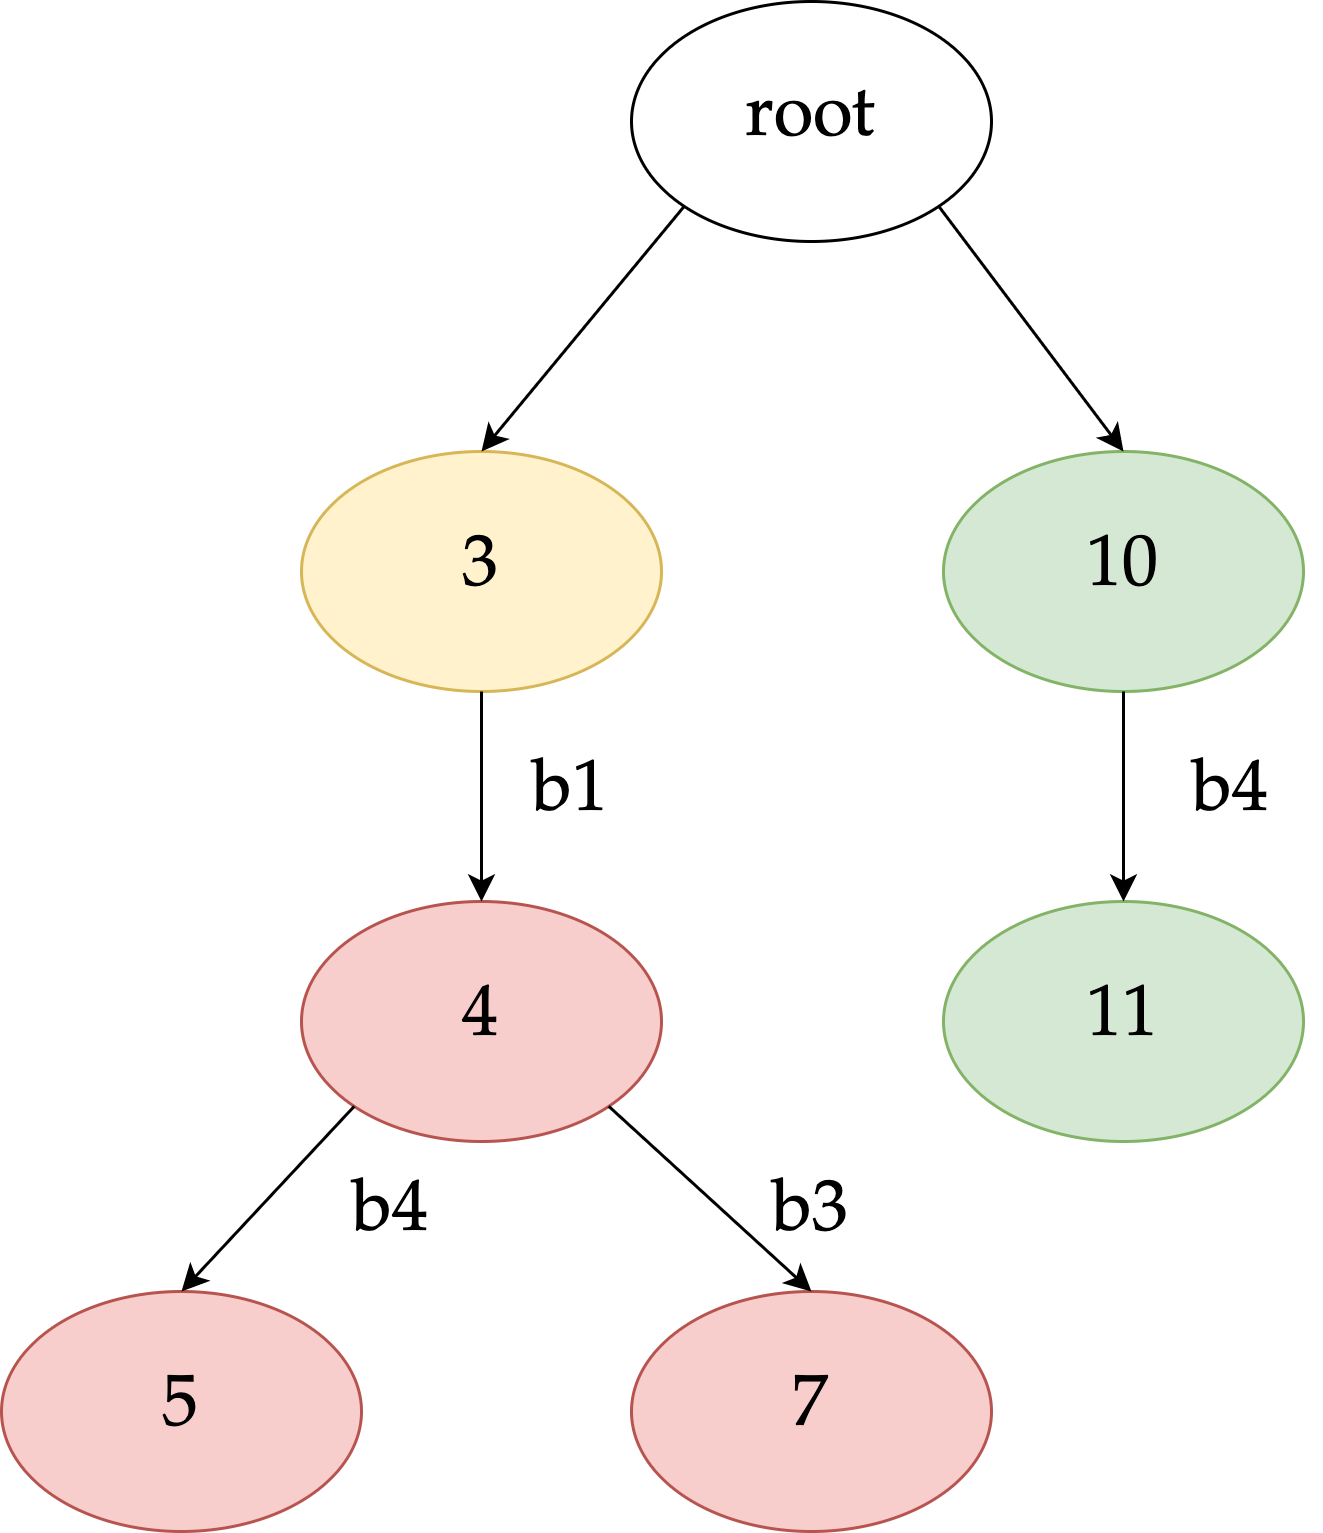
\includegraphics[width=0.5\textwidth]{cdg-code-example}
\label{fig:example-control-dependencies}
\end{figure}

%TODO DynaMOSA paper explains the terms dominator, post-dominator, dependence and so on.

Therefore, Panichella et al.~\cite{Panichella2018} introduced the \ac{DynaMOSA}, which adds to \ac{MOSA} the ability to dynamically focus the search on the subset of previously uncovered targets based on the control dependency hierarchy. The algorithm temporarily ignores uncovered targets that can only be reached by other uncovered targets placed higher in the dependency hierarchy. This is done because a population of test cases cannot cover ignored targets until their parents have been covered in the first place, which is attempted by the search focused only on the reachable parents and shall lead to a more effective consumption of the search budget. \Cref{fig:example-control-dependencies} shows the nodes of the control dependence graph that \ac{DynaMOSA} would consider with a given test \texttt{foo(1, 3, 3)}. Green marks the nodes covered by the test, yellow is the node that needs to be covered yet, and red nodes are temporarily ignored because the test cannot reach them at that point without covering nodes $3$ and $11$ first. Since \ac{DynaMOSA} optimizes a subset of the targets also considered by \ac{MOSA}, \ac{DynaMOSA} is guaranteed to be at least as efficient. In their experiments, the authors of both algorithms learned that \ac{DynaMOSA} achieved significantly higher coverage than \ac{WSA} and \ac{MOSA} on a dataset consisting of 346 Java classes.


\begin{algorithm}[t]
\caption{DynaMOSA Algorithm~\cite{Panichella2018}}\label{alg:dynamosa}
\begin{algorithmic}
\Input
  \Desc{$U$}{The set of coverage targets of a program}
  \Desc{$M$}{Population size}
  \EndInput
  \Output
  \Desc{$T$}{An evolved test suite}
  \EndOutput
\State $t \gets 0$
\State $P_t \gets RandomPopulation(M)$
\State $archive \gets UpdateArchive(P_t, \emptyset)$

\While{$\neg (search_budget_consumed)$}
    \State $Q_t \gets GenerateOffspring(P_t)$
    \State $archive \gets UpdateArchive(Q_t, archive)$
    \State $R_t \gets P_t \bigcup Q_t$
    \State $F \gets PreferenceSorting(R_t)$
    \State $P_{t + 1} \gets \emptyset$
    \State $d \gets 0$
    \While{$\left| P_{t + 1} \right| + \left| F_d \right| \leq M$}
        \State $CrowdingDistanceAssignment(F_d)$
        \State $P_{t + 1} \gets P_{t + 1} \bigcup F_d$
        \State $d \gets d + 1$
    \EndWhile
    \State $Sort(F_d)$
    \State $P_{t + 1} \gets P_{t + 1} \bigcup F_d[1 : (M - \left| P_{t + 1} \right|)]$
    \State $t \gets t +  1$
\EndWhile
\State $T \gets archive$
\State \Return $T$
\end{algorithmic}
\end{algorithm}

\begin{algorithm}[t]
\caption{$PreferenceSorting(T, M)$~\cite{Panichella2018}}\label{alg:preference-sorting}
\begin{algorithmic}
\Input
  \Desc{$T$}{A set of candidate test cases}
  \Desc{$M$}{Population size}
  \EndInput
  \Output
  \Desc{$F$}{Non-dominated ranking assignment}
  \EndOutput
\State $F_0 \gets \emptyset$
\For{$u_i \in U$ and $u_i$ is uncovered}
\State $t_{best} \gets \textrm{test case in T with minimum objective score for } u_i$
\State $F_0 \gets F_0 \bigcup \{t_{best}\}$
\EndFor

\State $T \gets T - F_0$
\If{$\left| F_0 \right| > M$}
\State $F_1 \gets T$
\Else
\State $U' \gets \{g \in U : u \textrm{ is uncovered}\}$
\State $E \gets FastNonDominatedSort(T, \{u \in U'\})$
\State $d \gets 0$
\For{All non-dominated fronts in $E$}
\State $F_{d + 1} \gets E_d$
\EndFor
\EndIf

\State \Return $F$
\end{algorithmic}
\end{algorithm}

\begin{algorithm}[t]
\caption{$UpdateArchive(T, A)$~\cite{Panichella2018}}\label{alg:update-archive}
\begin{algorithmic}
\Input
  \Desc{$T$}{A set of candidate test cases}
  \Desc{$A$}{An archive}
  \EndInput
  \Output
  \Desc{$A$}{An updated archive}
  \EndOutput
\For{$u_i \in U$}
\State $t_{best} \gets \emptyset$
\State $best\_length \gets \inf$
\If{$u_i$ already covered}
\State{$t_{best} \gets$ test case in $A$ covering $u_i$}
\State{$best\_length \gets$ number of statements in $t_{best}$}
\EndIf

\For{$t_j \in T$}
\State{$score \gets$ objective score of $t_j$ for target $u_i$}
\State{$length \gets$ number of statements in $t_j$}
\If{$score == 0$ and $length \leq best\_length$}
\State{replace $t_{best}$ with $t_j$ in $A$}
\State $t_{best} \gets t_j$
\State $best\_length \gets length$
\EndIf
\EndFor
\EndFor
\State \Return $F$
\end{algorithmic}
\end{algorithm}

\begin{algorithm}[t]
\caption{$CrowdingDistanceAssignment(T, M)$~\cite{Deb_2000}}\label{alg:crowding-distance-assignment}
\begin{algorithmic}
\Input
  \Desc{$T$}{A set of candidate test cases}
  \Desc{$M$}{A set of objectives}
\EndInput
\State{$l \gets \left|T\right|$}


\For{$i \in T$}
  \State{$T[i]_{distance} \gets 0$}
\EndFor

\For{$m \in M$}
  \State{$T \gets sort(I, m)$}
  \State{$T[1]_{distance} = I[l]_{distance} = \infty$}
  \For{$i = 2$ to $(l - 1)$}
    \State{$T[i]_{distance} \gets T[i]_{distance} + (T[i + 1].m - T[i - 1].m)$}
  \EndFor
\EndFor
\end{algorithmic}
\end{algorithm}

\section{Automatically Generated Oracles}
\label{sec:generated-oracles}
% TODO Teil davon ist Frasers Paper 1600 Bugs in 100 Projects
Traditionally, \ac{SBST} is applied to generate test suites that maximize some coverage criteria, e.g., branch coverage. However, search-based techniques usually do not employ automated oracles~\cite{Fraser2013}. A lack of formal specification of the behavior of a program results in generated tests that generally must be supplemented with oracles manually. Davis and Weyuker~\cite{10.1145/800175.809889} introduced the term \emph{non-testable programs}, which includes those programs which there is no test oracle for or a test oracle is impractical to implement. Thus one cannot check the result of the computation for correctness. This includes programs that were either created to learn the outcoming result in the first place, programs that give too many results to check them all, or the developer had misunderstood the specification. To solve the problem of missing oracles, the authors introduced the so-called pseudo oracle. A pseudo-oracle is a second, independently implemented program that must comply with the specifications. The two versions need to be created by separate teams with no intermediary communication so that no misunderstandings can propagate from one group to the other. Afterward, the results of the computations of the original program and the pseudo oracle can be compared, and a decision on validity can be made.

Hiring a second team of developers for this task is too time-consuming and expensive for most software. And so, there have been attempts to automate this process. Korel and Al-Yami~\cite{Korel1996} described an approach that uses search techniques to find violations of assertions in code. An assertion is simply a conditional whose \texttt{false} branch is assumed not to be executed. However, genetic or symbolic search can exploit the branch to look for a program state that violates the assertion explicitly. A violation leads in most programming languages to a program crash, which is the most basic variant of an automated oracle since an unexpected crash is a bad sign in most cases.

Romano et al.~\cite{Romano2011} proposed statically selecting possible paths that cause memory access violations and searching for inputs that direct execution into those paths. It is also possible to represent arithmetic errors such as division by zero as paths, so traditional \ac{SBST} metrics like branch distance can optimize the search for those errors~\cite{Bhattacharya2011}. Such techniques are called \emph{testability transformations} and were first (TODO \textbf{sicher?}) proposed by Harman et al.~\cite{Harman2004}. Those are often source-to-source transformations intended to improve the performance of various test generation algorithms. McMinn~\cite{McMinn2009} picked up the idea and proposed automatically generating pseudo-oracles for a given program. He applied testability transformations to modify the original program and develop a second version that is expected to have the same outputs as it's original but may have discrepancies. To this end, he provided two examples, floating-point arithmetic, and multithreading in Java. In the former, for instance, additions between primitive floating-point types, which are somewhat imprecise in the trailing decimal digits according to the IEEE standard~\cite{10.1145/103162.103163}, are swapped by Java's BigDecimal during a transformation, e.g., the calculation $0.1 + 0.1 + 0.1$ in Java yields ~$0.300000000000004$ instead of~$0.3$ (see~\Cref{lst:java-transformations}).

\begin{lstlisting}[language=Java, style=boxed, caption={Comparing floating-point arithmetic in Java using double compared to \texttt{BigDecimal}~\cite{McMinn2009}}, label=lst:java-transformations]
System.out.println(0.1 + 0.1 + 0.1);
// Output: 0.30000000000000004

System.out.println(
    new BigDecimal("0.1").add(
        new BigDecimal("0.1").add(
            new BigDecimal("0.1")
        )
    )
);
// Output: 0.3
\end{lstlisting}

McMinn applies transformations to serialize and deserialize a multithreaded program in their second example. Here, methods of a class are provided with Java's \texttt{synchronize} keyword; otherwise, the keyword is removed if a method is already synchronized. \texttt{synchronize} ensures that only one thread may use the respective method simultaneously. In their evaluation, the author tries to use the oracles generated by transforming the respective \sut for a genetic-based search for input data, maximizing the discrepancy between the outputs of the original program and its pseudo-oracle. This can detect potential bugs (discrepancy) and measure their severity (size of a discrepancy). Fraser and Arkuri~\cite{Fraser_2013} also took up the idea of automatically generating pseudo-oracles in their search-based test generator \textsc{EvoSuite}.

% TODO reword{}

Transformations have not only been applied in the context of search: the idea of checking error conditions was first mentioned in 1976 by Clarke~\cite{Clarke1976} in the context of symbolic execution. Active Property Checking~\cite{Godefroid_2005} describes usage of explicit error branches in the path constraints during \ac{DSE}. By having explicit constraints on the error conditions, \ac{DSE} exploration will try to negate also the error conditions, such that if there exists an input that leads to the error, it probably will be found. Other state-of-the-art \ac{DSE} tools also employ this approach, e.g., Pex~\cite{Tillmann2008} automatically adds constraints that check references against null, divisions against zero, etc. Barr et al.~\cite{Barr2013} instrument programs with additional branches to find floating-point exceptions with symbolic execution. These additional constraints are similar to the error conditions we introduce in the \mir transformation (see \Cref{sec:mir-testability-transformations}), even though some of them do not apply to Rust due to language peculiarities, e.g., there is no concept of null pointers in safe Rust.

\clearpage
\chapter{State of the Art}
\label{chap:state-of-the-art}
We give an overview of work related to ours in this chapter.

\section{Fuzzer for Rust}
% TODO reword
Fuzzing is a widely-adopted testing method that exercises a program by automatically generating inputs in a random or heuristic way. However, fuzzing approaches require defining fuzz targets. A fuzz target represents an array of bytes as input for executing a program composed of \acp{API} invocations~\cite{Jiang2021}. \ac{API} invocation chains are called fuzz drivers and usually need to be defined manually, too. Fuzzing tools can mutate the input of fuzz targets to explore different paths in \sut. \Cref{lst:fuzz-target-example} shows an example of a fuzz target for the example \sut \texttt{ex\_lib}.

\begin{lstlisting}[style=boxed, caption={A sample problem for fuzz target generation~\cite{Jiang2021}}, label=lst:fuzz-target-example]
mod ex_lib {
  struct S1;
  struct S2;
  fn f1(a: i16) -> S1;
  fn f2(b: u32) -> S2;
  fn f3(c: &[u8]) -> S2;
  fn f4(s1: S1, s2: &mut S2) -> S2;
  fn f5(s2: &S2, d: &str);
}

fn example_fuzz_target_1(data: &[u8]) {
  if data.len() > 3 {return;}
  let a = to_i16(data, 0);
  let c = to_slice::<u8>(data, 2, data.len());
  let s1 = ex_lib::f1(a);
  let mut s2 = ex_lib::f3(c);
  let _ = ex_lib::f4(s1, &mut s2);
}
\end{lstlisting}

\textbf{AFL++} is a reengineered fork of the popular coverage-guided fuzzer \textsc{AFL} by Zalewski~\cite{Zalewski2014}. It is an extensible community-driven open-source tool that incorporates state-of-the-art fuzzing research. The tool mutates a set of test cases to reach previously unexplored points in the program. The test case triggering new coverage is saved as part of the test case queue~\cite{Fioraldi2020}. Researchers can easily extend the current implementation with additional techniques and use the tool as a baseline for evaluating new ideas. \emph{afl.rs} provides the ability to apply \textsc{AFL++} to Rust.

\textbf{LLVM libFuzzer} is another coverage-guided evolutionary fuzzing engine . It feeds fuzzed inputs to the library under test via specific fuzzing entry points, also known as \emph{target functions}. The fuzzer tracks which areas of the code are reached and generates mutations on the corpus of input data to maximize the coverage. Some other tools build upon the \textsc{libFuzzer} and extend it with techniques like concolic testing~\cite{Rocha2020,Le2019}. Both LLVM libFuzzer and \textsc{AFL++} require manually written fuzz targets, however, i.e., a chain of invocations and a recipe where to put the generated data.

\textsc{RULF} is a fuzz target generator that, given the \ac{API} specification of a Rust library, can generate a set of fuzz targets and seamlessly integrate them with \textsc{AFL++} for fuzzing~\cite{Jiang2021}. The approach leverages a sophisticated traversal algorithm to achieve high \ac{API} coverage with only a tiny set of shallow fuzz targets. To construct fuzz targets, the tool builds an \ac{API} dependence graph and analyses which \ac{API} calls return values of the type used as a parameter for other \ac{API} calls of the same \sut. Using their approach, the authors discovered several bugs in popular Rust libraries. An essential limitation of the tool is its inability to analyze and fuzz generic components.

\section{DSE-based Test Generators}
Many tools rely on \ac{DSE} for the automatic generation of tests, for example \textsc{CUTE}, \textsc{jCUTE}~\cite{Sen2006}, and \textsc{KLEE}~\cite{cadar2008klee}. \textsc{KLEE} has two goals: (1) the tool tries to execute every executable line in a program, i.e., to achieve high statement coverage, and (2) for every dangerous operation (e.g., dereference, assertion), it tries to check whether there are values that could lead to an error. The latter is achieved by symbolic execution. Since, even in simple programs, the number of execution states/paths can explode, \textsc{KLEE} applies several heuristics and optimization techniques to increase its performance. For example, whole trees are not cloned at branches (states are trees, after all), but the write-on-copy approach is applied at the object level. Several different states can reference unchanged subtrees. Also, requests to the \ac{SMT} solver to convert symbolic values to concrete ones are simplified as possible since the processing time of the requests, which generally are NP-complete~\cite{Lewis1983}, dominates everything else. In this way, the authors were able to speed up the execution time of the tool on the GNU coreutils by a factor of $15$.

\textbf{DART}~\cite{Godefroid_2005} was the first concolic testing tool that combined dynamic test generation with random testing and model checking techniques to systematically execute as many as possible feasible paths of a program while checking each execution for various types of errors.


\textbf{CUTE} (Concolic Unit Testing Engine) and \textbf{\textsc{jCUTE}} (CUTE for Java)~\cite{Sen2006} are also two tools that can generate minimal tests, including input data for C as well as Java programs using \ac{DSE} respectively. The tools extend \textsc{DART} and generate random input data to initiate search and progress when symbolic execution fails to progress due to the limitations mentioned before. In addition, multithreaded programs are handled that manipulate dynamic data structures using pointer operations. \textsc{CUTE} combines concolic execution with dynamic partial order reduction in multithreaded programs to generate both test inputs and thread schedules systematically. \textsc{CUTE} discoverd some actual bugs during the evaluation with popular open-source libraries and Java Standard Library.


\textbf{KLEE} redesigns its predecessor \textsc{EXE}~\cite{Cadar2008} and is built on top of LLVM compiler infrastructure. It uses the \ac{IR} emitted during compilation. The tool performs mixed concrete/symbolic execution, models memory with bit-level accuracy, employs a variety of constraint solving optimization, and uses search heuristics to get high code coverage. In addition, for each dangerous operation (e.g., dereference, assertion), the tool tries to check whether there are values that could lead to an error in the process. In the experiments, the tool generated tests that exceeded the coverage of manually written tests and could find bugs even in such commonly used and heavily used tools as parts of the GNU Coreutils. Since, even in simple programs, the number of execution states/paths can explode, \textsc{KLEE} applies multiple heuristics and optimization techniques to improve performance. For instance, whole trees are not cloned at decision branches (states are, after all, trees). Instead, the write-on-copy approach is applied at the object level. Several different states can reference unchanged subtrees.

Moreover, requests to the \ac{SMT} solver to convert symbolic values into concrete ones are attempted to be as simplified as possible since the requests' processing time dominates everything else. In this way, the authors were able to speed up the execution time of the tool on the GNU Coreutils by 15 times. With the birth of Rust, it was later possible to apply KLEE to the LLVM IR of the Rust compiler.

The authors of \textsc{KLOVER}~\cite{Li2011} describe the tool as the first to allow symbolic execution and test generation for industrial C++ programs. It builds on top of \textsc{KLEE}, works with the LLVM bitcode, and extends \textsc{KLEE}'s optimizations to C++ language features, for example, classes and objects and LLVM intrinsics.


\section{Search-based Test Generators}
\textbf{EvoSuite}~\cite{Fraser_2011} is a tool that automates the task of generating unit tests by systematically producing test suites that achieve high coverage, are as small as possible, and provide assertions. \textsc{EvoSuite} uses not only a search-based approach but also exploits \ac{DSE}, hybrid search, and testability transformations~\cite{Harman2004} to improve its efficiency. The tool targets programs with no formal specification, which could be used to derive oracles to test the actual behavior against the expected one. However, it uses mutation testing to produce a reduced set of assertions. The assertions highlight the relevant aspects of the current behavior to support developers in identifying defects. \textsc{EvoSuite} used to apply the \ac{WS} approach but has employed other \acp{GA} ever since, too, e.g., \ac{DynaMOSA}. The tool sets the bar for the quality of automatically generated tests~\cite{Vogl2021,Panichella2020,Campos2019,Fraser2018,Fraser2016,Fraser2017}.

\textbf{SUSHI}~\cite{Braione2018} is an open-source test generator for Java that combines both concolic and evolutionary testing. It does the latter by leveraging \textsc{EvoSuite}. The tool tries to synthesize test suites with high branch coverage. It explores the program execution space and computes the execution conditions of the program paths. Afterward, the path conditions will be translated into executable evaluators that quantify the distance of a concrete state from satisfying the corresponding path condition.

\textbf{EvoObj}~\cite{Lin2021} is an extension to \textsc{EvoSuite}. The tool tackles the problem that the effectiveness of \ac{SBST} suffers greatly when generating complex object inputs due to search spaces that are neither continuous nor monotonic. \textsc{EvoObj} employs analysis of static control and data flow of a \sut to create \emph{seed tests}. The seed tests can drastically increase the performance of the search by providing a more continuous and monotonic fitness landscape.

\section{Random Testing Tools}
\textbf{Randoop}~\cite{Pacheco_2007} generates unit tests for Java code using feedback-directed random test generation. Feedback-directed random testing uses execution feedback gathered from executing test inputs as they are created to avoid generating redundant and illegal inputs. Randoop can verify some basic assumptions on programs. For instance, programs should not crash, which is a sort of automated oracle. The tool can also check  contracts on the code, which the user may supply. By default, it implements multiple default contracts that the Java language employs, e.g., reflexivity of \emph{Object.equals}~\cite{Fraser2013}. Randoop outputs two test suites; one contains contract-violating tests. The other has \emph{regression} tests, which do not violate contracts but instead capture an aspect of the current implementation of a \sut. Those can discover inconsistencies between two versions of a program.


\clearpage
\chapter{Rust Programing Language}
\label{chap:rust-programming-language}
% TODO das sollte natürlich umformuliert werden
Rust is an increasingly popular programming language designed to be fast, efficient, and safe. The design of the language began in 2006, while the first stable version was released in 2015. The high-level goal of the language is performance comparable to systems programming languages like C and C++ without sacrificing the safety of higher-level languages, e.g., like Java and Python.

This is a challenging problem to solve because system programming languages need to be able to control how memory is managed explicitly to be performant, which is easy for a langugage user to do incorrectly. The higher-level languages sacrifice this control for convenience, using tools such as garbage collectors to automate memory management. Consider, as an example, how C and Java handle heap memory. In C we can allocate memory on the heap by using the \texttt{malloc} or \texttt{calloc} functions. The data on the heap can then be reclaimed with \texttt{free}. These functions are easily misused, e.g., by calling free twice on the same pointer, which leads to undefined behavior, and forgetting to free memory would be wasting that memory. Java, and many other high-level programming languages, use a different approach. A programmer does not have to allocate and deallocate heap memory manually; the garbage collector reclaims it at runtime now and then based on heuristics. While this makes writing programs that correctly handle memory easier, it also impacts the execution performance due to the operational overhead of determining which memory is no longer in use and freeing it.

Rust addresses this issue by the ownership system, which requires a developer to write code the way that the compiler can infer when exactly memory should be allocated and released. If the code does not satisfy the requirements, it will not compile.

\section{Tooling}
Rust comes with official package managers, which we briefly describe in the following sections.

\subsection{Cargo}
Cargo is the name of Rust's package manager and build system, which is provided out-of-the-box. It can create new packages, download dependencies, and compile packages. It also supports more advanced features like publishing packages and running tests. Packages created and used by Cargo are known as crates. Cargo is designed to be the central tool that developers use when working with crates.

\subsection{Rustup}
While Cargo is used to manage crates, Rustup is used to manage Rust tools, like Cargo and the Rust compiler flavors, and any other components which have been added to the toolchain. Among other things, Rustup makes it possible to have fine-grained control over the version of Rust used to compile crates. To understand how this affects development, we explain the versioning used in the Rust ecosystem. New stable and beta versions of Rust are released every six weeks, and a nightly version is released every night, based on the previous day's main branch in the central git repository. The beta versions are based on the latest nightly every six weeks, and the stable versions are based on the previous beta.
Features introduced in nightly versions of the compiler must be explicitly enabled in the source code, as shown in \Cref{lst:example-enable-feature}.

\begin{lstlisting}[style=boxed, caption=Enabling features in Rust, label=lst:example-enable-feature]
#![features(box_patterns)]
\end{lstlisting}

To develop any sort of tooling for Rust, developers must use nightly versions, although they can pin the version to a specific date if they wish.
Rustup allows developers to set the version specifically for a given project or a global default.

\section{Language Basics}
The Rust language itself is unique in many ways, and we strive to summarize the key points in the following subsections.

\subsection{Syntax}
Rust syntax is mostly in line with the C family of languages. The ubiquitous Hello, World! program can be written as shown in \Cref{lst:example-hello-world}.
\begin{lstlisting}[style=boxed, caption=Hello World, label=lst:example-hello-world]
println!("Hello World!");
\end{lstlisting}

In \Cref{lst:example-struct-enum}, we demonstrate a struct and an enum type definition with generics. The angle brackets indicate the generics and, in this case, those are two anonymous type parameters. Enums and structs are the two main types available in Rust. Enums are most often accessed via pattern matching, whereas struct fields can be accessed directly. While curly brackets indicate scope and statements end with a semicolon, Rust differs from the C family of languages in regerd of its function definitions, which do not start with the return type. Typically, the types are written after the identifiers, as demonstrated in \Cref{lst:example-functions-struct-enum}.

\begin{lstlisting}[style=boxed, caption={The type definition for a point in two-dimensional space and an enum definition}, label=lst:example-struct-enum]
struct Point {
  x: f64,
  y: f64
}

enum Result<T, E> {
  Ok(T),
  Err(E)
}
\end{lstlisting}

In \Cref{lst:example-functions-struct-enum}, we compute and return a new point, placed in between the two points provided. This may look strange to those used to seeing the return keyword used instead. While it is possible to return values in that way, it is considered idiomatic Rust to return by ending the function with an expression, which the compiler implicitly interpretes as a return statement.

\begin{lstlisting}[style=boxed, caption={A function to compute the point between two points in two-dimensional space}, label=lst:example-functions-struct-enum]
fn middle(p1: Point, p2: Point) -> Point {
  Point {
    x: (p1.x + p2.x) / 2,
    y: (p1.y + p2.y) / 2
  }
}
\end{lstlisting}

Structs do not have explit constructors as other languages do for classes. However, it is a convention to provide a static method called \texttt{new} that instantiates a struct.

\subsection{Associated Functions and Methods}
Functions can be associated with types in Rust, e.g., with enums or structs. Rust separates the definition of behavior from the definition of data. To implement behavior for an enum or a struct, we can add an \texttt{impl} block, as shown in \Cref{lst:example-associated-function}. An example of a common associated function is \texttt{new} which returns a value of the type it is associated with.

\begin{lstlisting}[style=boxed, caption={Associating behavior with the \texttt{Point} data type defined in \Cref{lst:example-struct-enum}}, label=lst:example-associated-function]
impl Point {
  fn new(x: f64, y: f64) -> Self {
    Self { x, y }
  }
}

let p = Point::new(32.0f32, 42.0f32);
\end{lstlisting}

Associated functions whose first parameter is named \texttt{self} are called methods and may be invoked using the method call parameter, for instance, \texttt{x.foo()}, as well as the usual function call annotation. \texttt{self} is an instance of the type \texttt{Self}, which, in the scope of a struct, enum, or trait, is an alias for the enclosing type. Through \texttt{self}, we can access the state and methods of the instance, e.g., as in \Cref{lst:example-method}.

\begin{lstlisting}[style=boxed, caption={Defining a method on \texttt{Point} data type from \Cref{lst:example-struct-enum}}, label=lst:example-method]
impl Point {
  fn new(x: f64, y: f64) -> Self {
    Self { x, y }
  }

  fn add(&self, other: &Self) -> Self {
    Self {
      x: self.x + other.x,
      y: self.y + other.y
    }
  }
}

let p1 = Point::new(32.0f64, 42.0f64);
let p2 = Point::new(10.0f64, 10.0f64);

let result = p1.add(&p2);

// Syntactical sugar for

let result2 = Point::add(&p1, &p2);
\end{lstlisting}


\subsection{Traits}
A trait describes an abstract interface that types can implement. This interface consists of associated items, which come in three variants: functions, associated types, constants. Traits are implemented for specific types through separate \texttt{impl} blocks. Trais functions can have default implementations, which implementing types can exploit if they do not provide custom implementations. Otherwise, an unimplemented trait's function body indicates that the implementor must override it. Similarly, associated constants may omit the equals sign and expression to indicate implementations must define the constant value. Associated types must never define the type; the type may only be specified in an implementation. As an example, a trait could be defined for implementing a method that generates a string from an instance of a type, as shown in \Cref{lst:example-trait}.

\begin{lstlisting}[style=boxed, caption={Trait definition and implementation for the \texttt{Point} data type from \Cref{lst:example-struct-enum}}, label=lst:example-trait]
trait ToString {
  fn to_string(&self) -> String;
}

impl ToString for Point {
  fn to_string(&self) -> String {
    format!("({}, {})", self.x, self.y)
  }
}

let p = Point::new(32.0f64, 42.0f64);
let textual_repr = p.to_string();
\end{lstlisting}

% When the associated function is declared on a trait, the function can also be called with a path that is a path to the trait appended by the name of the trait. When this happens, it is substituted for \texttt{<_ as Trait>::function_name}.

\subsection{Generics and Trait Objects}
% TODO reword
Rust supports generic types and allows for shared behavior via traits. Generics parametrize data structures, methods, and functions, such that different types can reuse same code. This improves usability and helps finding type errors statically. The language provides static and dynamic dispatch. The former is realized by means of monomorphization, i.e., for each type a generic implementation is used with, the compiler generates a concrete implementation of it and replaces the call sites with calls to the specialized functions. As a consequence, the final binary will be slightly larger due to potentially many copies of the same code, but calling the functions will not result in any runtime dispatch overhead. Moreover, due to static type information, the compiler can inline the code, which generally leads to better performance. \Cref{lst:static-dispatch} demonstrates a generic data type that uses static dispatch.

\begin{lstlisting}[style=boxed, caption={A data type with static dispatch via monomorphization}, label=lst:static-dispatch]
struct Pair<L, R> {
  left: L,
  right: R
}

impl<L, R> Pair<L, R> {
  pub fn of(left: L, right: R) -> Self {
    Pair { left, right }
  }

  pub fn left(&self) -> &L {
    &self.left
  }

  pub fn right(&self) -> &R {
    &self.right
  }
}
\end{lstlisting}

% TODO reword
With dynamic dispatch, trait objects come into play. Those are usual instances of any type that implements the given trait, where the precise type can only be known at runtime. The methods of the trait can be called on a trait object via the \emph{vtable}, which is created an managed by the compiler. A function that takes trait objects is not specialized to each type that implements the trait: only one copy of the code is generated, resulting in less code bloat. However, this comes at the cost of requiring slower virtual function calls and effectively inhibiting any chance of inlining and related optimizations from occurring. When using trait objects, they must be packed into a data type with a known compile-time size, e.g., a \texttt{Box}, which is a pointer into the heap, as demonstrated in \Cref{lst:dynamic-dispatch}.

\begin{lstlisting}[style=boxed, caption=A data type with dynamic dispatch, label=lst:dynamic-dispatch]
struct Pair {
  left: Box<dyn Any>,
  right: Box<dyn Any>
}


impl Pair {
  pub fn of(left: Box<dyn Any>, right: Box<dyn Any>)
    -> Self {
    Pair { left, right }
  }

  pub fn left(&self) -> &Box<dyn Any> {
    &self.left
  }

  pub fn right(&self) -> &Box<dyn Any> {
    &self.right
  }
}
\end{lstlisting}

With the definition from \Cref{lst:static-dispatch}, we can now create \texttt{Pair} instances with different types as shown in \Cref{lst:example-generics-usage} using monomorphization, e.g., \texttt{String} and \texttt{u32} or two times \texttt{usize}. The same code is reused, and the compiler can statically check whether the a pair instance uses values of correct type:
\begin{lstlisting}[style=boxed, caption={}, label=lst:example-generics-usage]
fn main() {
  let pair: Pair<String, u32> = Pair::of(
    "Hello world".to_string(), 42u32
  );
  let left_value: &str = pair.left();

  let another_pair: Pair<usize, usize> = Pair::of(
    0usize, 1usize
  );
}
\end{lstlisting}
TODO The compiler can now extract the relevant types and generate the following code

It is also possible to put constraints, called trait bounds in Rust, on the generic type parameters. For instance, we could define a textual representation of a pair. The \texttt{Display} trait of the standard library provides the \texttt{fmt} method, which uses the \texttt{\string{\string}} print marker. As shown in \Cref{lst:example-trait-bounds}, for a type to implement the \texttt{Display} trait, its attributes must implement the trait, too, since their \texttt{fmt} method will be called recursively. Hence, we tell that the left and right hand side type parameters used with the \texttt{Pair} struct must implement the \texttt{Display} trait. The effect of bounding is that generic instances are allowed to access the methods of traits specified in the bounds. Under the hood, the \texttt{println!} macro call the \texttt{fmt} method of the \texttt{Pair} instance:
\begin{lstlisting}[style=boxed, caption={}, label=lst:example-trait-bounds, escapechar=§]
struct Pair<L: Display, R: Display> {
    left: L,
    right: R
}

impl<L: Display, R: Display> Pair<L, R> {
  pub fn of(left: L, right: R) -> Self {
    Pair { left, right }
  }
}

impl<L: Display, R: Display> Display for Pair<L, R> {
  fn fmt(&self, f: &mut std::fmt::Formatter)
      -> std::fmt::Result {
    write!(f, "({}, {})", self.left, self.right)
  }
}

fn main() {
  let pair: Pair<String, u32> = Pair::of(
    "Hello world".to_string(), 42u32 §\label{line:example-trait-bounds:str-type-conversion}§
  );
  println!("{}", pair);
  // Output: (Hello world, 42)
}
\end{lstlisting}

We need to convert \texttt{"Hello world"} TODO

There is no inheritance in Rust, as known from object-oriented languages. Common behavior can be defined via traits, which can have super-traits, as shown in \Cref{lst:trying-supertraits} for the \texttt{TrieAtom} trait. \texttt{TrieAtom} is a blanket trait, which means that types that implement its super trait automatically implement it, too, from the compiler's point of view.
\begin{lstlisting}[style=boxed, caption={An example trait from the \emph{trying} crate which we evaluate the approach on}, label=lst:trying-supertraits]
pub trait TrieAtom: Copy + Default + PartialEq + Ord {}
\end{lstlisting}

Besides structs, it is also possible to parametrize methods and functions using generics. A generic method or function has a type parameter that is inferred from the values passed as parameters. TODO An example for
\begin{lstlisting}[style=boxed, caption={Variants of defining a generic function}, label=lst:function-monomorphization]
fn make_pair<L: Display, R: Display>(left: L, right: R)
    -> Pair<L, R> {
  Pair::of(left, right)
}

// Alternative syntax for monomorphism,
// useful when the definition grows large
fn make_pair<L, R>(left: L, right: R) -> Pair<L, R>
where L: Display, R: Display {
  Pair::of(left, right)
}

fn main() {
  let pair: Pair<String, String> = make_pair(
    "Hello".to_string(),
    "world".to_string()
  );
  let another_pair: Pair<usize, u32> = make_pair(
    4usize, 2u32
  );
}
\end{lstlisting}

The function \texttt{make\string_pair} creates a generic \texttt{Pair} instance. Then, it is used again to create a pair of two strings and a pair of a \texttt{usize} and a \texttt{u32}.

Traits may also contain additional type parameters. Other traits may constrain these type parameters and so on; see \Cref{lst:traits-with-type-bounds}. Usually, the more constraints, the more difficult it is to find correct types and automatically generate test cases that use those features and do compile.

\begin{lstlisting}[style=boxed, caption={Type parameters can be specified for a trait to make it generic. These appear after the trait name, using the same syntax used in generic functions}, label=lst:traits-with-type-bounds]
trait PrintableSeq<T: Display> {
  fn len(&self) -> usize;
  fn at(&self, pos: usize) -> T;
  fn iter<F>(&self, f: F) -> where F: Fn(T);
}
\end{lstlisting}

\subsection{Ownership and Borrowing}
As mentioned at the beginning of the chapter, Rust's approach to memory management is different from the traditional one of C or C++, where memory is managed manually through functions like \texttt{malloc} and \texttt{free}, or by letting the garbage collector manage the resources. In Rust, each value has a variable that's called its owner. There can only be one owner of a value at a time, and once the owner goes out of scope, the value is deallocated.

\begin{lstlisting}[style=boxed, caption=Heap data owned by binding, label=lst:example-ownership]
{
  // The String data on the heap is created
  // and set to be owned by binding a
  let a = String::from("content");
}
// The scope in which a is active is over,
// and a is now no longer valid. At the same
// time the string data on the heap is freed
\end{lstlisting}

In cases where the value needs to outlive a given scope, it can be moved to a new owner in a different scope. This happens, for example, when a value is passed as a parameter to a function, or on assignment, with the caveat that some values are so cheaply copied that a move is never necessary.

\begin{lstlisting}[style=boxed, caption=Transferring Ownership, label=lst:transfer-ownership]
let b;
{
    let a = String::from("content");
    b = a;

    println!("The content is: {}", a);
    // Trying to use a after transferring the
    // ownership results in a compilation error
}
\end{lstlisting}

Moving values would quickly become burdensome when we want to reuse a value, e.g., after passing it to a function invocation. In Rust, we can also reference variables. References can be immutable (read-only) or mutable, meaning that the reference owner has write access to the underlying value. Creating a reference is also known as borrowing in Rust, a fundamental interaction aspect in the ownership model. The reference owner cannot modify the value by default when borrowing a value. It can only be borrowed mutably if it is not referenced somewhere else for the duration of the borrow. On the other hand, a value can be borrowed immutably multiple times, as there is no possibility of a race condition when the underlying cannot be modified.

These rules make it possible for the compiler to infer when resources can be deallocated, guarantee memory safety, and make it impossible to create structures that are not tree-formed without an additional level of indirection. For example, implementing a linked list with these restrictions would be impossible since a list node is a recursive data structure. That is because the ownership system is an over-approximation of memory safety; sometimes, the compiler can reject completely valid and safe code. This is why some parts of the standard library is implemented using the \texttt{unsafe} keyword, which allows the programmer, among other things, to bypass these rules. In practice, this means that memory bugs still happen in Rust but the ownership system prevents them from originating in safe Rust.

%TODO Ownership spielt auch für die generierten Tests eine wichtige Rolle und macht die Generierung schwieriger, als zum Beispiel in Sprachen wie Java. Das ist zum Beispiel aus \Cref{lst:ownership-method-call} ersichtlich.
\begin{lstlisting}[style=boxed, caption={Transferring the ownership to a method}, label=lst:ownership-method-call]
fn main() {
    let mut message = String::from("Hello");
    print(message); // Value moved here
    // Compile error, value borrowed here after move
    message.push_str(" world!");
}

fn print(message: String) {
  // message gets dropped when the execution
  // goes out of scope
  println!("{}", message);
}
\end{lstlisting}

The problem with the ownership model described above is that if we want to continue working with the moved value after a function call, such as in \Cref{lst:ownership-method-call}, the called function must return the value to the calling function since, in the example, the string moved into the function \texttt{print}. Instead, we can pass a reference to the value as an argument to the invoked function, which is like a pointer to the value, so the function can follow the address and access the value. Unlike a pointer in C, a reference in safe Rust is guaranteed to point to the correct memory. As shown in \Cref{lst:borrowing-method-call}, a reference to a value can be passed using \texttt{\string&}. The syntax \texttt{\string&message} provides the ability to reference the string value, i.e., borrow it. Since the reference does not own the value, the actual value will not be deallocated when the reference is no longer alive.

\begin{lstlisting}[style=boxed, caption={Transferring the ownership to a method}, label=lst:borrowing-method-call]
fn main() {
    let mut message = String::from("Hello");
    // A reference to message
    // it passed to the function call
    print(&message);
    // Variable message still owns the value
    // after the call
    message.push_str(" world!");
}

// The function borrows the value of message
fn print(message: &String) {
  println!("{}", message);
}
\end{lstlisting}

Whether owned or borrowed, values cannot be changed by default, as this is prevented by the compiler. If this is still necessary, it must be explicitly specified with the keyword \texttt{mut}, as in \Cref{lst:mut-borrowing-method-call}.

\begin{lstlisting}[style=boxed, caption=Transferring the ownership to a method, label=lst:mut-borrowing-method-call]
fn main() {
    let mut text = String::from("Hello");
    extend_msg(&mut text);
    println!("{}", &text);
    // Output: Hello world!
}

fn extend_text(text: &mut String) {
    text.push_str(" world!");
}
\end{lstlisting}

Thus, the restrictive ownership model has particular implications for the generated tests, i.e., we cannot use variables arbitrarily and need to observe their ownership state.

\section{Overview of the Compiler}
As with most compilers, the Rust compiler (\emph{rustc}) goes through several phases, using multiple \acp{IR} to facilitate computations. Working directly with the source code is highly inconvenient and error-prone. Source code is designed to be human-friendly while at the same time being unambiguous, but it's less convenient for analysis, e.g., type checking.

Instead, most compilers, including \emph{rustc}, build some \acp{IR} out of the source code, which is easier to process. rustc has a few \acp{IR}, each optimized for different purposes:

\begin{itemize}
    \item Token stream: the lexer produces a stream of tokens directly from the source code. This stream is easier for the parser to deal with than raw text.
    \item \ac{AST}: the abstract syntax tree is built from the stream of tokens. It represents almost exactly what a user wrote. It helps to do some syntactic sanity checking (e.g., checking that a type is expected where the user wrote one).
    \item \hir: This is a desugared and compiler-friendly representation of the \ac{AST} that is generated after parsing, macro expansion, and name resolution. It is still close to what the user wrote syntactically, but it includes implicit information such as elided lifetimes. Also, some expression forms have been converted to simpler ones, e.g., \texttt{for} loops are converted to a more basic \texttt{loop}. This \ac{IR} is amenable to type checking.
    % Lowering to HIR: https://rustc-dev-guide.rust-lang.org/lowering.html
    \item \ac{THIR}: This is an intermediate between \hir and \mir. It's similar to \hir but it is fully typed and a bit more desugared.
    \item \mir: This \ac{IR} is a \cfg. It shows the basic blocks of a program and how control flow connects them. A basic block contains simple typed statements (e.g., assignments, primitive computations, etc.) and control flow pointers to other basic blocks. This representation is used for borrow checking and other important data flow-based checks, such as exposing uninitialized values.
    \item LLVM \ac{IR}: This is a standard form of all input to the LLVM compiler. LLVM \ac{IR} is a typed assembly language with lots of annotations. It is designed to be easy for other compilers to emit and rich enough for LLVM to run optimizations.
\end{itemize}

\subsection{High-Level Intermediate Representation}
%TODO
Many parts of the \hir resemble Rust surface syntax quite closely, with the exception that some of Rust's expression forms have been desugared away.

%Für die Analyse von verfügbaren Strukturen, Methoden und Funktionen müssen wir möglichst viele Informationen bekommen, die vom Compiler zur Verfügung gestellt werden. Die \hir ist dafür perfekt geeignet, denn auf dieser Ebene werden zugleich die Typen explizit vom Compiler ausgefüllt und es werden noch alle für uns relevante Sprachelemente beibehalten. Lediglich werden intraprozedurale Elemente desugared,
For the analysis of available structures, methods and functions we need to get as much information as possible, which is provided by the compiler. The \hir is perfectly suitable for this purpose because the compiler fills implicit type information but all the representation still keeps all language elements that are relevant for us. Only intraprocedural elements are desugared, for instance, \texttt{for} loops are converted into a \texttt{loop} and do not appear in the \hir.
\begin{lstlisting}[style=boxed, caption={An example Rust program that we convert to HIR}, label=lst:hir-lowering]
struct IntVec {
    vec: Vec<i32>
}

impl IntVec {
    pub fn foo(&mut self) {
        for n in self.vec {
            // Does something
        }
    }
}
\end{lstlisting}

\Cref{lst:hir-lowering,lst:hir-lowered} compare an example program representation before and after lowering to \hir. The main differences are the desugared \texttt{for} loop and the filled-in type declaration of the \texttt{self} parameter of the \texttt{foo} method. TODO Da wir für das Generieren eines Tests für die gegebene \texttt{foo} Methode nur die Methodensignatur sowie die Structdefinition brauchen, stellt das Desugaring kein Problem dar.

\begin{lstlisting}[style=boxed, caption={HIR of the code in \Cref{lst:hir-lowering}}, label=lst:hir-lowered]
struct IntVec {
    vec: Vec<i32>,
}

impl IntVec {
  pub fn foo(self: &mut Self) -> () {
    {
      let _t = match #[lang = "into_iter"](self.vec) {
        mut iter => loop {
          match #[lang = "next"](&mut iter) {
            #[lang = "None"] {} => break,
            #[lang = "Some"] { 0: n } => {
              {
                // Does something
              };
            }
          }
        },
      };
      _t
    }
  }
}
\end{lstlisting}

The next lowering step, i.e., \ac{THIR}, similarly to \mir, only contains function bodies, i.e., executable code. Consequently, \ac{THIR} has no representation for items such as \texttt{struct} or \texttt{trait} and is therefore not suitable for this type of analysis.

\subsection{Mid-Level Intermediate Representation}
% TODO umformulieren und so
\mir is based on the \cfg of a function body and is fully typed. The \mir for a given function body consists of a series of basic blocks. A basic block is an atomic unit of the program's \cfg, is guaranteed to execute entirely, and is made up of a sequence of statements followed, optionally, by a terminator, which corresponds to an edge in the \cfg. Being very much internal to the Rust compiler, \mir does not have a stable definition and undergoes frequent changes. There is no stable surface syntax for \mir, only one intended for debugging, which we will use here to show examples of analysis and instrumentation. Instead, it is defined as a collection of data structures. \mir has enough information to make our program instrumentation feasible, though its unstable nature makes the consumption of \mir challenging to maintain across different toolchain versions.

At this level, each executable piece of code, e.g., a function or a method, is represented as a \texttt{Body} object, which contains information about locals (parameters, user-defined variables, compiler-defined variables, and the return value) and basic blocks.

Locals are memory allocations on the stack (conceptually, at least), such as function arguments, local variables, and temporaries. These are identified by an index, written with a leading underscore, like \texttt{\string_1}. A special local (\texttt{\string_0}) is allocated to store the return value.

Basic blocks consist of statements, which are, in terms of \mir, actions with one successor. The statements of a basic block are mostly definitions of locals, e.g., atomic computations, which the corresponding terminator uses later. A terminator is an action with potentially multiple successors and is always placed at the end of a basic block. A terminator can be, for instance, a \emph{Call} (function call), a \emph{Return} (returns the \texttt{\string_0} local), a \emph{Goto} jump (jump to a given block number), a \emph{SwitchInt}, or an \emph{Assert}. \tech makes use mainly of \emph{SwitchInt} and \emph{Assert} terminators.

\emph{SwitchInt} results from lowering \texttt{if} and \texttt{loop} conditions and \texttt{match} expressions. The value of its operand always evaluates to an integer; the execution jumps depending on its value to one of the targets. There is also a dedicated \emph{otherwise} value for all other cases. Each possible value (e.g., $0$ and $1$ for \emph{false} and \emph{true}, respectively, in if conditions) has a corresponding basic block which the execution jumps to. Assume that there are two functions, \texttt{cheeky\string_itoa(x: i32)} and \texttt{bold\string_itoa(x: i32)}, which both return a string (more precisely, a reference to a static string value) based on the input number, as shown in~\Cref{lst:mir-lowering}.

\begin{lstlisting}[style=boxed, caption={HIR of the code in \Cref{lst:hir-lowering}}, label=lst:mir-lowering]
fn cheeky_itoa(x: i32) -> &'static str {
  match x {
    0 => "There is nothing here,
      only the infinite emptiness",
    42 => "The answer to everything",
    _ => "Must be some huge value"
  }
}

fn bold_itoa(x: i32) -> &'static str {
  if x > 42 {
    "Must be some huge number"
  } else {
    "Not that huge, I'd say"
  }
}
\end{lstlisting}

As mentioned earlier, conditions like those in loops, \texttt{match} and \texttt{if} expressions are converted to \texttt{switchInt} terminators. In \Cref{lst:mir-lowered-first}, the \mir for the function \texttt{cheeky\string_itoa} is shown in its debug form. It has been cleaned up for simplicity and usually still includes many debugging comments on the individual statements and terminators. Only two locals are given, the return value \texttt{\string_0} of type \texttt{\string&str}
and the function parameter \texttt{\string_1} of type \texttt{i32}.

We can see that the entry block, which is always \texttt{bb0}, consists only of the \texttt{switchInt} terminator, which, based on the value of the function parameter \texttt{\string_1}, directs execution to either block number $2$ (if \texttt{\string_1} is $0$) or $3$ (if \texttt{\string_1} is $42$). If neither case matches, the execution jumps to block $1$. For the decision, the values, which are always integers, are directly compared. Each of the following three blocks defines the return local and points to the last block (\texttt{\string_4}), which returns \texttt{\string_0} to the caller.

\begin{lstlisting}[language={MIR}, style=boxed, caption={\mir of the \texttt{cheeky\string_itoa} function}, label=lst:mir-lowered-first]
fn cheeky_itoa(_1: i32) -> &str {
  let mut _0: &str;

  @bb0@: {
    switchInt(_1) -> [
      0_i32: @bb2@,
      42_i32: @bb3@,
      otherwise: @bb1@
    ];
  }

  @bb1@: {
    _0 = const "Must be some huge value";
    goto -> @bb4@;
  }

  @bb2@: {
    _0 = const "There is nothing here,
      only the infinite emptiness";
    goto -> @bb4@;
  }

  @bb3@: {
    _0 = const "The answer to everything";
    goto -> @bb4@;
  }

  @bb4@: {
    return;
  }
}
\end{lstlisting}

The \mir of the \texttt{bold\string_itoa} function is structured similarly (\Cref{lst:mir-lowered-second}). The entry block compares the parameter value with the constant $42$ in~Line~\ref{line:compareWithConstant} and stores the boolean result, which technically is an integer ($0$ or $1$ for false and true, respectively), into the local \texttt{\string_2}. The \texttt{switchInt} decides again, based on the value of its operand, which block the execution must jump to.

\begin{lstlisting}[language={MIR}, style=boxed, escapechar=§, caption={\mir of the \texttt{bold\string_itoa} function}, label=lst:mir-lowered-second]
fn bold_itoa(_1: i32) -> &str {
  let mut _0: &str;
  let mut _2: bool;
  let mut _3: i32;

  @bb0@: {
    _3 = _1;
    _2 = Gt(move _3, const 42_i32);  §\label{line:compareWithConstant}§
    switchInt(move _2) -> [false: @bb2@, otherwise: @bb1@];
  }

  @bb1@: {
    _0 = const "Must be some huge number";
    goto -> @bb3@;
  }

  @bb2@: {
    _0 = const "Not that huge, I'd say";
    goto -> @bb3@;
  }

  @bb3@: {
    return;
  }
}
\end{lstlisting}

As can be seen, the terminators described are essentially responsible for determining the direction of execution. We will take advantage of this property and instrument these terminators in tested Rust programs to track program execution triggered by tests generated from \tech. Thus, we will learn which tests cover which paths.

\clearpage
\chapter{Search-based Unit Test Generation in Rust}
\label{chap:sbst-in-rust}
To evolve test suites that optimize the coverage criterion, we use the DynaMOSA genetic algorithm. In this chapter, we describe the adoptation of the \ac{GA} to the problem of test generation for Rust programs regarding the representation of chromosomes in~\Cref{sec:problem-representation}, genetic operations in~\Cref{sec:search-operators}, the type system peculiarities in~\Cref{sec:dependencies}, the fitness function in~\Cref{sec:fitness-function}, the applied testability transformations in~\Cref{sec:testability-transformations}, and seeding of initial population in~\Cref{sec:seeding-strategy}.

\section{Problem representation}
\label{sec:problem-representation}
According to McMinn~\cite{McMinn_2004}, an encoding of the solution should be modeled in a way that similar solutions are also neighbors in the represented search space. This makes it easy to continue the search from one to a similar solution by applying simple representation modifications. A chromosome in a population typically represents an entire test suite in single-objective \acp{GA} for test generation~\cite{Fraser_2011a, Campos2017}. However, \acp{MOA} define an individual as a single test case~\cite{Panichella2018}. Chromosome representation directly impacts how the search operators work. For instance, recombining two test suites is trivial by recombining only the sequences of their test cases at specific cut points since individual test cases are independent of each other~\cite{Fraser_2013}. Recombining test cases is more complicated because it means recombining their sequences of statements, which are, however, very much interdependent. For example, a statement could instantiate an object by invoking an appropriate constructor, followed by a later method invocation on that object.

\tech models a chromosome as a test case, a sequence of statements or program calls that execute parts of the \sut to reach and cover a particular objective. We also also need to take into account that Rust programs are not just procedures but have a certain class-like structure. Test cases only need to call functions with certain input data to achieve high coverage within a procedure-like environment. However, instances of structs can have states that direct accesses or method invocations can change. The control flow of a method may depend on the internal state of an object. A certain statement call sequence may be essential to achieve high code coverage. For the generation of test cases with a genetic algorithm, we implement already known ideas for representing genetic individuals~\cite{Fraser2012,Tonella2004,Arcuri2008}. Similar to Fraser's and Arcuri's~\cite{Fraser_2011a} definition, each statement~$s_i$ in a test case is a value~$v(s_i)$, which has a type~$\tau(v(s_i)) \in \mathcal{T}$, where~$\mathcal{T}$ is the finite set of types. There can be five different types of statements:

\begin{itemize}
    \item \textbf{Primitive statements} represent numeric variables, e.g., \texttt{let v = 42}. The primitive variable defines the value and type of the statement.
    \item \textbf{Struct initializations} generate instances of a given struct, e.g., \texttt{let b = Book { name: "The Hobbit" }}. The object constructed in the statement defines the value and statement's type. A struct instantiation can have parameters whose values are assigned out of the set~$\{v(s_k)~|~0 \leq k < i\}$.
    \item \textbf{Enum initializations} generate instances of a given enum, e.g., \texttt{let opt: Option<i32> = None;}. The enum instance defines the value and statement's type. An enum instantiation can have parameters whose values are assigned out of the set~$\{v(s_k)~|~0 \leq k < i\}$.
    \item \textbf{Field statements} access member variables of objects, e.g., \texttt{let b = a.x}. The member variable defines the value and the field's statement type. The source of the member variable, i.e.,~\texttt{a}, must be part of the set~$\{v(s_k)~|~0 \leq k < i\}$. Since unit tests are usually contained in the same module as the unit under test, tests can also legally access private fields.
    \item \textbf{Associative function statements} invoke associative functions of datatypes, e.g., \texttt{let b = a.len()}. The owner of the function (if non-static) and all of the parameters must be values in~${\{v(s_k)~|~0 \leq k < i\}}$. The return value determines the statement's value and type. In the following, we refer to associative functions, too, when we talk about functions, unless otherwise stated.
    \item \textbf{Function statements} invoke loose functions, i.e., functions that are not associated with any datatype, for instance, \texttt{let a = foo()}. The parameters of the function must be values in~$\{v(s_k)~|~0 \leq k < i\}$. The return value determines the statement's value and type.
\end{itemize}

The collection of available structs and enums, their fields, associative functions, and loose functions are so-called test cluster~\cite{Fraser_2011a}. The size of a test suite and individual tests is dynamic and can change (almost) arbitrarily. Since \tech does not produce test oracles for the generated tests, the size value should have an upper limit so that the tests keep comprehendably for a human. Of course, it also makes sense not to let a test become completely blank.

Each statement that does not have the default return value~\texttt{()} defines a new variable. However, a generated test cannot be composed arbitrarily of the above building blocks. Each test is subject to the same constraints as regular Rust programs, which the compiler checks~\cite{Tonella2004}. Constructors, methods, functions, and fields in a test are not limited to just the parts of the module under the test since complex sequences of calls might be necessary to define some arguments~\cite{Fraser2012}.

%Rust's affine type system makes the usage of already defined objects more complicated since we also need to track how a variable is used after its definition, i.e., which statements borrow or consume it. An already defined object may be used in any way by a newly inserted statement~$s'$ only if it is marked as free to use and is not used by any other statement~$s$ that comes after~$s'$. Otherwise,~$s'$ may use the object in a way that does not collide with~$s$. More precisely, the rules are defined as follows: let~$t$ be a test case and $pos(s)$ a function that returns the position of a statement~$s$ in the sequence of statements in~$t$. Let~$o$ be an object of a data type~$\tau(o)$ defined by statement~$gen$. A new statement~$s'$ is inserted, which uses~$o$. Then the following must hold:


Fraser and Zeller~\cite{Fraser2012} describe in their work on the mutation-based generation of tests for Java classes an abstract construct that quickly illustrates the construction steps of a unit test. We adopt their concepts to Rust and implement them in \tech. Let~$parameters(M)$ be a function that returns a list of data types of the parameters of a function~$M$, including the caller in the case of a non-static associative function. Furthermore, let~$instances(t)$ be a function that returns the set of instances that have already been created in a test~$t$ and~$type(i)$ be a function that returns the datatype of an instance. A function is a generator of a datatype~$D$ if it returns a value of type~$D$ or a (partially) generic type that can be $D$ at runtime. For instance, \texttt{Option<i32>} generally can be derived from a function that is declared to return \texttt{Option<T>}.

Furthermore, any struct/enum initializer of type~$D$ is also a generator of~$D$. Let~$generators(M,D)$ be a function that returns the set of generators for the datatype~$D$ from the set of functions and initializers~$M$. \tech generates random test cases following~\Cref{alg:gentest}, for instance, to create an initial population. It inserts a randomly selected function~$s$ from~$M$ into an initially empty test case. If~$s$ has parameters, \tech instantiates appropriate arguments using $GenObject$~\Cref{alg:genobject} and inserts the generated statements before~$s$ in~$t$. In the subsequent phase, the test case is populated until size~$l$ by generating random statements from~$M$ that accept at least one datatype~$d$ from~$t$ as parameter. Thus, the variables already present in~$t$ are reused to build a cohesive test case. Arguments for the remaining parameters that cannot be satisfied with values from~$t$ are generated again using~$GenObject$.

\begin{algorithm}[t]
\caption{$GenTest(M, l, p_{local})$}\label{alg:gentest}
\begin{algorithmic}
\Input
  \Desc{$M$}{Set of all functions and initializers}
  \Desc{$l$}{Desired max length of a test case}
  \Desc{$p_{local~}$}{Probability to use local available instances as parameters}
\EndInput
\Output
  \Desc{$t$}{Randomly generated test}
\EndOutput
\State{$t \gets \langle\rangle$}
\State{$s \gets$ randomly select an element from M}

\For{$p \in parameters(s)$}
  \State{$t \gets GenObject(p,~\{\},~M,~t)$}
\EndFor
\State{$t \gets t.s$}

\While{$\left|t\right| < l$}
  \State{$d \gets$ randomly select datatype in $datatypes(t)$}
  \State{$M' \gets \{m~|~m \in M \wedge d \in parameters(m)\}$}
  \State{$s \gets$ randomly select function from $M'$}
  \For{$p \in parameters(s)$}
    \State{$V \gets \{v~|~v \in instances(t) \wedge v$ is usable by $s\}$}
    \If{$random \geq p_{local} \vee V$ is empty}
      \State{$t \gets GenObject(p, \{\}, M, t)$}
    \EndIf
  \EndFor
  \State{$s \gets$ set parameters of $s$ to values from $t$}
  \State{$t \gets t.s$}
\EndWhile
\State \Return $t$
\end{algorithmic}
\end{algorithm}

\Cref{alg:genobject} describes how $GenObject$ generates an instance of type~$d$ from set of generators~$M$ for a test case~$t$. It randomly selects a generator~$s$ for~$d$ that does not require any parameter which~$G$ already contains and recursively generates arguments for parameters of~$s$ that cannot be satisfied with variables from~$t$. Finally, \tech inserts~$s$ as a statement into~$t$ with the appropriate arguments from~$t$.

To this end, corresponding calls that have return values of suitable data types are inserted recursively (\Cref{alg:genobject}) if instances of such a data type are not already defined in the test case, or none of them are usable according to the ownership model of Rust. However, Fraser and Zeller~\cite{Fraser2012} suggest reusing existing objects only with a certain likelihood to increase diversity in generated test cases. Their experiments showed that a probability of 90\% percent was most effective. However, Rust's type system makes reusing of previously defined objects more complicated because it requires analysis of the extent to which a given variable is still usable in a given test case. A statement~$s$ may only use an already defined variable if this complies to ownership rules. More precisely, \tech handles instances in a test as follows: let~$t$ be a test case, and $pos(s)$ be a function that returns the position of a statement~$s$ in the sequence of statements of~$t$. Let~$o$ be an object defined by a statement~$gen$. Let~$s$ be a statement that uses~$o$. Then $t$ is a valid test case only if the following rules are satisfied:
\begin{enumerate}
    \item $pos(gen) < pos(s)$, AND
    \item if $o$ is not used by any statement $s' \in t$,~$o$ may be freely consumed and borrowed by~$s$, AND
    \item if $o$ is borrowed from a statement~$s' \in t$, $o$ may also be borrowed from $s$ at position $p_{borrow}$ with $pos(gen) < p_{borrow}$ or consumed at position $p_{consume}$ with $pos(s') < p_{consume} < \left|t\right|$, AND
    \item if $o$ is consumed by a statement $s' \in t$, $o$ may now be borrowed only from $s'$ at position~$p_{borrow}$ with $pos(gen) < p_{borrow} < pos(s)$.
\end{enumerate}

These rules must also be strictly followed when applying genetic operators during the search so that evolved test cases still represent valid Rust code. Since the prototype of \tech does not provide the ability to construct all possible types, e.g., closures or trait objects, due to technical limitations, \texttt{GenObject} may fail to generate an instance of the appropriate type. In this case, \tech skips the particular function it tried to generate the argument for. Obviously, this might lead to worse coverage results, but a complete analysis of all possible cases is not trivial and cannot be done within the scope of this work. Since the limitations are only an engineering issue, \tech can be extended to support further language features in the future.

\begin{algorithm}[t]
\caption{$GenObject(d, G, M, t)$}
\label{alg:genobject}
\begin{algorithmic}
\Input
  \Desc{$d$}{Datatype of desired object}
  \Desc{$G$}{Set of datatypes already attempting to generate}
  \Desc{$M$}{Set of all method, constructors and functions}
  \Desc{$t$}{Test case}
\EndInput
\Output
  \Desc{$t$}{Test case extended with an instance of $d$}
\EndOutput
\State{$M' \gets generators(M, d)$}
\State{$s \gets$ randomly select an element from M'}

\For{$p \in parameters(s)$}
  \State{$V \gets \{v~|~v \in instances(t) \wedge v$ is usable by $s\}$}
  \If{$random \geq p_{local} \vee V$ is empty}
    \State{$G' \gets G \cup \{d\}$}
    \State{$t \gets GenObject(p, G', M, t)$}
  \EndIf
\EndFor
\State{$s \gets$ set parameters of $s$ to values from $t$}
\State{$t \gets t.s$}
\State \Return $t$
\end{algorithmic}
\end{algorithm}

\section{Search Operators}
\label{sec:search-operators}
% There are different selection strategies, e.g., fitness-proportional selection, linear ranking, or tournament selection~\cite{McMinn_2004}.
\tech evolves a population by repeatd selection of test cases and applying crossover and mutation operators according to the set probabilities. The key is to guide the search toward solutions with better fitness values. To this end, the tool applies rank selection as described in~\Cref{sec:background-selection}. Once the set of parents has been selected, recombination can take place to form the next generation. It is applied to individuals with a certain probability. At this point, the offspring might require postprocessing. The dependencies of their statements need to be considered, i.e., possibly missing arguments must be generated to repair the tests. \Cref{fig:ga-overview} illustrates the steps \tech applies to evolve a test suite.

\begin{figure}[h]
\caption{\label{fig:ga-overview}Abstract overview of the steps \tech applies to evolve a population}
\centering
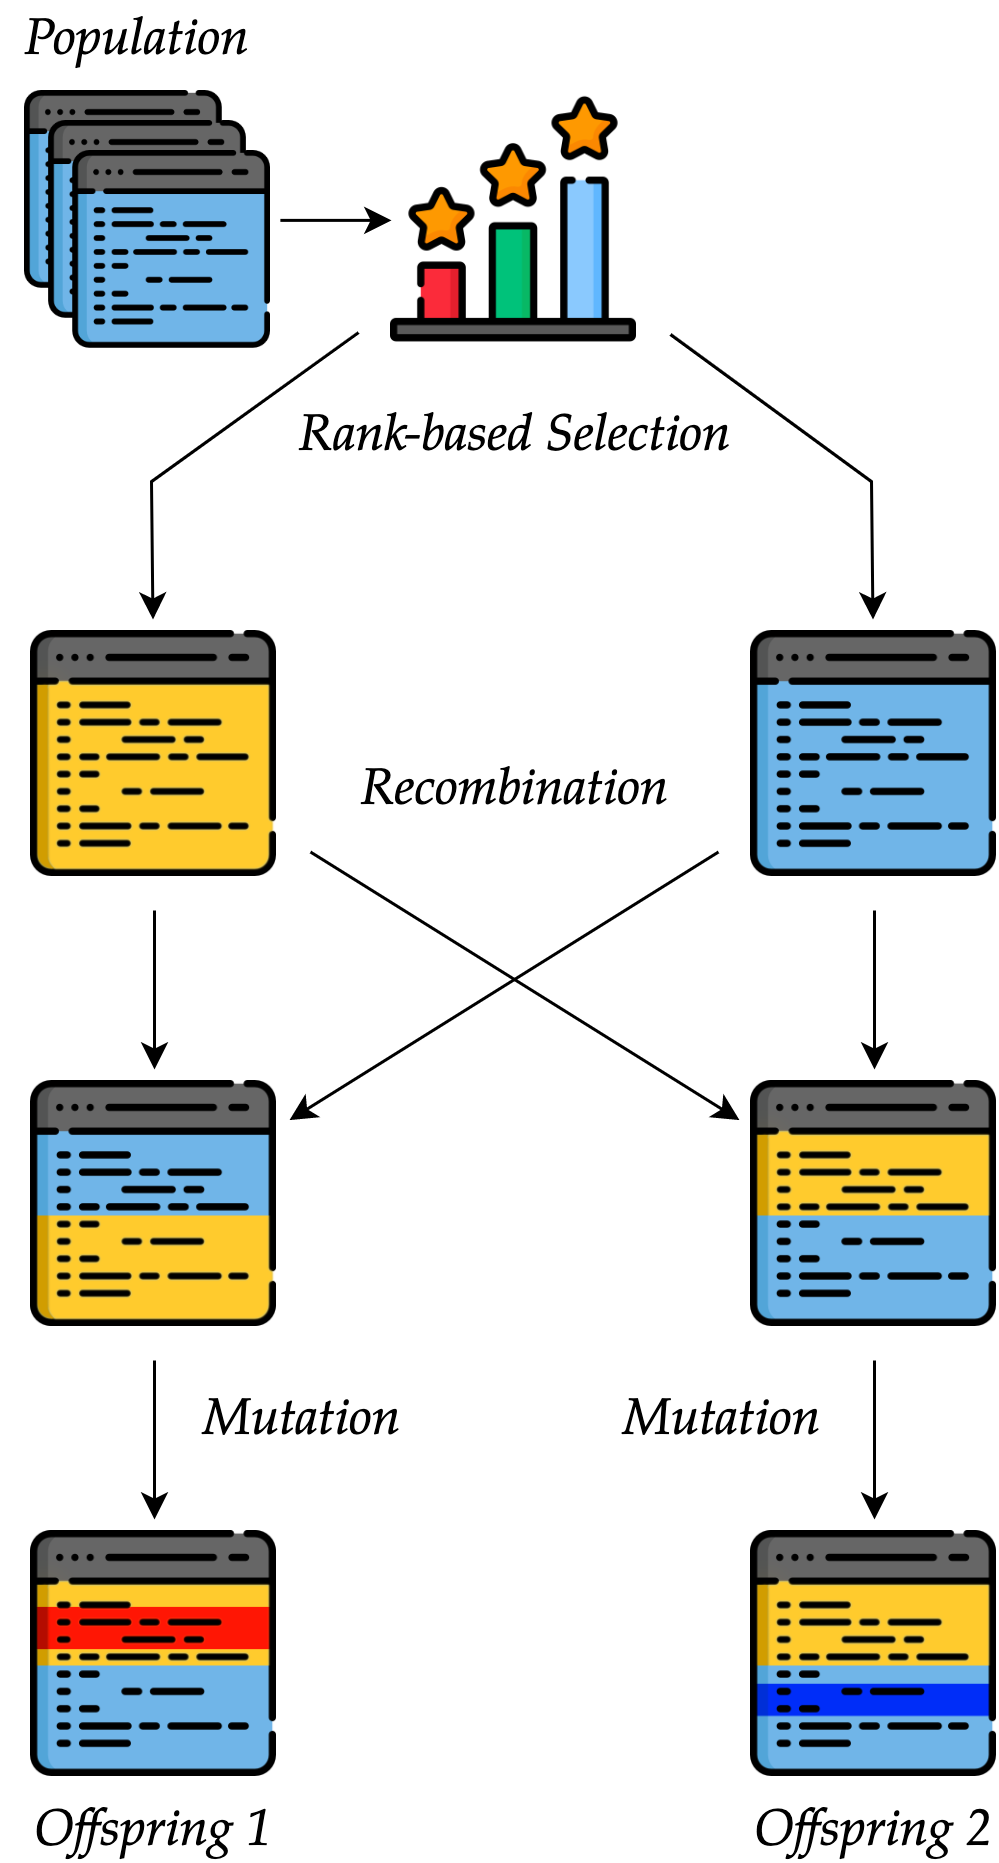
\includegraphics[width=0.5\textwidth]{ga/ga-overview}
\end{figure}

After selection and crossover have been applied, the offspring can mutate. There are different ways of mutating a sequence-based test case, e.g., delete, insert, or modify a statement~\cite{Fraser2012}. Modifying a statement includes changing the parameters of a function or replacing the function invocation itself with another one. The rules defined in \Cref{sec:problem-representation} determine when the offspring is valid with respect to the Rust compiler, e.g., replacing the function call\texttt{fn foo(\string&self)} by \texttt{fn bar(self)} is not allowed if the callee of the function is also used by another statement in some way later in the sequence because the \texttt{bar} moves the its argument.

\subsection{Crossover}
\tech applies the simplest type of crossover, the single-point crossover, which cuts two test cases at a random position and generates two new ones by swapping the subsequences of their statements~\cite{Fraser2012}. Sice the tool models chromosomes in the natural way, i.e., as a sequence of statements, when recombining a pair of chromosomes, attention must be paid to the data dependencies between individual statements. For instance, there is a dependency between a function call and its arguments, which we always declare and initialize in separate statements; that is, we use the \ac{SSA} form for the generated tests. If the intersection of a recombination hits such a dependency between statements, the offspring will not be accepted by the compiler in most cases and needs postprocessing. Tonella~\cite{Tonella2004} has proposed two solutions to this problem:

\begin{itemize}
    \item Missing dependencies of statements can be added by generating, as with the mutation operator. If certain definitions become redundant because their later use has been pushed into another choromosome by recombination, they can be deleted.
    \item Dependencies from a part of a chromosome shifted by recombination are also shifted to another chromosome regardless of the crossover point, provided they are no longer needed in the original chromosome, otherwise they could be copied.
\end{itemize}

For recombination, \tech exploits the first option: in case a recombined test case misses some data dependencies, the tool regenerates them afterwards using the \texttt{GenObject} algorithm, so that the test case becomes compilable again. \Cref{fig:crossover-example} illustrates an example for such scenario. A random intersection in the two test cases blue and green is determined. By recombining the statements, two new test cases are created, both of which, however, cannot be compiled as is since both the left (\texttt{hashmap\string_0}) and the right test case (\texttt{f64\string_0}) utilize objects that are not defined in the respective tests after all. To recover, \tech rerforms a postprocessing step to repair the broken tests (marked red).

\begin{figure}[h]
\caption{Crossover between two test cases with postprocessing}
\centering
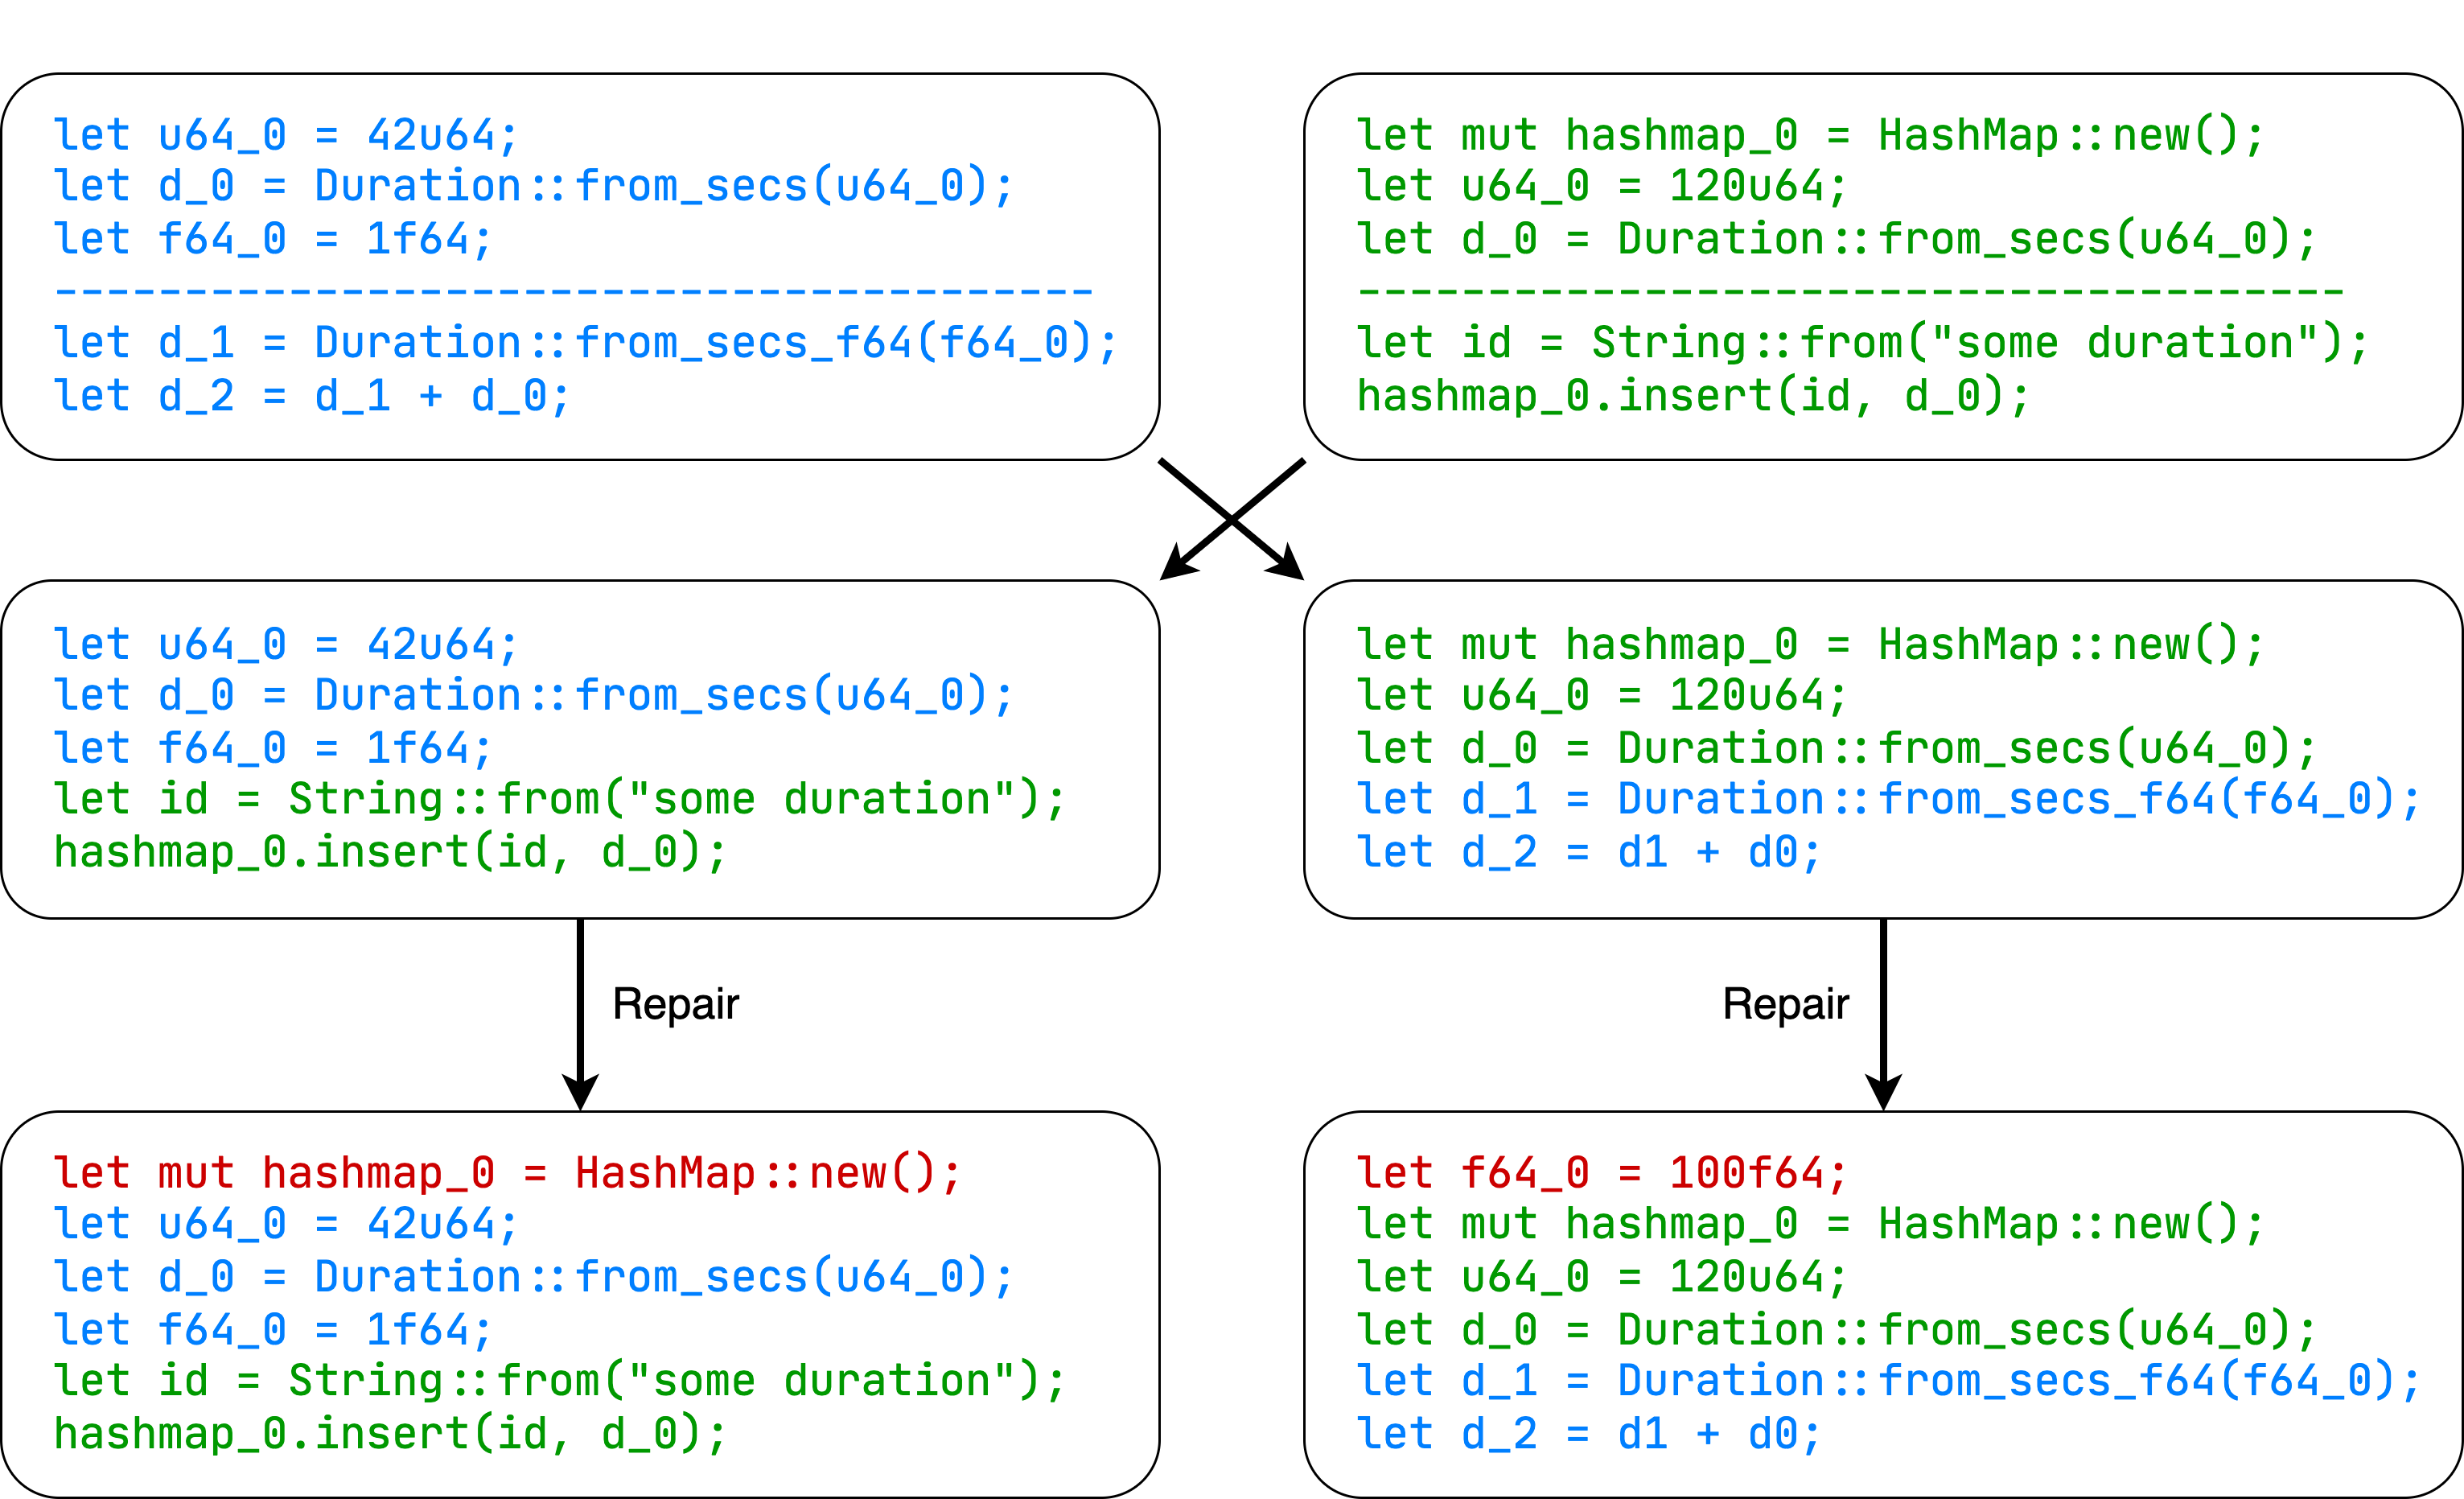
\includegraphics[width=\textwidth]{crossover}
\label{fig:crossover-example}
\end{figure}

The way \tech applies recombination can make some variables redundant, such as the \texttt{hashmap\string_0} instance in the right recombined test case. Such statements add no value to a test case and make it unnecessary longer and less comprehensible. We cannot not know in general which statements are useful, i.e., increase coverage, and which are not, unless we remove them one by one from a test case and re-run it. However, we apply a simple heuristic: we remove statements whose value is not used by any other statement in a test case in case a statement is primitive or the item it invokes is declared outside of the \sut.

\subsection{Mutation}
\tech models a test case as sequence of statements. Accordingly, we need to specify possible atomic operations for a mutation. To this end, we adopt Fraser's and Arcuri's~\cite{Fraser2012} definition of the mutation for Rust. Accordingly, \tech can performs the following operations when mutating a test:
\begin{description}
  \item[Insert a statement] A given test case $t$ is extended with a probability $\sigma$ by a new statement, which is inserted at a random position~$i$ in $t$. A new statement can only be inserted if $l(t) < L$, i.e., if the test length does not exceed a defined maximum. For each insertion, with probability $1/3$ a random call out of the pool of callables is inserted, with probability $1/3$ a method call on a value in the set $\{v(s_k) \left|~0 \leq k < i \right\}$ is used as a parameter in a random call. Any parameters of the selected invocation are either reused out of the set $\{v(s_k) \left|~0 \leq k < i \right\}$ or randomly generated. Each parameter~$p$ selected from $\{v(s_k) \left|~0 \leq k < i \right\}$ must be usable by the invocation according to the rules in \Cref{sec:problem-representation}. Multiple statements can also be inserted repeatedly; this can happen with probability~$p(n) = 0.5^n$ with~$n$ being the number of calls inserted so far. That is, after each insertion, a random decision is made whether to repeat the mutation~\cite{Tonella2004}.

  An example in \Cref{lst:mutation-invocation-insertion} demonstrates how two additional function calls \texttt{push} and \texttt{len} on an existing vector instance have been inserted in Lines~\ref{line:insert-mutation:push-on-vec} and~\ref{line:insert-mutation:len-of-vec}, respectively. Since \texttt{push} requires one argument, a 32-bit integer in this case, it has also been generated.

  \begin{lstlisting}[style=boxed, label=lst:mutation-invocation-insertion, caption={The functions \texttt{push} and \texttt{len} have been selected randomly to be invoked on \emph{vec\string_0}. An appropriate argument has been generated for the second \emph{push}, too}, escapechar=§]
  #[test]
  fn test() {
    let usize_0 = 32;
    let mut vec_0 = Vec::with_capacity(usize_0);
    let i32_0 = 45;
    vec_0.push(i32_0);
  }

  // became

  #[test]
  fn test() {
    let usize_0 = 32;
    let mut vec_0 = Vec::with_capacity(usize_0);
    let i32_0 = 45;
    vec_0.push(i32_0);
    let i32_1 = 106;
    vec_0.push(i32_1); §\label{line:insert-mutation:push-on-vec}§
    let usize_1 = vec_0.len(); §\label{line:insert-mutation:len-of-vec}§
  }
  \end{lstlisting}

  \item[Change a statement] For a test case $t = (s_1, s_2, \dots, s_l)$ with length~$l$, each statement~$s_i$ is changed with probability $1/n$. If $s_i$ is a primitive statement, then the numeric value represented by $s_i$ is changed by a random value in $\pm[0,\Delta]$ where $\Delta$ is a constant. If $s_i$ is not a primitive statement, then either a method, function, or a field with the same return type as $v(s_i)$ and parameters satisfiable with the values in the set $\{v(s_k) \left|~0 \leq k < i \right\}$ is randomly chosen or the arguments $a_1, \dots, a_n$ of $s_i$ are changed with the probability $1/n$. Each changed argument $a_x$ is replaced by a random value out of the set $\{v(s_k) \left|~0 \leq k < l \right\}$ or a generated value. The new value must again satisfy the rules defined in~\Cref{sec:problem-representation}. In \Cref{lst:mutation-input-value}, the first argument (vector instance) of the method call \texttt{push} was replaced by another one, which was generated on-the-fly because no other instance of the same type existed in the test before.

  \begin{lstlisting}[style=boxed, label=lst:mutation-input-value, caption={The first argument (which effectively is the method owner) of the call to \emph{push} in~Line~\ref{line:change-mutation:change-push-method} has been changed to a newly created value \emph{vec\string_1}}, escapechar=§]
  #[test]
  fn test() {
    let usize_0 = 32;
    mut vec_0 = Vec::with_capacity(usize_0);
    let i32_0 = 45;
    vec_0.push(i32_0);
    let i32_1 = 106;
    vec_0.push(i32_1);  §\label{line:change-mutation:change-push-method}§
    let usize_1 = vec_0.len();
  }

  // became

  #[test]
  fn test() {
    let usize_0 = 32;
    let mut vec_0 = Vec::with_capacity(usize_0);
    let i32_0 = 45;
    vec_0.push(i32_0);
    let i32_1 = 106;
    let mut vec_1 = Vec::new();
    vec_1.push(i32_1);
    let usize_1 = vec_0.len();
  }
  \end{lstlisting}

  \item[Delete a statement] For a test case $t = (s_1, s_2, \dots, s_l)$ with length~$l$, each statement~$s_i$ can be deleted with probability~$1/l$. As the value $v(s_i)$ might be used as an argument in any of the statements $s_{i+1}, \dots, s_l$, the test needs to be repaired to remain valid. For each statement $s_j$, $i < j \leq l$, if $s_j$ refers to $v(s_i)$, then this argument is replaced with another value out of the set $\{v(s_k) \left|~0 \leq k < j \wedge k \neq i \right\}$ which has the same type as $v(s_i)$ and is allowed to be used according to the rules from \Cref{sec:problem-representation}. If this is not possible, then $s_j$ is deleted as well recursively~\cite{Fraser2012}. In \Cref{lst:mutation-invocation-removal}, an instance of a vector was deleted, affecting the method calls on that instance as well. For the \texttt{push} method call, there is no alternative instance of the same type. Since it does not return any value, it can simply be eliminated because no other statements make use of it. The call to the \texttt{len} method was transferred to the other instance of the same type present in the test (\texttt{vec\string_1}). If there were no second instance of the same type in the test, or it was already consumed at this point, the statement would be have been removed, too.

  \begin{lstlisting}[style=boxed, caption=, label=lst:mutation-invocation-removal, caption={The definition of \emph{vec\string_0} in~Line~\ref{line:delete-mutation:remove-vec0} has been deleted, and statements that used it have been updated}, escapechar=§]
  #[test]
  fn test() {
    let usize_0 = 32;
    let mut vec_0 = Vec::with_capacity(usize_0);
    let i32_0 = 45;
    vec_0.push(i32_0); §\label{line:delete-mutation:remove-vec0}§
    let i32_1 = 106;
    let mut vec_1 = Vec::new();
    vec_1.push(i32_1);
    let usize_1 = vec_0.len();
  }

  // became

  #[test]
  fn test() {
    let usize_0 = 32;
    let i32_0 = 45;
    let i32_1 = 106;
    let mut vec_1 = Vec::new();
    vec_1.push(i32_1);
    let usize_1 = vec_1.len();
  }
  \end{lstlisting}
  %The call to \texttt{a.f(b)} was randomly selected for deletion. Since it was the only place where \texttt{b} was used, it was also deleted. Similar to inserting method calls, this operator can be applied repeatedly with probability~$p(n) = 0.5^n$, where $n$ is the number of deleted statements.

\end{description}


% TODO section about selection!!

\section{Dependencies}
\label{sec:dependencies}
Assume a Rust program as shown in~\Cref{lst:example-rust-program}, which consists of a struct type for rectangles and a struct that performs operations on the rectangle.
\begin{lstlisting}[style=boxed, caption={Rectangle data type}, label=lst:example-rust-program]
struct Rectangle {
    width: u64,
    height: u64,
}

impl Rectangle {
    pub fn new(width: u64, height: u64) -> Self {
        Rectangle { width, height }
    }
    pub fn width(&self) -> u64 {
        self.width
    }
}

struct Calculator {}

impl Calculator {
    pub fn new() -> Self {
        Calculator {}
    }
    pub fn area_by_value(&self, r: Rectangle) -> f64 {
        r.height as f64 * r.width as f64
    }
}
\end{lstlisting}

An example test case for the program can look like in \Cref{lst:example-testcase}. Here, a rectangle of a given length and width is created and consumed by the \texttt{Calculator} to determine the area of the rectangle. Rust's type system does not allow the variable~\texttt{calculator\string_0} to be used again. If used twice, the compiler would produce an error indicating the incorrect usage of the variable. Thus, after the statement in~Line~\ref{line:variable-moved}, the attributes of the rectangle cannot be accessed, nor can the instance serve as an argument for further calls.

\begin{lstlisting}[style=boxed, escapechar=§, caption={An example test case generated for the program in \Cref{lst:example-rust-program}}, label=lst:example-testcase]
#[test]
fn test_area_by_value() {
  let mut rectangle_0 = Rectangle::new(205u8, 166u8);
  let u64_0 = rectangle_3.width();
  let mut calculator_0 = Calculator::new();
  let f64_4 = calculator_0.area_by_value(rectangle_0); §\label{line:variable-moved}§
}
\end{lstlisting}

\section{Fitness Function}
\label{sec:fitness-function}
% Um die Selektion von Parents für die nachkommende Generationen besser guiden zu können, werden alle Individuen in einer Population nach ihrer Fitness ausgewertet. Eine gute Fitnessfunktion ist sehr wichtig bei der Suche nach Lösungen. Lösungen, die in einer bestimmten Weise ''besser'' als andere sind, sollen mit besseren Fitnesswerten belohnt werden. Was auch immer eine bessere Fitness ist, eine höhere oder niedrigere Fitness hängt davon ab, ob die Suchstrategie versucht, die Fitnessfunktion zu maximieren oder zu minimieren~\cite{McMinn_2004}.

In order to better guide the selection of parents for future generations, all individuals in a population are evaluated according to their fitness. A good fitness function is very important in the search for solutions. Solutions that are better than others in a certain way should be rewarded with better fitness values. Whatever is a better fitness, a higher or lower fitness depends on whether the search strategy tries to maximize or minimize the fitness function~\cite{McMinn_2004}.

In the search, we use branch coverage, i.e., each branch is a target. When a branch is executed, the corresponding test is marked as good with respect to this target. If a function or method is executed but a branch is not, then the fitness determines the distance of the respective test case to an execution of the target. We use the widely used definition of fitness for branch coverage, \emph{approach level} and \emph{branch distance} computation, which is used in search-based generation of test data~\cite{McMinn_2004}. The approach level describes how far a test case was from a target in the \cdg when the test case deviated from the course. We compute approach level in terms of the number of missed control dependencies between the target and the point where the test case took a wrong turn. Approach level is equal to $0$ if all control dependency edges were reached by the test case.

% TODO reword
The branch distance estimates how far the branch at which execution diverged is from evaluating to the necessary outcome. To determine these values, the test case has to be executed once on the unmodified software. If the target executed, then approach level and branch distance are $0$. Otherwise, the rules from \Cref{tab:local-branch-distance-formulas} are used for calculation of numeric values. For all other cases, the local branch distance is either $0$ or $1$ depending on whether the respective branch was executed or not. Assume the function \texttt{bar} from \Cref{lst:example-branch-distance-boolean-flag} which takes a boolean named \texttt{flag}. When called \texttt{bar(true)}, the branch distance for the \emph{true} branch is $0$ since it gets executed, while the branch distance for the \emph{false} branch is $1$ because we do not know how the boolean value has been computed. It could be a result of some numbers comparison, a function call, or just a constant. Figuring that out requires inter-procedural static analysis and advanced \mir instrumentation that \tech currently does not apply.

\begin{lstlisting}[style=boxed, caption={Computation of local branch distance for a boolean flag that we do not know where it came from}, label=lst:example-branch-distance-boolean-flag]
fn bar(flag: bool) {
    if flag {
      println!("Flag is true");
    } else {
      // ...
    }
}
\end{lstlisting}

Of course, not every program uses only comparisons of numbers and thus many values for the branch distance will be binary. This means that the approach level has a much more important meaning for the search. Consider the following example function \texttt{foo}:

\begin{lstlisting}[style=boxed, caption=, label=lst:example-branch-distance-nesting, escapechar=§]
fn foo(x: i32, y: i32) -> i32 {
    if x < 5 {
        if y >= 10 { §\label{line:fitness-example:outer-true-start}§
            0 §\label{line:fitness-example:inner-true}§
        } else {
            1 §\label{line:fitness-example:inner-false}§
        } §\label{line:fitness-example:outer-true-end}§
    } else {
        2 §\label{line:fitness-example:outer-false}§
    }
}
\end{lstlisting}

Assume that a test invokes \texttt{foo}. In \Cref{tab:example-fitness-calculation}, calls to \texttt{foo} with various arguments and the resulting approach level (AL) and branch distance (BD) are shown as examples .
\begin{table}[h!]
\centering
\begin{tabular}{c|cc|cc|cc}
\hline
& \multicolumn{2}{c|}{\textbf{foo(0, 5)}}                     & \multicolumn{2}{c|}{\textbf{foo(6, 1)}}                      & \multicolumn{2}{c}{\textbf{foo(0, 10)}}                     \\
\cline{2-7}
\textbf{Branch (Line)} & AL & BD & AL & BD & AL & BD \\
\hline
\ref{line:fitness-example:outer-true-start}-\ref{line:fitness-example:outer-true-end} & 0                       & 0                        & 0                       & 2                        & 0                       & 0                        \\
\ref{line:fitness-example:outer-false}                      & 0                       & 5                        & 0                       & 0                        & 0                       & 5                        \\
\ref{line:fitness-example:inner-true}                      & 0                       & 5                        & 1                       & 2                        & 0                       & 0                        \\
\ref{line:fitness-example:inner-false}                      & 0                       & 0                        & 1                       & 2                        & 0                       & 1 \\ \hline
\end{tabular}
\caption{Fitness value calculation for different invocations of \texttt{foo}}
\label{tab:example-fitness-calculation}
\end{table}

% TODO reword
As usual in the \ac{SBST} literature, the branch distance should not dominate the approach level; thus, the former is normalized in the range $[0, 1]$, for instance, using the following normalization function proposed by Arcuri~\cite{Arcuri_2011}:

\[\alpha(x) = \frac{x}{x + 1}\]

This allows us to calculate the overall fitness of a test~$t$ with respect to target~$m$:
\[D_m(t) = \text{Approach Level} + \alpha(\text{Branch Distance})\]

\begin{table}[]
\centering
\begin{tabular}{lcr}
\hline
\textbf{Condition}  & \textbf{Distance True} & \textbf{Distance False} \\
\hline
x == y              & |x - y|                & 1                       \\
x != y              & 1                      & |x - y|                 \\
x \textgreater y    & y - x + 1              & x - y                   \\
x \textgreater{}= y & y - x                  & x - y + 1               \\
x \textless y       & x - y + 1              & y - x                   \\
x \textless{}= y    & x - y                  & y - x + 1               \\ \hline
\end{tabular}
\caption{Local branch distance calculation for numeric values}
\label{tab:local-branch-distance-formulas}
\end{table}

\section{Test Oracles and Testability Transformations}
\label{sec:testability-transformations}

A technique called \emph{testability transformation} tries to overcome this obstacle. A testability transformation is a source-to-source program transformation that seeks to improve the performance of some chosen test data generation technique~\cite{Harman2004}, e.g., reach difficult branches. Beyond that, a \sut can be transformed in a way such that artificial branches are inserted into the code to guide the search into triggering some exceptional behavior and crash the program. For instance, \textsc{EvoSuite}~\cite{Fraser2013} employs multiple testability transformations such as array access transformation (\Cref{lst:evosuite-array-access-transformation}), division by zero transformation, or numerical overflow transformation. Those transformations do not increase code coverage in general but contribute to discovering potential unforeseen behavior and generating inputs that trigger it.

\begin{lstlisting}[language=Java, style=boxed, caption={Array access transformation in \textsc{EvoSuite} for Java}, label=lst:evosuite-array-access-transformation]
// Original method
void foo(int x) {
  bar[x] = 0;
}

// Transformed method for better testability
void foo(int x) {
  if (x < 0) {
    throw new NegativeArraySizeException();
  }
  if (x >= bar.length) {
    throw new ArrayIndexOutOfBoundsException();
  }
  bar[x] = 0;
}
\end{lstlisting}

With the new branches in place, artificial coverage objectives are created that a \ga can often compute meaningful distances for, which significantly improves the effectiveness of a \ga in this regard compared to random search. We apply similar ideas to \tech. However, some of the problems that other programming languages have, do not affect (safe) Rust, e.g., there are no null pointers as in C or Java, for which we can weave explicit if conditionals to check nullity. Moreover, the Rust compiler already incorporates checks for common issues in the \mir that are addressed by testability transformations. That is, we do not have to transform the \mir to introduce new branches as in~\Cref{lst:evosuite-array-access-transformation}, but only trace these branches automatically inserted by the compiler.

\section{Seeding Strategies}
\label{sec:seeding-strategies}
According to Fraser's and Arcuri's definition~\cite{6200103}, seeding refers to techniques that make use of previous related knowledge to help solve the testing problem given.

A \ga usually starts with a random population with constants being chosen randomly, too, in the initial population or during the search. However, domain knowledge of the testing problem given can be exploited to construct the population. \tech applies multiple seeding strategies that are described in the following to improve the effectiveness and performance of the search.

\begin{description}
  \item[Seeding Constants] Execution flow of complex nested code often depends on specific values, i.e., branch conditions containing constants or string comparisons that perform a constant substring verification. Some search-based tools make use of such data by collecting them from the source code and then seeding the search with the values. \tech also implements this technique and extracts constant values from the \mir of a \sut. Even though utilizing the extracted constants does not necessarily result in covering a branch (e.g., we will not cover the true branch of \texttt{if x < 2} with \texttt{x = 2}), those values are often very close to the required ones and can be improved by mutation. With the extracted constants in-place, \tech employs them with a certain probability~$p_{mir}$ whenever a constant must be generated during the search, for instance, to satisfy a parameter of a function invocation.
  \item[Seeding Functions] The strategy to generate new test case individuals as described in~\Cref{alg:gentest} does not guarantee that all of the functions out of the pool~$M$ will be incorporated in the generated tests and thus, executed, which is a prerequisite for higher code coverage and better fitness. Therefore, \tech provides the ability to sort the pool of possible functions into a ring buffer and pick them one-by-one from the buffer each time a new function invocation shall be generated during the initialization of the initial population. In this way, \tech achieves that all practically possible functions are at least entered once in the final test suite. This is ensured by the fact that an function entry is an objective itself, too, so the test that covers it remains in the archive.
\end{description}


\clearpage
\chapter{Implementation}
\label{chap:implementation}
In this chapter we present essential parts of the implementation of \tech. To generate tests for a crate, \tech has to complete several intermediate steps that \Cref{fig:rustyunit-overview} illustrates. First and foremost, the tool requires the information about which data types the \emph{Crate} has and which functions the data types provide in order to be able to model meaningful tests in the first place. Therefore, it performs a \hir analysis, which yields a collection of \emph{Generators}. \todo{Generators inkludiert irgendwie eher nur Funktionen und weniger Datentypen an sich}. These provide an overview of which data types can be instantiated in a test case, and which methods can be invoked on those instances. \tech also derives the ownership rules at this point, e.g., whether and how multiple statements may use a certain variable in a valid way, as described in~\Cref{sec:problem-representation}.

To evaluate the \emph{Generated Tests} in terms of their coverage, \tech instruments the \mir and compiles the crate yielding an \emph{Instrumented Binary}. During instrumentation, the tool injects instructions into the \mir to trace the execution of individual basic blocks and branches. If a generated test executes a code location in the crate, the event (and the corresponding branch distance to another branch in case it has been a branch) is stored in the \emph{Execution Traces}.

The execution traces only contain a raw part of the fitness values. To calculate the overall fitness value with respect to each coverage target, \tech must additionally determine the approach level from the corresponding \emph{Control Dependence Graphs}, as described in~\Cref{sec:fitness-function}. It computes the graphs of execution units contained in the crate by analyzing its \mir. This implies building a post-dominator tree from the \cfg, which a \mir effectively is, and then computing the control dependencies. With the \cdgs and execution traces in place, \tech computes how good a certain test with respect to the coverage targets, select the fittest ones and stores them into the \emph{Archive}. Now \tech can either generate a new population and evolve it in the next iteration, as already shown in~\Cref{fig:ga-overview}, or, when the search budget is exhausted, return the archive, i.e., the best test cases found up to that point in the form of Rust source code.

In the next sections we explain how \tech performs the outlined steps by hooking into the compiler in detail.

% Die Übesicht des ganzen Prozesses
\begin{figure}[h!]
\caption{The architecture of \tech}
\centering
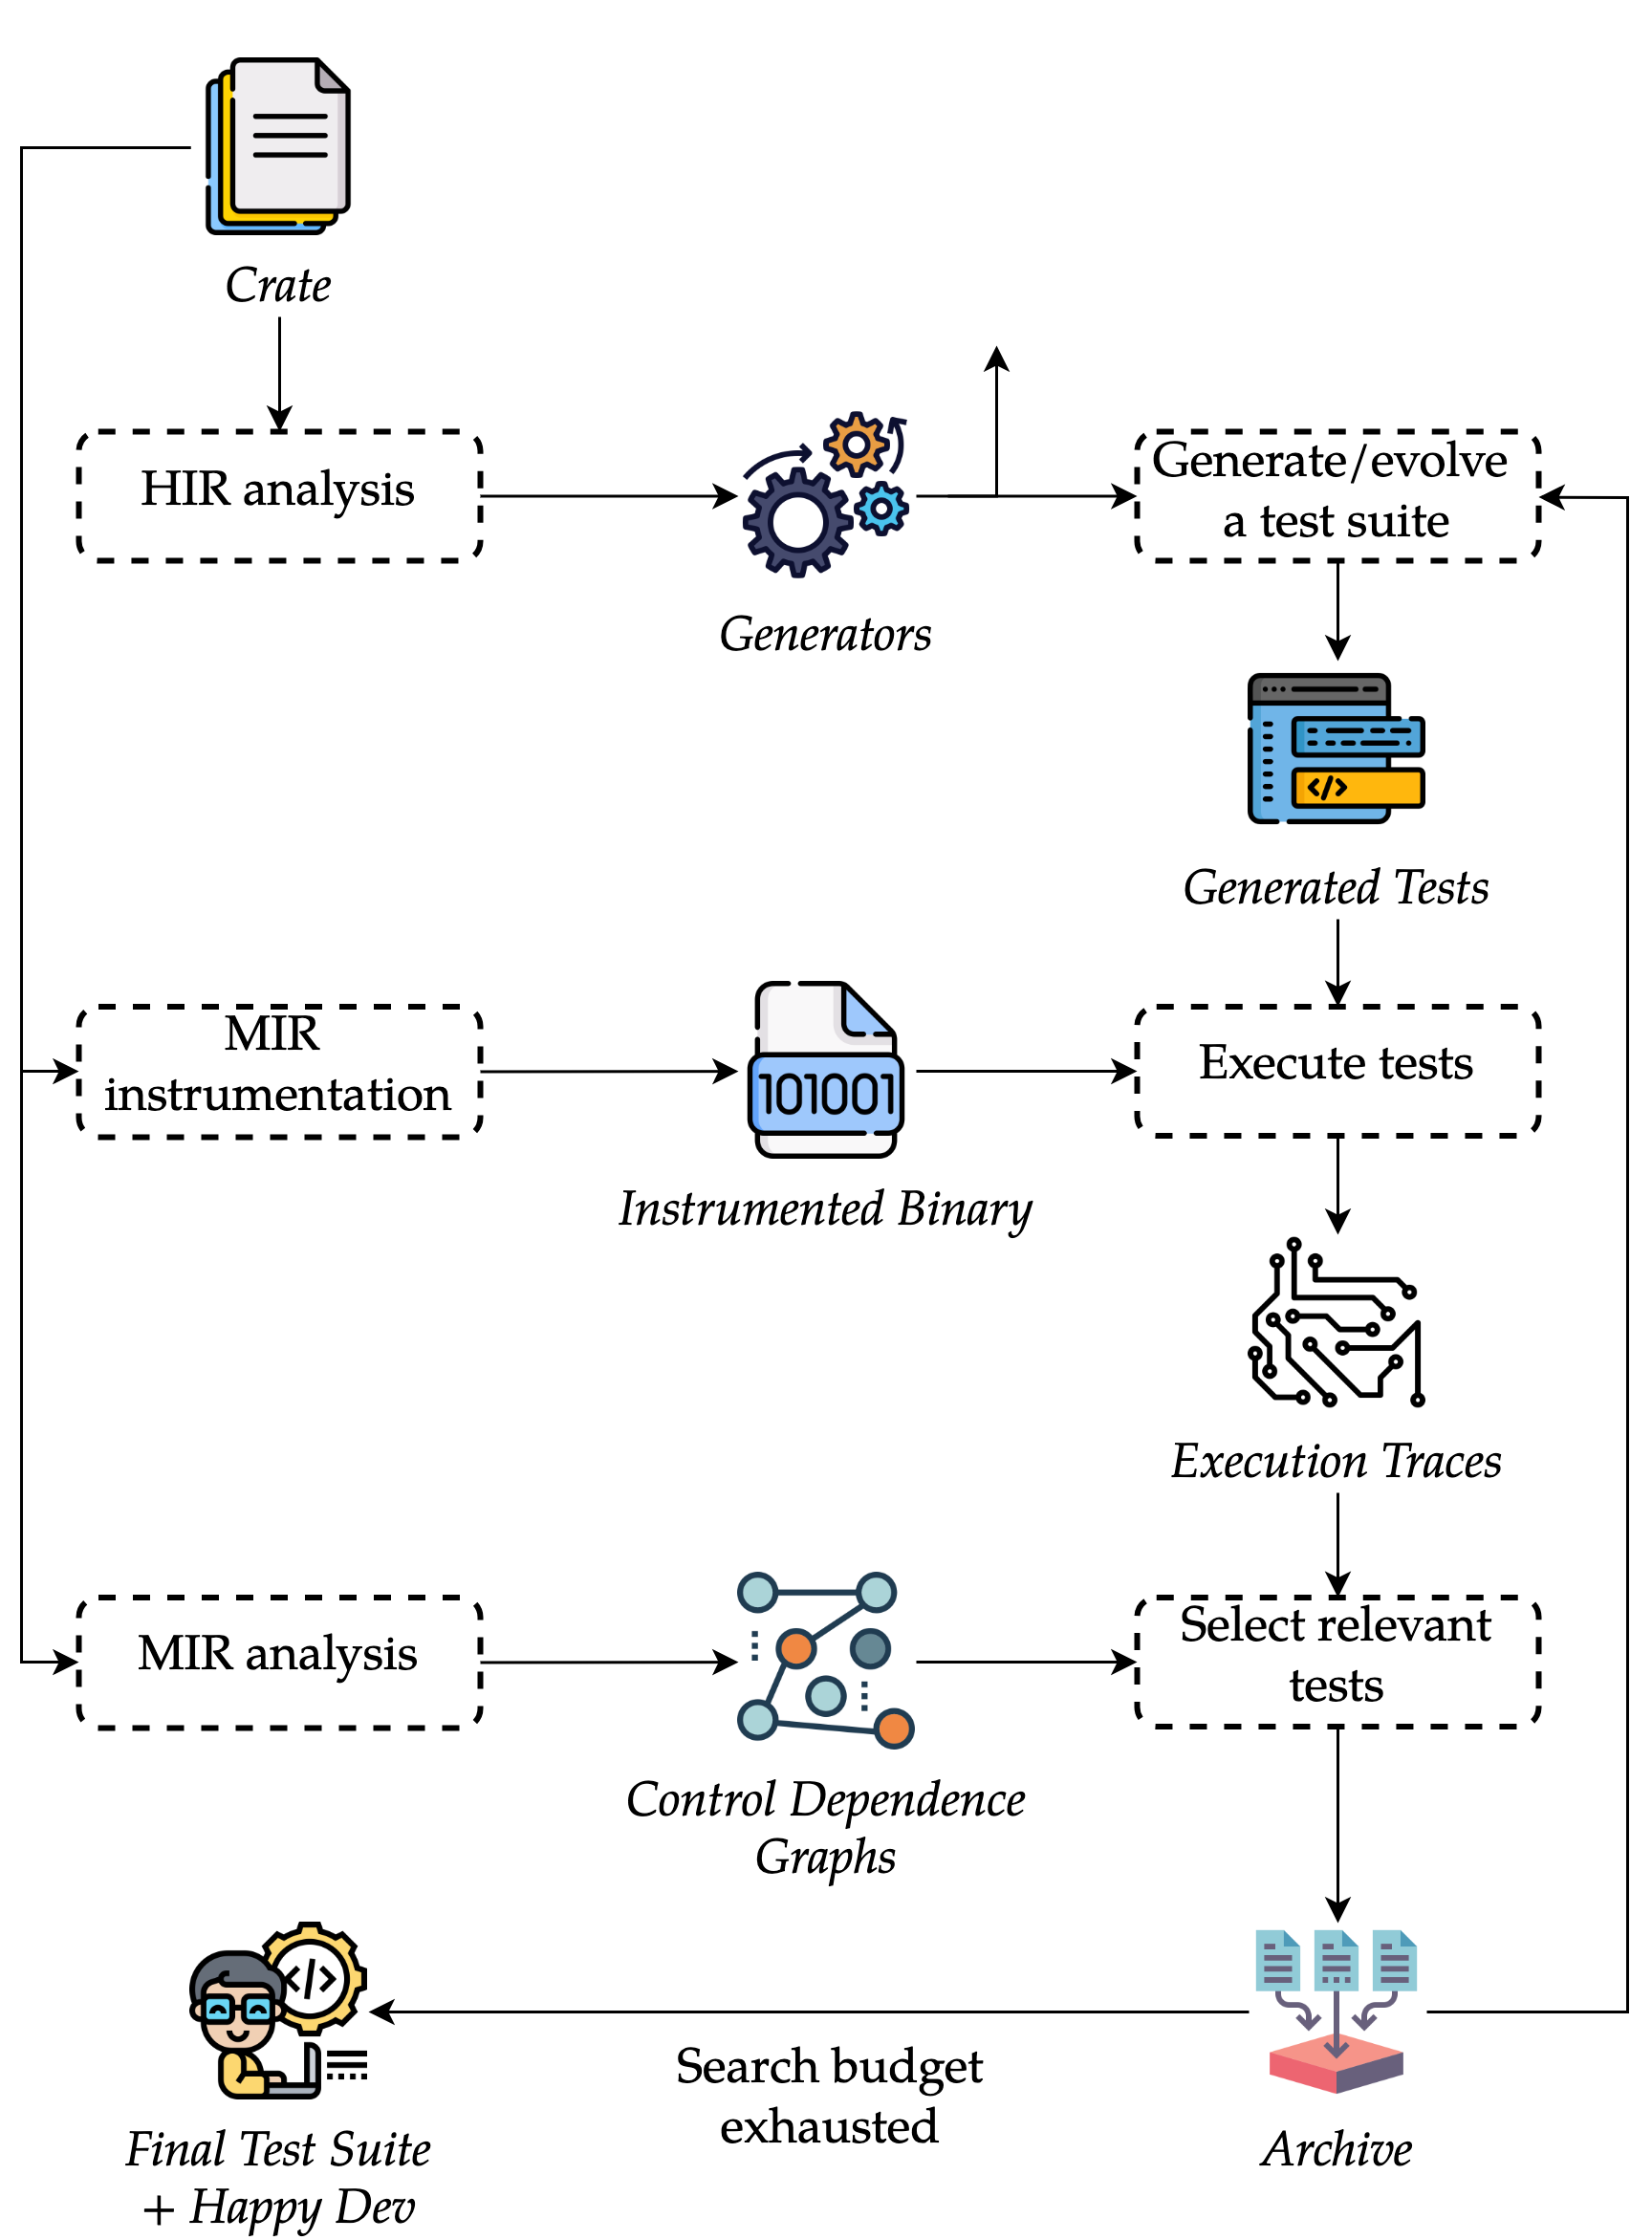
\includegraphics[width=\textwidth]{overview/overview-enhanced}
\label{fig:rustyunit-overview}
\end{figure}

\section{Using the Compiler Hooks}
The Rust compiler design makes it possible to use it both, as an executable and as a collection of libraries. To this end, Rust provides compiler crates, which can be recognized by their common prefix, \texttt{rustc}, such as \texttt{rustc\string_driver}, which is an interface for running the compiler programmatically.

To have access to the compiler internals, multiple things are required. Firstly, the internals are not stable and probably will never be. As such, programs that use compiler internals must use \emph{nightly} versions of the toolchain. Secondly, the crates must have the \texttt{rustc\string_private} feature enabled, which allows crates to access individual compiler crates. Thirdly, these crates must be explicitly specified in the crate root using the \texttt{extern crate} keywords. For instance, if the program needs the internal \texttt{rustc\string_driver}, it must specify it the following way in the crate root: \texttt{extern crate rustc\string_driver}.

With compiler internals available, we can implement some of the callbacks that the compiler will call at appropriate point of time. The \texttt{rustc\string_driver::Callbacks} trait defines four callbacks, which are called in the following order:
\begin{enumerate}
    \item \texttt{config}
    \item \texttt{after\string_parsing}
    \item \texttt{after\string_expansion}
    \item \texttt{after\string_analysis}
\end{enumerate}

The \texttt{config} method will be called before creating the compiler instance and allows to change the default compiler configuration. Each of the other three functions will be called after the end of the corresponding compilation phase. The interface provides the \texttt{after\string_*} hooks with an instance of the compiler and, more important, with a \texttt{Queries} object which allows to query the global context of the crate under compilation. It is very convenient because this way we can extract all the items defined in a crate, including functions and methods along with their parameters and return types. %We need this data to know what statements can be placed in a generated test.

The sequence of the callbacks is called for each crate and its dependencies since each crate is compiled separately, with the \sut coming last after its dependencies have been processed. This theoretically also provides us the ability to analyze the code structure of the dependencies in case some of the \sut's functions required a parameter of an external type. However, this does not work for the standard library of the language as it usually already comes precompiled. Thus, \tech is not able to extract this data automatically and therefore, would not know how to initialize and manipulate a vector (\texttt{std::vec::Vec}), for example. However, since the data is essential for generating tests for most of the crates, \tech includes prepared types from the standard library and their functions relevant to the case study subjects.

\begin{lstlisting}[style=boxed, caption={We can register a listener function to analyze the code structure of the compiled crate}, escapechar=§, label=lst:optimized-mir]
fn after_analysis(&mut self, _c: &Compiler,
    _q: &'tcx Queries<'tcx>) {
  _q.global_ctxt().map(|ctxt| ctxt.peek().enter(analyze)) §\label{line:enter-tyctxt}§
}

fn analyze(tcx: &TyCtxt<'_>) {
  // Obtain the MIR instance of a function
  let mir = tcx.optimized_mir( §\label{line:optimized-mir-call}§
    // Some id
  );

  // Extract types and CDGs
}
\end{lstlisting}

Within the callbacks, with a compiler and a \texttt{Queries} object given, we can access the \acp{IR} of the crate under compilation, e.g., we can query the \mir of a function body by its \texttt{DefId}, as shown in~\Cref{lst:optimized-mir}. To this end, we retrieve the \texttt{TyCtxt} instance in~Line~\ref{line:enter-tyctxt}, which is the central data structure of the compiler and provides methods to query different regions of the compiled code, e.g., \texttt{optimized\string_mir} in~Line~\ref{line:optimized-mir-call} to obtain the \mir of a function. We cannot modify it and pass the modified version back to the compiler, though, which is critical for \mir instrumentation. This is not a concern for the \hir and \mir analysis, as we only want to read the structure of the crate. For this purpose, we can override the default implementation of the \texttt{optimized\string_mir} method with a custom one. The \texttt{config} callback provides a mutable \texttt{Config} object which allows to replace many of the query functions.

\begin{lstlisting}[style=boxed, caption={The Rust compiler interface accepts an object which implements its callback trait, allowing us to execute code at different compilation phases}, label=lst:compiler-callbacks, escapechar=§]
struct CompilerCallbacks;

type mir_fn_ptr = for<'tcx>
  fn(_: TyCtxt<'tcx>, _: DefId) -> &'tcx Body<'tcx>;

impl rustc_driver::Callbacks for CompilerCallbacks {
  fn config(&mut self, _config: &mut Config) {
    _config.override_queries = Some(|_, _, external| { §\label{line:mir-provider-start}§
      let fn_ptr: mir_fn_ptr = |tcx, def_id| {
        let opt_mir §\label{line:obtain-default-mirprovider-start}§
          = rustc_interface
            ::DEFAULT_EXTERN_QUERY_PROVIDERS
            .borrow().optimized_mir; §\label{line:obtain-default-mir-provider-end}§
        // Query original MIR instance
        let mut body = opt_mir(tcx, def_id).clone(); §\label{line:query-mir}§
        let hir_id = tcx.hir()
          .local_def_id_to_hir_id(def.expect_local());

        if is_monitor(hir_id, &tcx) { §\label{line:is-monitor-check}§
          // Do not instrument our own monitor
          return tcx.arena.alloc(body);
        }

        // Instantiate MIR visitor
        let mut mir_visitor = MirVisitor { tcx };
        // Instrument the original MIR
        mir_visitor.visit_body(&mut body); §\label{line:visit-mir}§
        // Pass instrumented MIR back to compiler
        tcx.arena.alloc(body) §\label{line:return-instrumented-mir}§
      }; §\label{line:mir-provider-end}§
      external.optimized_mir = fn_ptr;
    });
  }
}
\end{lstlisting}

As shown in~\Cref{lst:compiler-callbacks}, a provider for an optimized \mir is a function pointer. Our custom provider implementation (Lines~\ref{line:mir-provider-start}-\ref{line:mir-provider-end}) is a basic wrapper, which
\begin{enumerate}
  \item first obtains the original \mir instance in~Line~\ref{line:query-mir} using the default implementation in~Lines~\ref{line:obtain-default-mirprovider-start}-\ref{line:obtain-default-mir-provider-end},
  \item verifies that the current \mir instance is not part of our own monitor in~Line~\ref{line:is-monitor-check}, otherwise skips the instrumentation,
  \item applies the \texttt{MirVisitor}, which mutates the \mir in-place, in~Line~\ref{line:visit-mir},
  \item returns the mutated version to the compiler in~Line~\ref{line:return-instrumented-mir}.
\end{enumerate}

The compiler invokes the \texttt{optimized\string_mir()} provider in further steps, and thus, propagates the mutated \mir instance.

\Cref{lst:running-compiler} shows how the Rust compiler can subsequently be started programmatically. The program accepts command line arguments intended for the compiler in~Line~\ref{line:rustc-args}, instantiates the struct implementing the aforementioned callbacks in~Line~\ref{line:instantiate-compiler-callbacks} and a compiler instance in~Line~\ref{line:init-the-compiler-start}, and runs the compiler in~Line~\ref{line:run-the-compiler}.

\begin{lstlisting}[style=boxed, caption={Running the Rust compiler like a library}, label=lst:running-compiler, escapechar=§]
fn run_rustc() -> Result<(), i32> {
  let rustc_args: Vec<String> = std::env::args() §\label{line:rustc-args}§
    .collect();

  let mut callbacks = CompilerCallbacks {}; §\label{line:instantiate-compiler-callbacks}§
  // Register the callbacks for analysis
  // and instrumentation and run the compiler
  let err = rustc_driver::RunCompiler::new( §\label{line:init-the-compiler-start}§
    &rustc_args, &mut callbacks §\label{line:init-the-compiler-end}§
  ).run(); §\label{line:run-the-compiler}§

  if err.is_err() {
    return Err(1);
  }

  Ok(())
}

fn main() {
  exit(run_rustc()
      .err()
      .unwrap_or(0)
  )
}
\end{lstlisting}

Now this program can be used in general for instrumenting Rust programs. However, calling it directly is very cumbersome, since the compiler needs to know many arguments, especially for large crates, in order to link dependencies correctly. Usually one uses a build system for this purpose, e.g., Cargo, which takes over this task and provides appropriate compiler arguments when building a crate. Fortunately, Cargo provides a way to define a custom \texttt{rustc} wrapper, which is then supplied with the arguments by Cargo. The task of such a wrapper is to eventually call the real compiler on itself and forward those argument in order to fullfil the expected behavior during compilation~\footnote{\url{http://web.archive.org/web/20220506220810/https://doc.rust-lang.org/cargo/reference/environment-variables.html}}. To use the wrapper, one has to set the environment variable \texttt{RUSTC\string_WRAPPER} to the path to the wrapper binary. Finally, a target Rust program can be built and instrumented by running:

\texttt{RUSTC\string_WRAPPER=./instrumentation cargo \string+nightly build}

Since the wrapper uses \texttt{rustc\string_private} features, we have to tell Cargo to enable the nightly channel. The next step is to define how to instrument the \mir so that we can observe the execution paths triggered by an execution of generated tests.

%The whole process starts, when we run the compiler for the first time on a target crate that we want to test. During this process we can already extract the available items like structs and their methods by traversing the \hir.

\section{HIR Analysis}
For the purpose of test generation, \hir and \mir are of primary importance. First, we are interested in all possible functions, structs/enums, and their methods and fields in the crate we want to test. This information allows us to evaluate which statements we can use in a generated test at all and what types of instances do those statements produce. We call functions and methods generators since those can generate instances and values of the required types when we recursively search for a dependency. The fact that desugaring has already been performed in the \hir has no influence at this point, because the transformations are only performed intra-procedurally. We are only interested in type and method definitions, their parameters and return types, which still remain unchanged at this level. Moreover, thanks to \hir we can also determine the absolute path of a type, for example a parameter. Relative type names, such as \texttt{File} instead of \texttt{std::fs::File}, can lead to difficulties when compiling the generated tests due to missing imports. Thus, it is easier to carry a complete type path, and by means of \hir we can easily query this.

% TODO reword
The top-level data structure in the \hir is the \texttt{Crate}, which stores the contents of the crate currently being compiled. The Rust compiler compiles crates independently and, thus, only ever constructs \hir for the current crate. Technically, the \hir \texttt{Crate} structure contains a number of maps that serve to organize the content of the crate for easier access. For instance, the contents of individual items (e.g., modules, functions, traits, impls and so on) in the \hir are not directly accessible in the parents. So, for example, if there is a module item \texttt{foo} containing a function \texttt{bar()}:

\begin{lstlisting}[style=boxed, caption={}]
mod foo() {
    fn bar() { }
}
\end{lstlisting}
then in the \hir, the representation of module \texttt{foo} would only have the ID \texttt{I} of \texttt{bar()}. To get the details of the function, we would lookup \texttt{I} in the \texttt{items} map of the \hir, as shown in \Cref{lst:hir-analysis}. One nice result from this representation is that one can iterate over all items in the crate by iterating over the key-value pairs in these maps (without the need to trawl through the whole \hir). The other reason for such decoupled design is for better integration with incremental compilation. This way, if we gain access to some item, e.g., for the module \texttt{foo}, we only gain access to the id for \texttt{bar()}, and we must invoke some functions to lookup the contents of the function given its id. This gives the compiler a chance to observe that we accessed the data for \texttt{bar()}, and then record the compilation dependency.

In \Cref{lst:hir-analysis} we iterate over the \texttt{items} map of the \hir and extract the relevant elements like functions, structs, and methods by pattern matching the type of an item. Each item stores a \texttt{Span} object, which shows its origin at the source code level, i.e., the source file it has been defined within. This is important for us because in Rust, unlike, for instance, in Java, unit tests can and should, by convention, be written into the files that contain the code to test. This also means that unit tests, also our generated tests, can invoke private functions and methods directly, which in turn can lead to better search results.

On the other hand, the ability to invoke private items leads to further constraits for our approach. We say that a test case is bound to a module, that is, a source code file, if it calls private functions from that module. When generating further statements for a module-bound test using \emph{GenTest} and \emph{GenObject} from~\Cref{alg:gentest}, \tech is only allowed to select those functions that either belong to the same module as the test at hand or are public to keep the test compilable.

% TODO also add enums and traits
\begin{lstlisting}[style=boxed, caption={Iterate over the items in the HIR of a crate}, label=lst:hir-analysis]
fn hir_analysis(
  tcx: &TyCtxt<'_>, callables: &mut Vec<Callable>
) {
  for item in tcx.hir().items() {
    match &item.kind {
      ItemKind::Fn(sig, _, _) => {
        if &item.ident.name.to_string() != "main" {
          // item is a basic function
          analyze_fn(sig, item.def_id,
            &mut callables, &tcx);
        }
      }
      ItemKind::Impl(impl_item) => {
        // item is a method
        analyze_impl(impl_item, &mut callables, &tcx);
      }
      ItemKind::Struct(s, g) => {
        // item is a struct
        analyze_struct(item.def_id, s, g, &item.vis,
          file_path.unwrap(), &mut callables, &tcx);
      }
      // ... analyze enums
      _ => {
        // Ignore other items
      }
    }
  }
}
\end{lstlisting}

With the \hir analysis set up, \tech can already generate random tests, since we know which functions can be called. \Cref{lst:hir-analysis-example} shows an example program to test. After the analysis, the following holds in terms of \Cref{alg:genobject}: $M = \{\texttt{Address::new}, \texttt{Person::new}, \texttt{Person::address}, \texttt{say\string_hello\string_to}, \texttt{address\string_to\string_string}\}$. If we wanted to execute the \texttt{address\string_to\string_string} function in an empty test $t = \{\}$, we would have to generate an argument of type \texttt{Address}. Thanks to the information about the return type of a method, we can use $GenObject(Address, \{\}, M, t)$ to create either an \texttt{Address} object using \texttt{Address::new} or \texttt{Person::address}. The latter one is a method, i.e., it expects a \texttt{self} object argument which would require us to recursively search for a way to create an object of type \texttt{Person}, e.g., by calling the constructor \texttt{Person::new}.

\begin{lstlisting}[style=boxed, caption={After HIR analysis, we know how a \texttt{Person} object can be generated to be used in \texttt{say\string_hello\string_to}.}, label=lst:hir-analysis-example]
struct Address {
  street: String,
  house_n: usize,
  city: String,
  zip: usize
}

impl Address {
  pub fn new(street: &str, house_n: usize,
  city: &str, zip: usize) -> Self {
    Address {
      street: street.to_owned(),
      house_n,
      city: city.to_owned(),
      zip
    }
  }
}

struct Person {
  name: String,
  address: Address
}

impl Person {
  pub fn new(name: &str, address: Address) -> Self {
    Person {
      name: name.to_owned(),
      address
    }
  }

  pub fn address(&self) -> &Address {
    &self.address
  }
}

fn say_hello_to(person: &Person) {
  // ...
}

fn address_to_string(address: &Address) -> String {
  // ...
}
\end{lstlisting}

\section{MIR Analysis}
In this section, we describe the analysis steps \tech performs on the \mir of a crate under test.

% Building CDG from MIR
\subsection{Control Dependence Graphs}
To improve the effectivity of generated tests, both \acp{DynaMOSA} and the fitness function (approach level) that \tech uses as described in~\Cref{sec:fitness-function}, exploit information from the \cdgs~\cite{Ferrante1987} of the \sut. A \ac{CDG} can be constructed from a \cfg and its post-dominator tree. As \mir itself is a \cfg, we can easily build the post-dominator-tree and the \ac{CDG} of each method and function we want to test. \tech does not use the complete \cfg of a \texttt{Body}, but rather a subset of it. The Rust compiler creates many unwind edges in the \mir that point to basic blocks whose task is to cleanup the heap in case the program panics at some point of its execution. However, we are not interested in the cleanup logic of the compiler. Moreover, considering unwind nodes results in \cfg having multiple exit nodes, which complicate the computation of a post-dominator tree. We filter out most of the unwind edges from a \cfg except for those described in~\Cref{sec:mir-testability-transformations}. To simplify further tree computations, we add a dummy exit node that we point all original exit nodes to, in case if there are at least two dedicated exit nodes.

The standard algorithm to compute a dominator tree from a \cfg yields a post-dominator tree when applied to reversed \cfg, given that the original \cfg has a single exit point, i.e., a single entry point with reversed edges.

Prosser~\cite{Prosser1959} introduced the notion of dominance in a 1959 paper on the analysis of flow diagrams, defining it as follows:
Box~\emph{i} dominates box~\emph{j} if every path (leading from input to output through the diagram) which passes through box\emph{j} must also pass through box~\emph{i}. Thus box~\emph{i} dominates box~\emph{j} if box~\emph{j} is subordinate to box~\emph{i} in the program. He did not specify the algorithm to compute dominance, though. Since then, several algorithms for calculating dominance have been presented. Post-dominance can be computed the same way on a \cfg with reversed edges, given that the \cfg has a single exit point. \tech exploits the \texttt{petgraph} graph library for Rust, which provides an implementation of the simple fast dominance algorithm~\cite{Cooper2001} by Cooper et al. Finally, we compute a \ac{CDG} for each method body based on the algorithm described by Ferrante et al~\cite{Ferrante1987}. At the end of this step, \tech yields a set of \cdgs, one for each function in the \sut.

% Extracting constants from the MIR
\subsection{Constant Pool Analysis}
As part of the seeding strategy for enhanced search described in~\Cref{sec:seeding-strategies}, \tech additionally performs an analysis of the constants used in the \sut to simplify the coverage of complex branches. Assume an example program that parses raw date components to a \texttt{Date} instance:
\begin{lstlisting}[style=boxed, caption={},label=lst:mir-constant-analysis-example, escapechar=§]
struct Date;

impl Date {
  fn from(day: u8, month: &str, year: u16)
      -> Result<Date, Error> {
    if month.to_lowercase().contains("feb")
        && day == 29 {
      // do leap year things ...
    }

    // ...
  }
}
\end{lstlisting}

The associated function \texttt{from} checks at the beginning whether a leap year can be inferred from the given arguments. For the execution of the program to enter the true branch, a test has to call the function with 29 for the \texttt{day} parameter and a string containing ``month'' for the \texttt{month} parameter. The probablity that a test will hit this branch with a combination of randomly generated values is quite low. Altough for \texttt{day} only 8-bit integer numbers can be used with a value range of [0, 255], it gets much more complicated when we try to generate an approapriate string value randomly, depending on the parameters for the maximum length and allowed symbols.

However, by analzing the relevant snippet of the \mir, we can learn what constant values the given function uses.
\begin{lstlisting}[language={MIR}, style=boxed, caption={}, label={lst:mir-constant-analysis}, escapechar=§]
fn Date::from(_1: u8, _2: &str, _3: u16)
    -> Result<Date, Error> {
  // Locals definition

  @bb0@: {
    _6 = _2;
    _5 = <impl str>::contains::<&str>(move _6, const "feb") §\label{line:mir-constant-analysis:string}§
        -> @bb4@;
  }

  @bb1@: {
    _4 = const false;
    goto -> @bb3@;
  }

  @bb2@: {
    _8 = _1;
    _7 = Eq(move _8, const 29_u8); §\label{line:mir-constant-analysis:integer}§
    _4 = move _7;
    goto -> @bb3@;
  }

  @bb3@: {
    switchInt(move _4) -> [false: @bb9@, otherwise: @bb5@];
  }

  @bb4@: {
    switchInt(move _5) -> [false: @bb1@, otherwise: @bb2@];
  }
}
\end{lstlisting}

The shown snippet is typical pattern which the Rust compiler creates to incorporate short-circuit evaluation of groupped conditionals. The first block check if the input string contains the substring ``feb'' and stores the result of the comparison into~\texttt{\string_5} in~Line~\ref{line:mir-constant-analysis:string}. Then, block 4 is executed, which decides on the basis of the result whether the second part of the coniditional, i.e., block 2, shall be executed or not. If yes, its result is stored in~\texttt{\string_4} in~Line~\ref{line:mir-constant-analysis:integer}, otherwise \texttt{\string_4} is assigned a constant false value. In any case, the value of~\texttt{\string_4} is finally read in block 3 and either the branch for the leap year is entered (block 5) or skipped.

As in the textual representation of the \mir shown, constant values have the prefix \texttt{const} and under the hood, they are of type \texttt{Constant}, which \tech looks for when visiting the \mir data structure and stores their literal value and type. At the end of the analysis, \tech reports the set of constants used in each function of the \sut.

\section{MIR Instrumentation}
Tests that are generated by a search-based technique need to be executed at least once to provide some feedback on their fitness in regard to the \sut. We only can know what parts of a \sut a test reaches if we execute it and inspect the execution flow. At this point, \tech collects the coverage and distance data, i.e., local fitness values.

The only compiler callback we implement to this end is the \texttt{config} function, which allows us to modify the \mir of a target program on-the-fly. The internal compiler crates already provide a \texttt{MutVisitor}~\footnote{\url{http://web.archive.org/web/20220506220855/https://doc.rust-lang.org/nightly/nightly-rustc/rustc_middle/mir/visit/trait.MutVisitor.html}} that can be used to traverse and modify \mir objects. To trace the execution of branches of a \sut, \tech inserts additional instructions at relevant places in the \mir. Those are mainly entry basic blocks (to trace if a body has been entered at all during an execution of a test) and basic blocks that introduce branches and split the execution flow, e.g., those having \texttt{SwitchInt} and \texttt{Assert} terminators. Technically, there are also other terminators which have more than one successor, e.g., \texttt{Call}s, which are function invocations. However, the optional additional branch is used to point to basic blocks which unwind allocated memory in case the function being called panics, i.e., the program crashes. However, those blocks are compiler-generated and not interesting; thus, \tech only analyzes and instruments blocks until the beginning of an unwinding chain, then stops and continues with others. \Cref{lst:example-function-to-instrument,lst:mir-of-example-function-to-instrument} show an example function to instrument and the relevant parts of its \mir.

\begin{lstlisting}[style=boxed, caption={Example function to instrument}, label=lst:example-function-to-instrument]
fn foo(x: i32, y: i32) {
  if x < y {
    println!("x < y");
  } else {
    println!("x >= y");
  }
}
\end{lstlisting}

Within the entry basic block in the \mir, the two input arguments are compared and their result is stored into the local variable~\texttt{\string_3}. Then, based on the comparison result, the execution of the function can either jump to the block~\texttt{bb1} (if~\texttt{x} was less than~\texttt{y}) or \texttt{bb3} (if~\texttt{x} was greater or equal to~\texttt{y}), that is, there are two branches at this point.
\begin{lstlisting}[language={MIR}, style=boxed, caption={MIR of the \texttt{foo} function}, label=lst:mir-of-example-function-to-instrument]
fn foo(_1: i32, _2: i32) -> () {
  // Locals definition

  @bb0@: {
    _4 = _1;
    _5 = _2;
    _3 = Lt(move _4, move _5);
    switchInt(move _3) -> [
      false: @bb2@, otherwise: @bb1@
    ];
  }

  @bb2@: {
    // print "x >= y"
  }

  @bb1@: {
    // print "x < y"
  }

  // Other blocks
}
\end{lstlisting}

For simplicity, we will consider individual instrumentation methods separately in the next chapters. Effectively, however, they will all be used together to trace various aspects of program execution.

\subsection{Body Entry Instrumentation}
To trace the entry of a function, we have to insert a call to our monitor at the very beginning. A function call is always a terminator in \mir; that is, we have to insert a whole new basic block for each trace function invocation. It must be the very first block in the sequence of basic blocks of the respective function, i.e., \texttt{bb0}, so we shift the original blocks by one and let our new artificial tracing block point to the original entry block, which is \texttt{bb1} now. Since the \mir graph of each function is an independent data structure, they all have independent identificators, e.g., the ID of the module and the function currently being compiled. The combination of the two allows us to uniquely identify function bodies during execution. The IDs are assigned by the compiler and are already known at the time of instrumentation, which is why \tech only needs to weave them in as constants. Assume that the ID of the module in which the function \texttt{foo} is defined is equal to $2$, while the ID of the function itself is $3$. Then, after instrumenting the entry of the function, its \mir looks like:

\begin{lstlisting}[language={MIR}, style=boxed, caption={}, escapechar=§, label=lst:mir-instrument-root]
fn foo(_1: i32, _2: i32) -> () {
  // Locals definition

  @bb0@: {
    _3 = monitor::trace_root( §\label{line:monitor-trace-root}§
      const 2_u64,
      const 3_u64
    ) -> @bb3@;
  }

  @bb1@: {  §\label{line:shifted-entry-block}§
    _4 = _1;
    _5 = _2;
    _3 = Lt(move _4, move _5);
    switchInt(move _3) -> [false: @bb3@, otherwise: @bb2@];
  }

  @bb3@: {
    // print "x >= y"
  }

  @bb2@: {
    // print "x < y"
  }

  // Other blocks
}
\end{lstlisting}

The entry block is now a call to our \texttt{monitor} in~Line~\ref{line:monitor-trace-root} that traces the entry of the function. It points to the original entry block, which is now \texttt{bb1} (Line~\ref{line:shifted-entry-block}) since \tech shifted all other blocks by one in the blocks array of the function body. \Cref{fig:comparison-instrumented-fn-entry} illustrates the \cfg of the function before and after the instrumentation.

The monitor, which is called to trace the artificial entry block, is a wrapper around the branch distance and tracing logic. Rust does not allow global static and non-constant instances of non-primitive types. That is, we need to log the data outside of the \sut's process, e.g., by writing to a file. By outsourcing calculations and the actual tracing to external \texttt{monitor::trace\string_*} functions of our monitor, we need to expend minimal effort to weave in tracing code, e.g., opening a connection to a traces server, at this low level and can replace it easily by another log functionality. The \texttt{monitor} module itself is a regular Rust source file that \tech copies into a crate before compiling and instrumenting it. With this approach, \texttt{monitor} is compiled with the actual crate and is available to the instrumented code, so we can call the monitor functions directly. Assume that the \texttt{main} function of a \sut looks like this:
\begin{lstlisting}[style=boxed, caption={}]
fn main() {
  foo(10, 20);
  foo(10, 20);
}
\end{lstlisting}

Then, we will get the following trace output after the instrumentation of the program:

\begin{lstlisting}[language={}, style=boxed, caption={}]
Visited root branch (2, 3)
Visited root branch (2, 3)
\end{lstlisting}

\begin{figure}[h]
\caption{Instrumentation of a function's entry point}
\centering
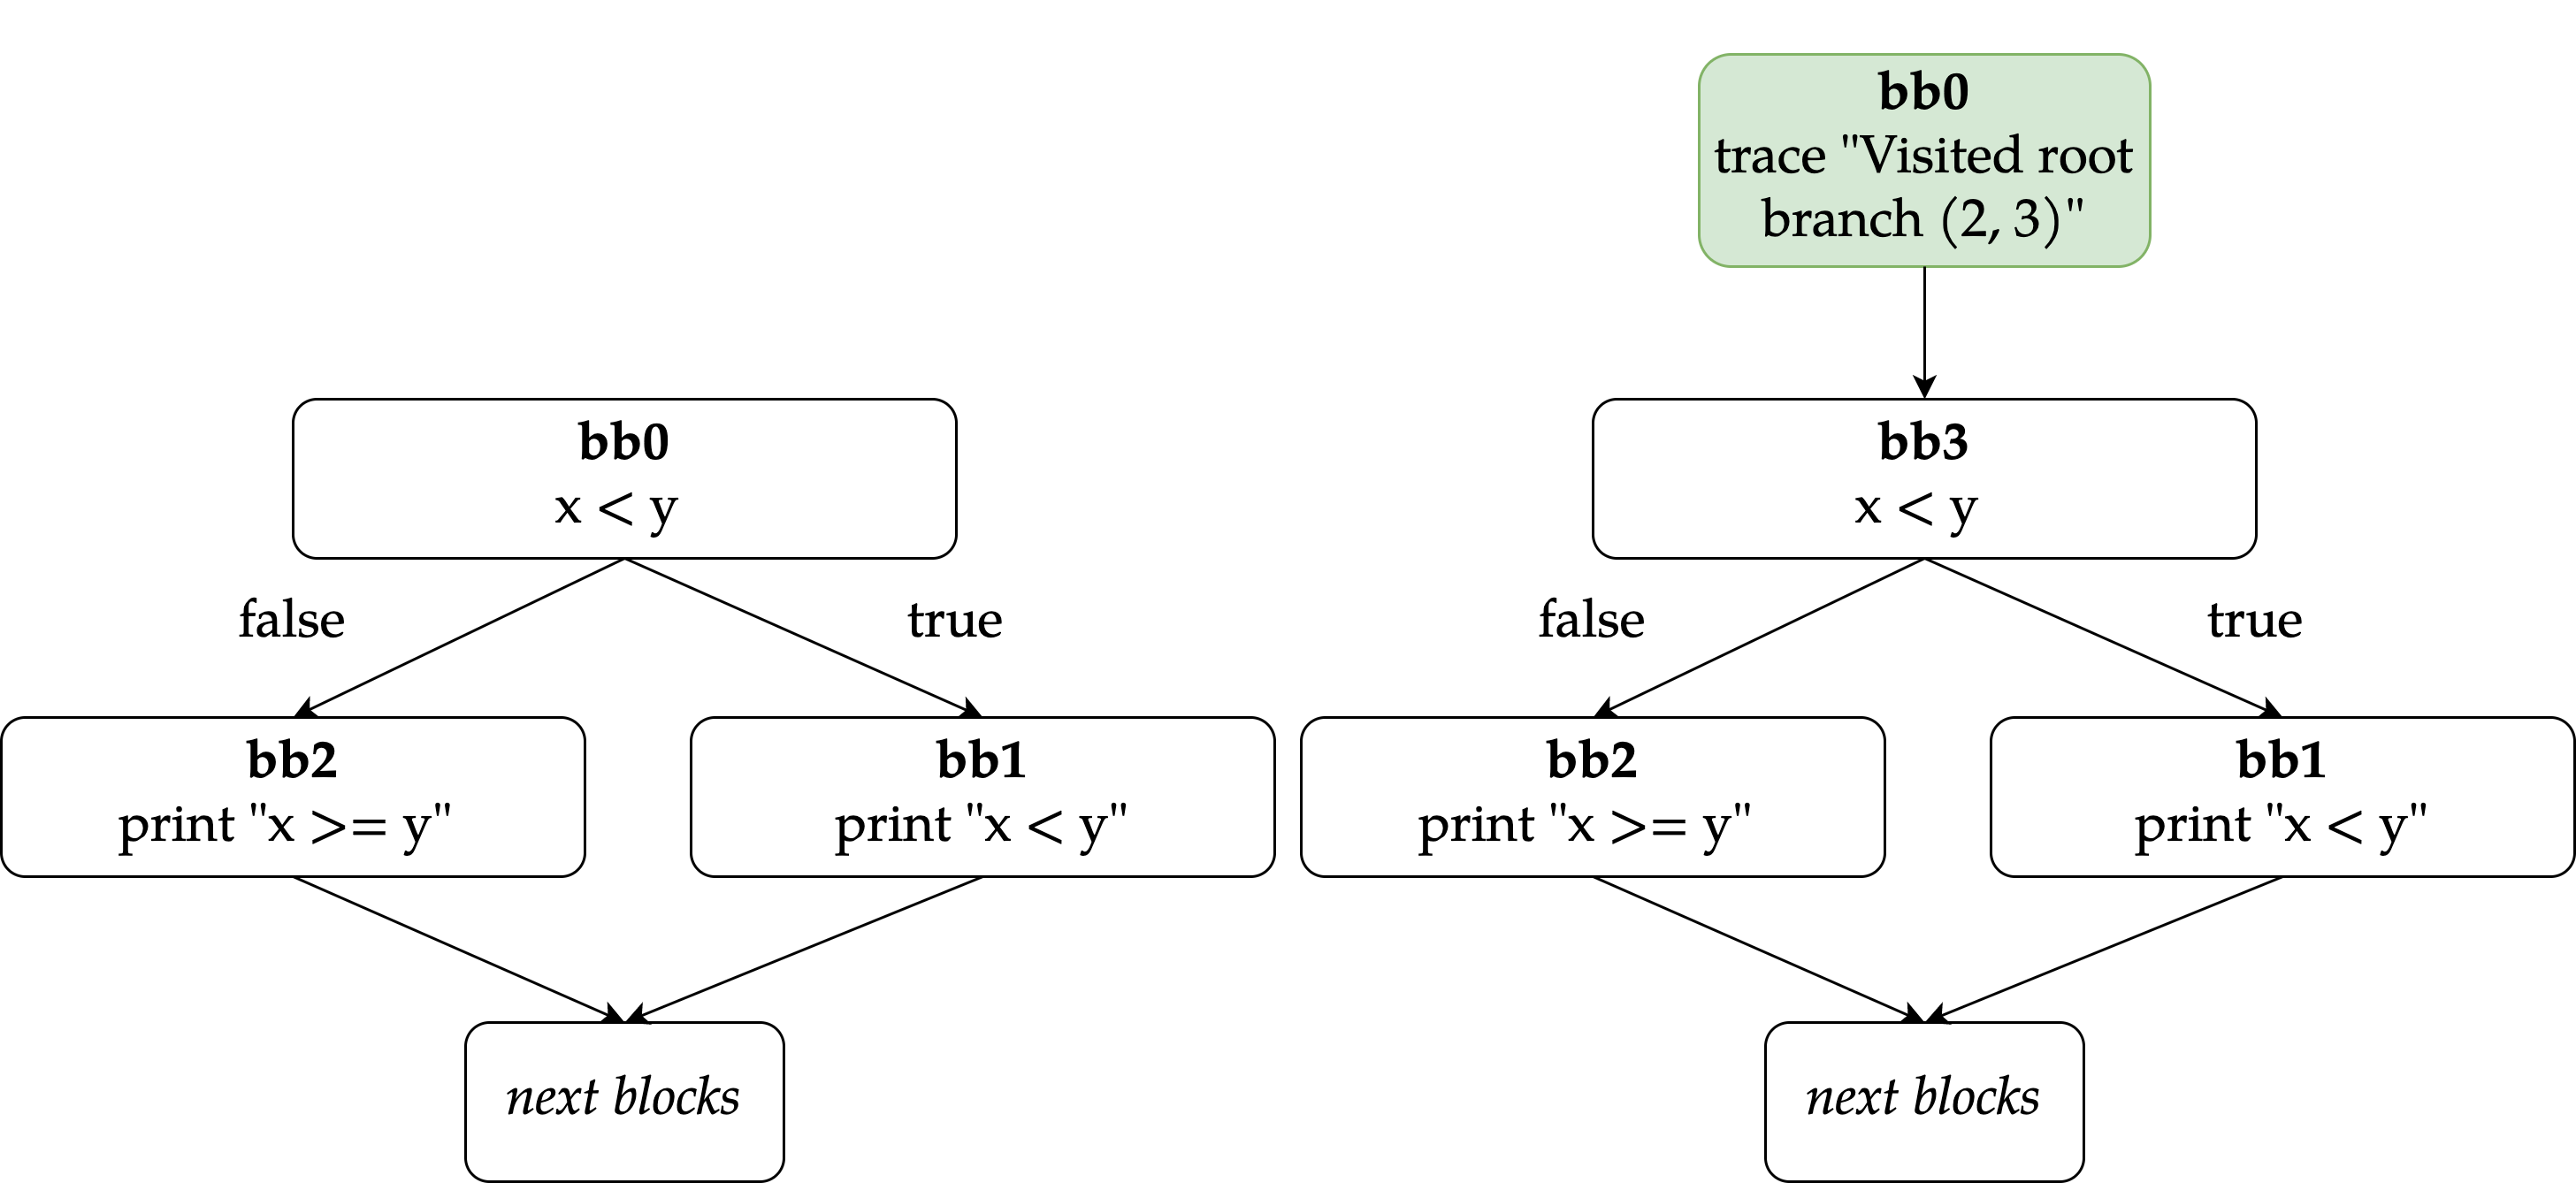
\includegraphics[width=\textwidth]{comparison-instrumented-fn-entry}
\label{fig:comparison-instrumented-fn-entry}
\end{figure}

\subsection{Branch Instrumentation}
To trace the execution of a branch, we need to insert calls to the monitor after a branch has been taken and just before it starts to execute. Doing so, we first update a terminator where branching begins, e.g., \texttt{switchInt}, to point to our artificial tracing blocks. Here, the number of tracing blocks per branch is equal to the number of branches. This is due to the fact that after a particular branch is taken, we want to trace the distance for all branches. This means that for each possible branch a call to the monitor is needed, i.e. a basic block. At this point, we know pretty much on what basis a particular branch is taken and can thus incorporate appropriate logic. Exact values are then inserted and traced at runtime. In the end, we put a chain of tracing blocks with length $l >= 2$ in each branch. Then, the last block of each tracing chain must point to the original target block of the branching terminator. \Cref{lst:mir-instrument-branch} provides an instrumented version of the \mir shown in \Cref{lst:mir-of-example-function-to-instrument}.

\todo{How do we find the exact values to trace in the MIR in the first place?}

\begin{lstlisting}[language={MIR}, style=boxed, caption={Instrumented branches in the \mir of the \texttt{foo} function}, label=lst:mir-instrument-branch]
fn foo(_1: i32, _2: i32) -> () {
  // Locals definition
  // ...
  let mut _11: monitor::BinaryOp;
  let mut _26: monitor::BinaryOp;
  let mut _34: monitor::BinaryOp;
  let mut _40: monitor::BinaryOp;


  @bb0@: {
    _4 = _1;
    _5 = _2;
    _3 = Lt(move _4, move _5);
    switchInt(move _3) -> [false: @bb4@, otherwise: @bb6@];
  }

  @bb2@: {
    // print "x >= y"
  }

  @bb1@: {
    // print "x < y"
  }

  @bb4@: {
    _8 = _1;
    _7 = move _8 as f64 (Misc);
    _10 = _2;
    _9 = move _10 as f64 (Misc);
    discriminant(_11) = 1;
    _6 = monitor::trace_branch_bool(const 2_u64,
                        const 3_u64,
                        const 2_u64,
                        move _7,
                        move _9,
                        move _11,
                        const false) -> @bb5@;
  }

  @bb5@: {
    _23 = _1;
    _22 = move _23 as f64 (Misc);
    _25 = _2;
    _24 = move _25 as f64 (Misc);
    discriminant(_26) = 1;
    _21 = monitor::trace_branch_bool(const 2_u64,
                        const 3_u64,
                        const 1_u64,
                        move _22,
                        move _24,
                        move _26,
                        const true) -> @bb2@;
  }

  @bb6@: {
    _31 = _1;
    _30 = move _31 as f64 (Misc);
    _33 = _2;
    _32 = move _33 as f64 (Misc);
    discriminant(_34) = 1;
    _29 = monitor::trace_branch_bool(const 2_u64,
                        const 3_u64,
                        const 2_u64,
                        move _30,
                        move _32,
                        move _34,
                        const false) -> @bb7@;
  }

  @bb7@: {
    _37 = _1;
    _36 = move _37 as f64 (Misc);
    _39 = _2;
    _38 = move _39 as f64 (Misc);
    discriminant(_40) = 1;
    _35 = monitor::trace_branch_bool(const 2_u64,
                        const 3_u64,
                        const 1_u64,
                        move _36,
                        move _38,
                        move _40,
                        const true) -> @bb1@;
  }

  // Other blocks
}
\end{lstlisting}

In tracing chains (\texttt{bb4}, \texttt{bb5}) and (\texttt{bb6}, \texttt{bb7}) we want to invoke appropriate monitor functions and store all the information we need to identify and compute the branch distance. \Cref{fig:comparison-instrumented-branch-cfg} demonstrates the \cfg of the function before and after instrumentation of its branches. As with \texttt{monitor::trace\string_root} in \Cref{lst:mir-instrument-root}, for each tracing call, we specify the IDs of the module and function, as well as the ID of the branch which the tracing runs within. The branch identificator is usually the number of the block the branching terminator originally pointed to, e.g., in this case we have to branch IDs: $1$ and $2$. We also store the the operands of the binary operation in the \texttt{if} conditional, as well as the binary operation itself. In the end, the polarization of the branches remains, i.e., \texttt{true} or \texttt{false}. With this information we can distinguish in the monitor whether the given branch was hit or not and determine the distance using the values and the binary operation reported. For example, assume that we invoke \texttt{foo(10, 20)} again; then, we get the following trace output:

\begin{lstlisting}[language={}, style=boxed, caption={}, label=lst:mir-instrument-branch-trace-output]
// bb6 gets executed
Distance to branch (2, 3, 2) is 10.0

// bb7 gets executed
Distance to branch (2, 3, 1) is 0.0
\end{lstlisting}

Since $10 < 20$, the execution takes the \texttt{true} branch, i.e., the trace chain of blocks \texttt{bb6} and \texttt{bb7} are run. In \texttt{bb6}, we trace the \texttt{false} branch while the actually executed branch is \texttt{true}. We know that because we can also evaluate the operation \texttt{monitor::BinaryOp::LT} with the operands $10$ and $20$ in the monitor. To calculate the local branch distance, we resort to the formulas in \Cref{tab:local-branch-distance-formulas}.

For reference, \Cref{lst:basic-block-in-regular-rust} shows how the basic block~\texttt{bb4} would look like if it was written in regular Rust.

\begin{lstlisting}[language={}, style=boxed, caption={How would \texttt{bb4} look like in regular Rust code}, label=lst:basic-block-in-regular-rust]
monitor::trace_branch_bool(
  2u64, // module id
  3u64, // function id within the module
  3u64, // branch block id within the function
  x as f64,
  y as f64,
  monitor::BinaryOp::LT,
  false // branch polarization
);
\end{lstlisting}

\begin{figure}[h]
\caption{Instrumentation of regular branches}
\centering
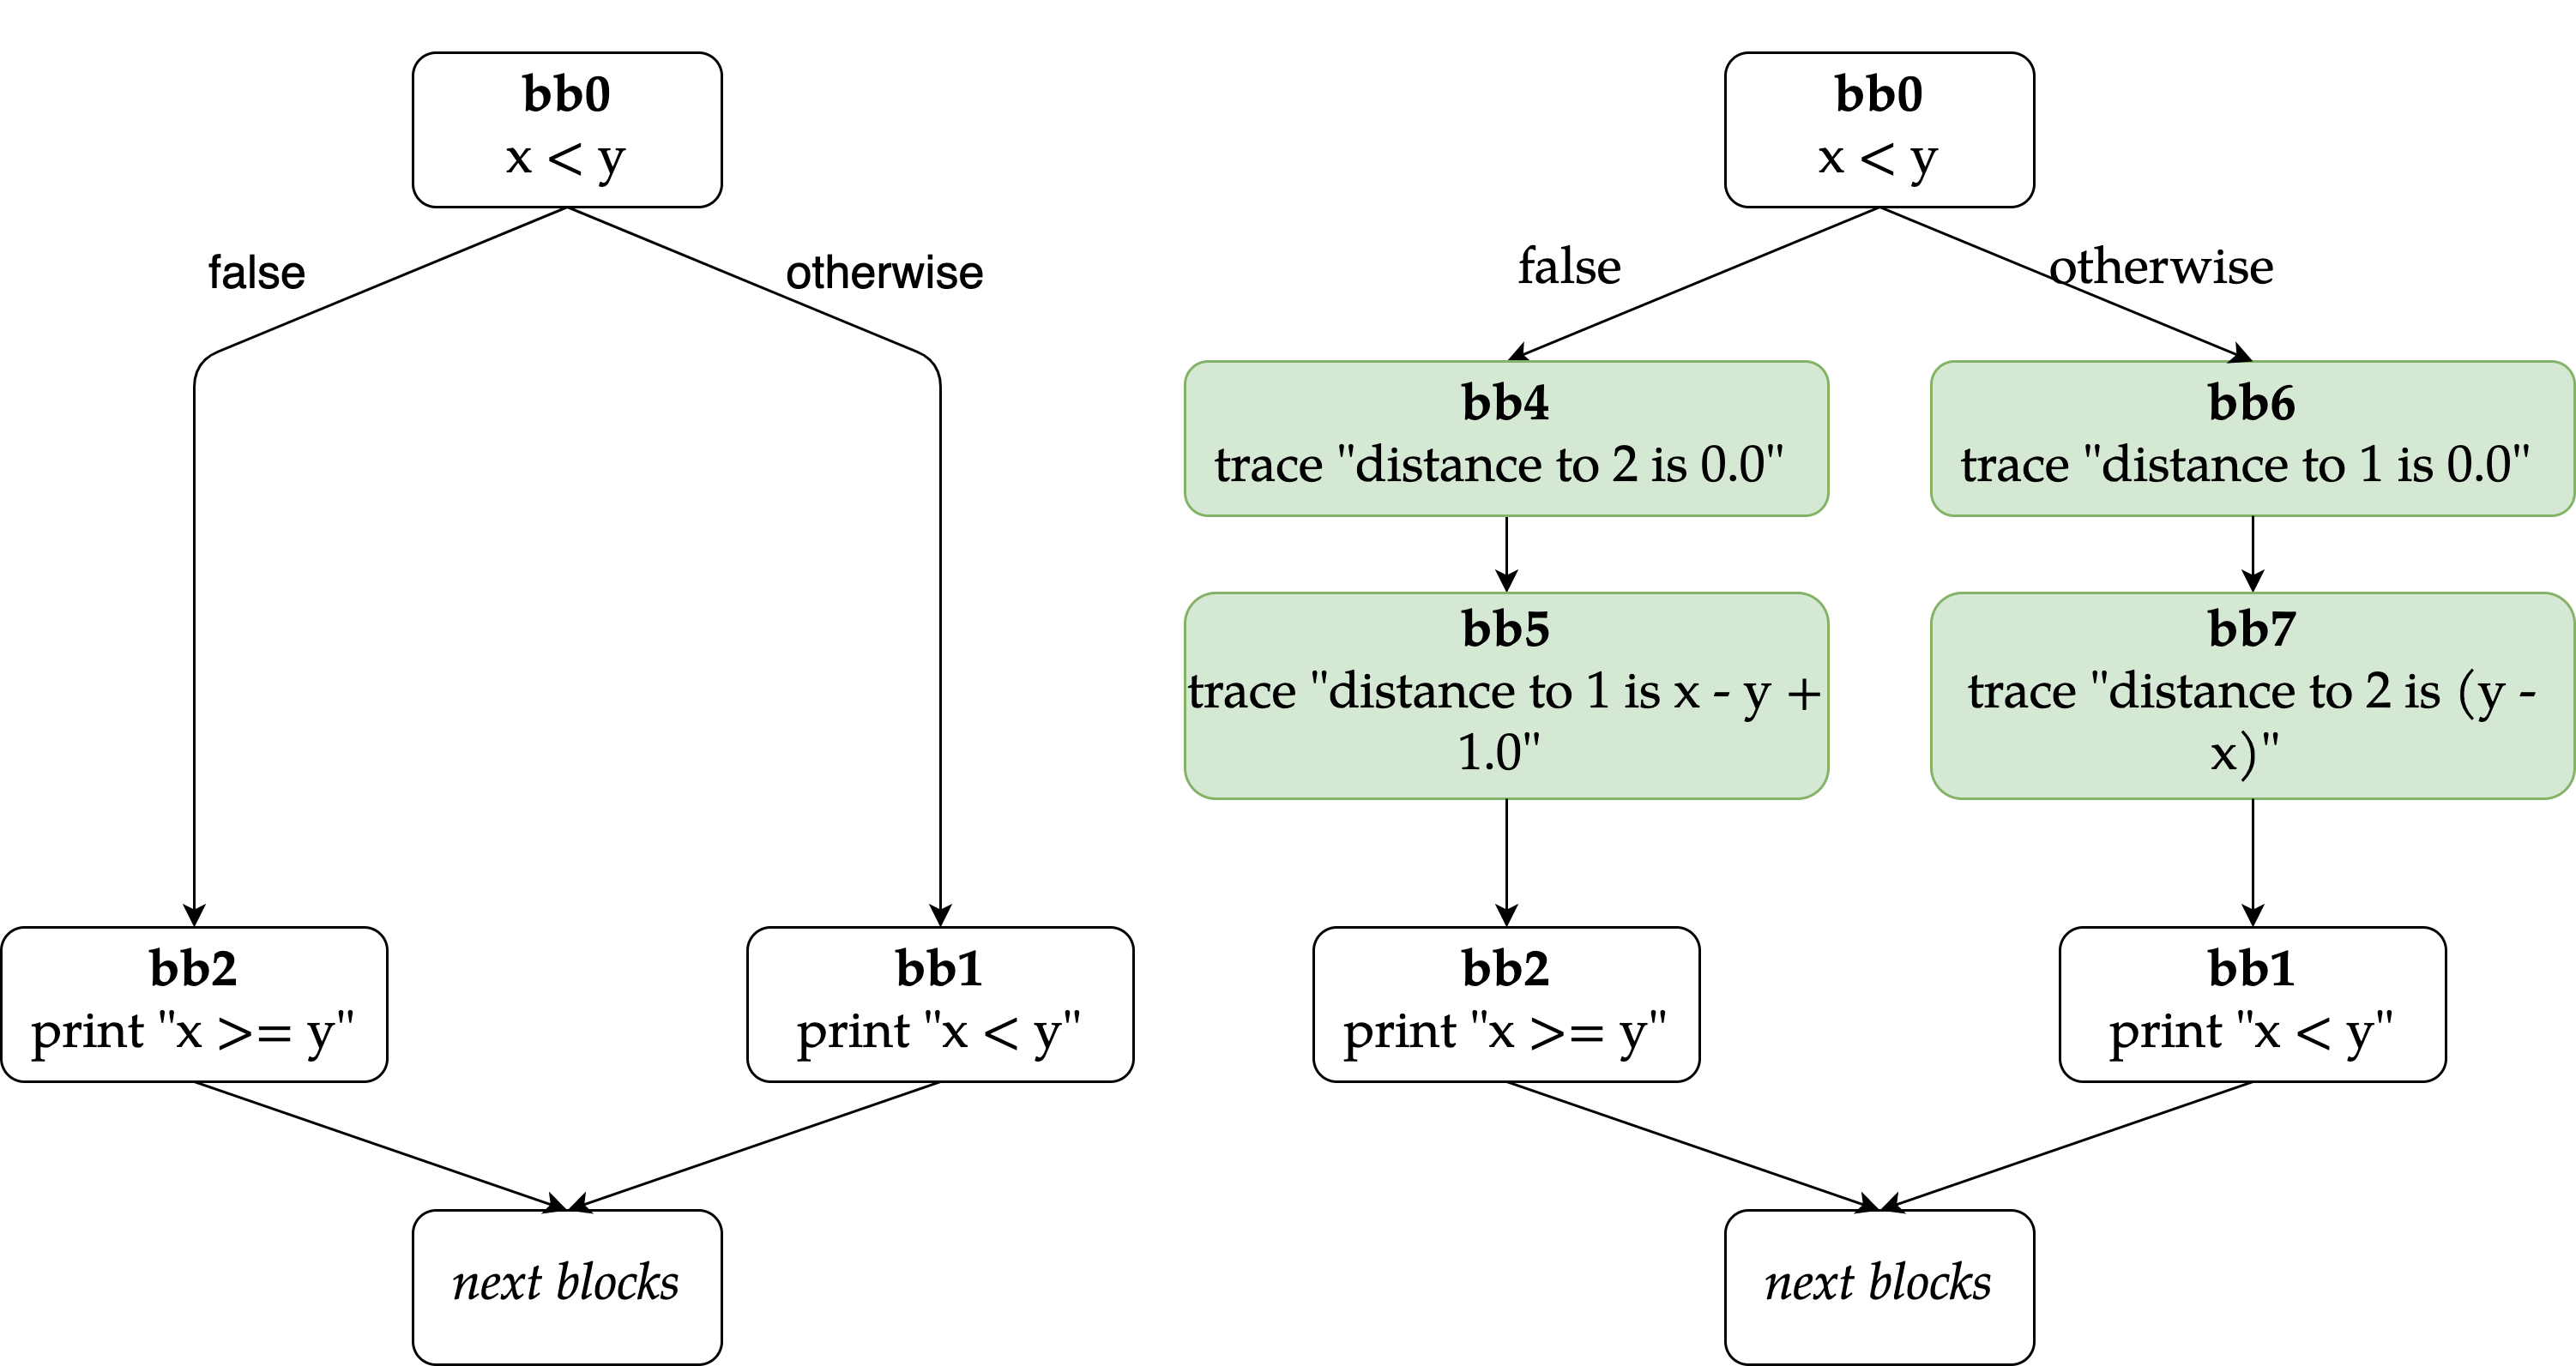
\includegraphics[width=\textwidth]{comparison-instrumented-branch-cfg}
\label{fig:comparison-instrumented-branch-cfg}
\end{figure}

\subsection{Testability Transformation Instrumentation}
\label{sec:mir-testability-transformations}
% TODO reword
In the following, we describe several transformations implemented in the \tech test, some of which were presented by Fraser and Arcuri~\cite{Fraser2013} for the \textsc{EvoSuite} tool. The transformations are implemented at the \mir level. To do so, we need to introduce additional tracing blocks at crucial points. The Rust compiler transforms input programs in the same way as it is done with testability transformations, which are described in~\Cref{sec:testability-transformations}. It inserts assertions at relevant places to check for unexpected behavior, for instance, whether an index is within an array's bounds or an arithmetic operation results in overflow.

Accessing an array with an inappropriate index results in a program crash. This happens because the compiler inserts checks before each array access that shall verify whether a given index is within the bounds of the array. If not, the program panics. Assume the following function that takes an index and an \texttt{i32}-array of size~$3$ and returns the value at the given position:
\begin{lstlisting}[style=boxed, caption={}, label=lst:array-index-access-example]
fn get(pos: usize, array: &[i32; 3]) -> i32 {
  array[pos]
}
\end{lstlisting}

\Cref{lst:mir-boundary-check} shows the relevant part of its \mir. Before the block that accesses the array (Line~\ref{line:array-access}), the compiler inserted an assertion in~Line~\ref{line:array-index-assertion} that checks whether the index is less than the length of the array, which is a static constant. If the index is greater than or equal to the length, the program crashes. The other case, i.e., negative index, cannot occur since its value must always be of type \texttt{usize}, i.e. an unsigned type, which is guaranteed by the compiler again. Thus, there is no reason to verify this case.

\begin{lstlisting}[language={MIR}, style=boxed, escapechar=§, caption={Compiler inserts runtime assertions at places where arrays are accessed by index}, label=lst:mir-boundary-check]
fn get(_1: usize, _2: &[i32; 3]) -> i32 {
  // Locals  definition

  @bb0@: {
    _3 = _1;
    _4 = const 3_usize;
    _5 = Lt(_3, _4);
    assert(move _5, §\label{line:array-index-assertion}§
        "index out of bounds:
          the length is {} but the index is {}",
        move _4,
        _3) -> @bb1@;
  }

  @bb1@: {
    _0 = (*_2)[_3]; §\label{line:array-access}§
    return;
  }
}
\end{lstlisting}

That is, the compiler inserts an assertion that checks whether the index is less than the length of the array, which is statically constant. If the index is greater than or equal to the length, the program crashes. The other case, i.e. negative index, cannot occur since the index must always be of type \texttt{usize}, i.e. an unsigned type. Thus, there is no reason to verify this case.

Now, we need to insert tracing blocks for both, the ``good'' and the ``bad'' case. We could insert two branches always before an assertion block. However, in this case we would have to insert another branching block $s$, for example with \texttt{switchInt}, and if applicable we would have to change the original preceding assertion block so that it points to $s$. In the block $s$ we would also have to copy the logic from the assertion block, which makes the whole thing even more complicated. Another option would be to change the assertion itself. An assertion in \mir has an optional unwind edge which, in the "bad" case, points to a sequence of blocks to clean up before the program crashes, if there is anything to clean up. Assume the function \texttt{get} from \Cref{lst:array-index-access-example} does some allocations before accessing the array:
\begin{lstlisting}[style=boxed, caption={}]
fn get(pos: usize, array: &[i32; 3]) -> i32 {
  let s = String::from("I'm using heap");
  array[pos]
}
\end{lstlisting}

Then, the the \mir of the function becomes a bit different:
\begin{lstlisting}[language={MIR}, style=boxed, caption={}, label=lst:mir-boundary-check-with-unwinding]
fn get(_1: usize, _2: &[i32; 3]) -> i32 {
  // Locals  definition
  @bb0@: {
    _3 = <String as From<&str>>::from(
      const "I'm using heap"
    ) -> @bb1@;
  }

  @bb1@: {
    _4 = _1;
    _5 = const 3_usize;
    _6 = Lt(_4, _5);
    assert(move _6,
      "index out of bounds:
        the length is {} but the index is {}",
      move _5,
      _4
    ) -> [success: @bb2@, unwind: @bb4@];
  }

  @bb2@: {
    _0 = (*_2)[_4];
    // Drop the string
    drop(_3) -> @bb3@;
  }

  @bb3@: {
      return;
  }

  @bb4@ (cleanup): {
    // Drop the string
    drop(_3) -> @bb5@;
  }

  // Other blocks
}
\end{lstlisting}

The assertion has now got a second edge. Regardless of whether the index is valid or not, the string will be cleaned up in any case. The behavior is similar to the \texttt{finally} block from the \texttt{try-catch} construct in Java. We exploit the unwind edge of assertions: if an assertion has an unwind edge, \tech inserts the tracing chain between the assertion and and the existing cleanup blocks. Otherwise, we create an unwind edge manually and connect it to the tracing chain. The instrumentation of assertions is illustrated in~\Cref{fig:comparison-instrumented-assertion}. Since there are two branches, \tech adds a tracing chain of two tracing blocks to each branch. So in case the index is not valid, we the executed path is traced as usual before the proram exits. Thus, we know that the respective test has covered the path. In addition, we get a guidance for the two possible cases.

\begin{figure}[h]
\caption{Instrumented assertion}
\centering
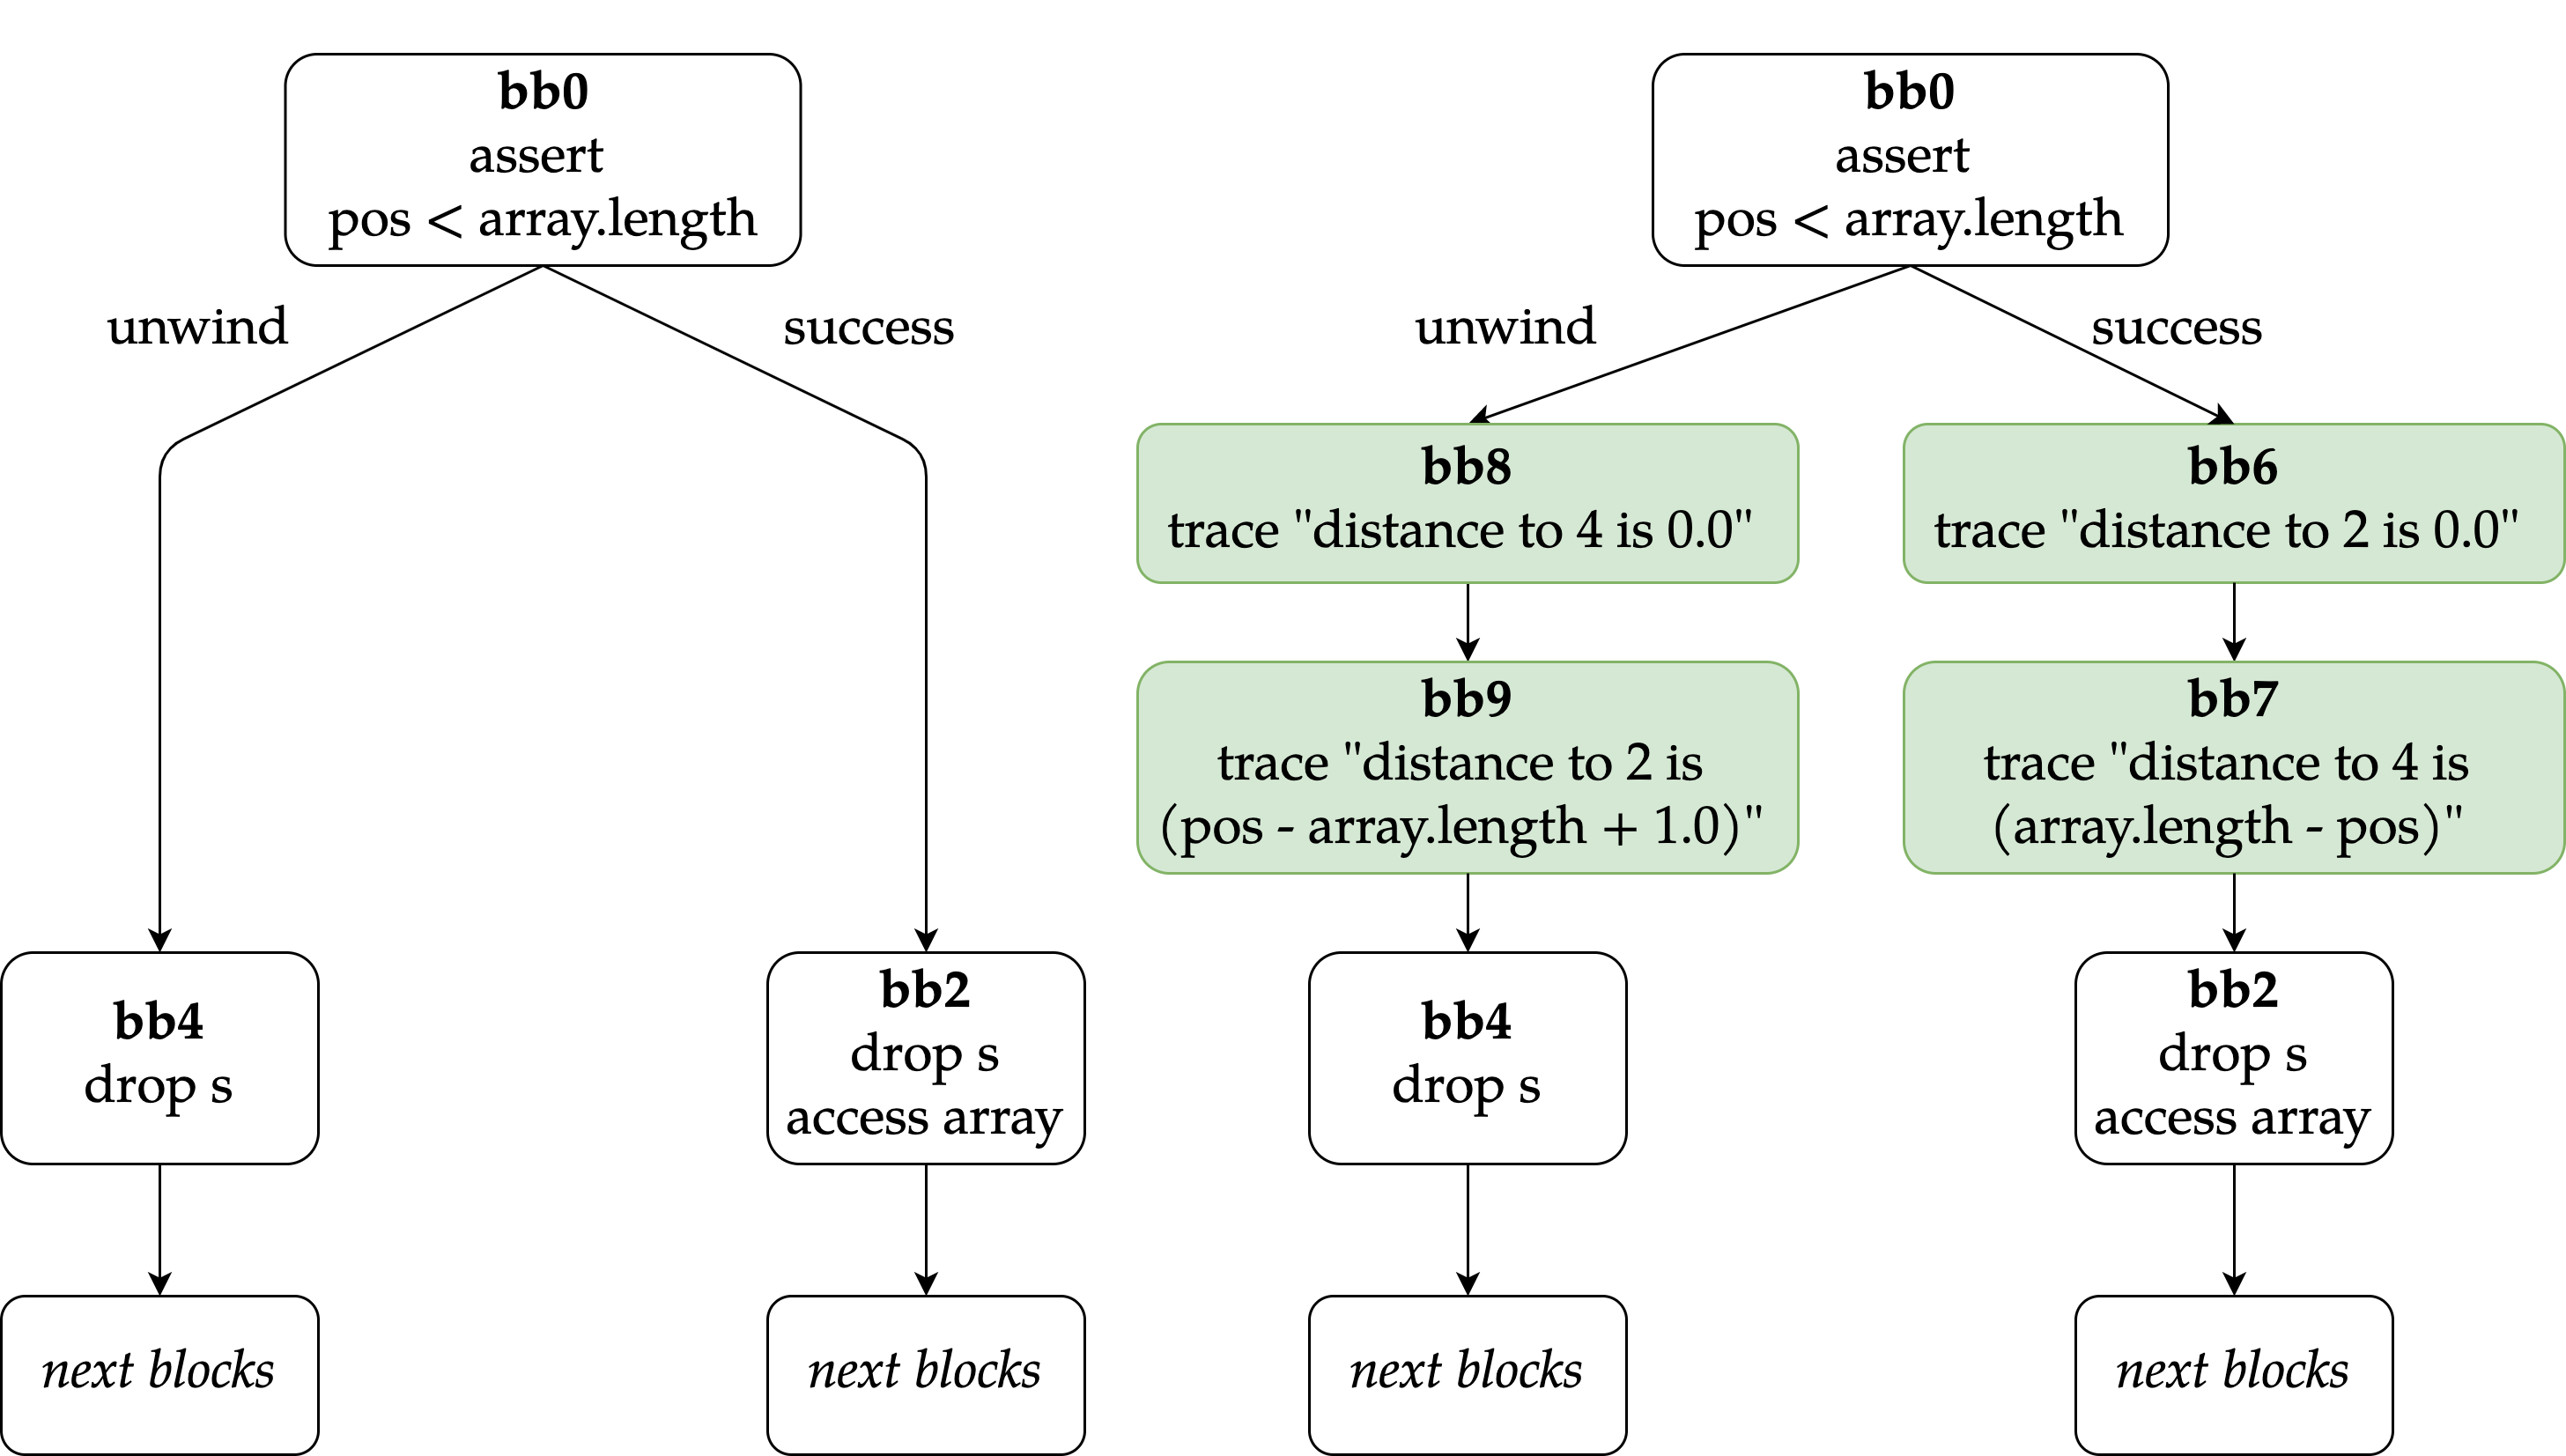
\includegraphics[width=\textwidth]{comparison-instrumented-assertion}
\label{fig:comparison-instrumented-assertion}
\end{figure}

We do the same for the case of overflows and underflows. \Cref{lst:mir-overflow-check} demonstrates an example of the \texttt{add} function that performs addition of two eight-bit integers and the relevant basic block from its \mir. In its \mir, the compiler inserts an assertion about the value of the result to catch a possible overflow. \tech instruments the assertion and insert our tracing chains into the body of the function as described above.
% OVERFLOW CHECK
\begin{lstlisting}[language={MIR}, style=boxed, caption={\mir overflow check created by the compiler}, label=lst:mir-overflow-check]
fn add(a: i8, b: i8) -> i8 {
  a + b
}

@bb0@: {
  _3 = _1;
  _4 = _2;
  _5 = CheckedAdd(_3, _4);
  assert(
    !move (_5.1: bool),
    "attempt to compute `{} + {}`,
      which would overflow",
    move _3,
    move _4
  ) -> @bb1@;
}
\end{lstlisting}

\section{Handling Generics and Traits}
A large part of \ac{SBST} approaches is applied to managed languages such as Java, since these offer a rich set of tools and features like reflection. Reflection allows to analyze the code of the \sut and extract information needed for generating tests by querying the appropriate language \ac{API}, like \texttt{getGenericParameters} of a \texttt{java.lang.reflect.Method} instance to get generic parameters. However, when tests are generated for generic elements, it is sometimes difficult to replace a generic type parameter with a matching concrete type because execution depends on the one concrete type~\cite{Fraser2014b}. As shown in \Cref{lst:java-isinstanceof}, an execution path for generic methods can be affected by checks for the concrete type of a generic instance. Many approaches to analyzing Java programs operate at the bytecode level after type erasure has already happened. This means that bytecode does not know anything about generics, they are replaced, for example, by \texttt{Object}.

\begin{lstlisting}[language=Java, style=boxed, caption={The execution path of the generic Java method depends on the concrete type of the argument}, label=lst:java-isinstanceof]
public class GenericsExample<T, K> {
  public int typedInput(T value) {
    if (value isinstanceof String) {
      return 0;
    } else if (value isinstanceof Integer) {
      return 1;
    } else if (value isinstanceof Double) {
      return 2;
    } else {
      return 3;
    }
  }
}
\end{lstlisting}

Similar approach is also possible in Rust to find out the concrete type of a generic, as shown in~\Cref{lst:rust-runtime-reflection}. A crucial requirement of this is the conversion of the generic type to \texttt{dyn Any}. Then, we can check the runtime type of \texttt{value}. The downcasts are also part of \mir and thus can theoretically be used to determine possible suitable types for a generic to narrow down the space of possible types. However, since generics with trait bounds are often a more suitable option, this feature is quite rare and cannot be found in the evaluation subjects, which makes us rely on a more general approach.

\begin{lstlisting}[style=boxed, caption={The execution path of the generic Rust function depends on the concrete type of the argument}, label=lst:rust-runtime-reflection]
use std::fmt::Debug;
use std::any::Any;

fn typed_input<T: Any>(value: &T) -> i32 {
  let value_any = value as &dyn Any;

  if let Some(as_string)
      = value_any.downcast_ref::<String>() {
    return 0;
  } else if let Some(as_int)
      = value_any.downcast_ref::<i32>() {
    return 1;
  } else if let Some(as_double)
      = value_any.downcast_ref::<f64>() {
    return 2;
  } else {
    return 3;
  }
}
\end{lstlisting}

Whenever \tech needs to bind a generic type parameter with an actual one, it applies \Cref{alg:get-necessary-bindings}. The algorithm returns a type binding, which is a mapping from generic to actual types. Assume that we want to know how the type parameters \emph{T} and \emph{E} should be replaced in \texttt{Result<Box<T>, E>} to get a \texttt{Result<Box<MyType>, MyError>}. \Cref{alg:get-necessary-bindings} starts from the most outer type, i.e., \texttt{Result}. Since the given type is not a type parameter and also not a reference, the algorithm unwraps the generics of the outer type and recursively tries to map \texttt{Box<T>} to \texttt{Box<MyType>} and \texttt{E} to \texttt{Error}. \texttt{E} is a type parameter, so we store the binding \texttt{\string{E -> Error\string}}. \texttt{Box} is a not a type parameter and not a reference either. In the last step, the algorithm stores the additional binding \texttt{\string{T -> MyType\string}}.

\begin{algorithm}[t]
  \caption{$GetNecessaryBindings(G, C, T)$}\label{alg:get-necessary-bindings}
\begin{algorithmic}
\Input
  \Desc{$G$}{A generic type}
  \Desc{$C$}{A concrete type}
  \Desc{$T$}{Type binding}
\EndInput

\If{$G$ is a type parameter}
\State $T[G] \gets C$
\Else
  \If{$G$ is a reference and $C$ is a reference}
    \State $G_r \gets $ referenced type of $G$
    \State $C_r \gets $ referenced type of $C$
    \State $GetNecessaryBindings(G_r, C_r, T)$
  \Else
    \State $I_g \gets $ inner generics of $G$
    \State $I_c \gets $ inner generics of $C$
    \State $n \gets \left| I_g \right|$
    \For{$i \in (1, n)$}
      \State $GetNecessaryBindings(I_g[i], I_c[i], T)$
    \EndFor
  \EndIf
\EndIf
\end{algorithmic}
\end{algorithm}

% TODO reword
The problem of generics becomes relevant whenever the test generation algorithm attempts to instantiate a new instance of a generic type, or to satisfy a parameter for a newly inserted method call. Assume that our test generation algorithm decides to add a call to the method \texttt{get(self: \&Foo<T>)} of the struct \texttt{Foo<T>}, which is defined and implemented as follows:
\begin{lstlisting}[style=boxed, caption={}, label=lst:basic-generics-example]
struct Foo<T> {
  bar: T
}

impl<T> for Foo<T> {
  fn new(bar: T) -> Self {
    Self { bar }
  }

  fn get(&self) -> Option<T> {
    // ...
  }

  fn update(&mut self, bar: T) {
    // ...
  }
}
\end{lstlisting}

From the \hir analysis we know that \texttt{T} is a type parameter of the struct and is not bound by any other constraints. This means that \tech can freely replace \texttt{T} by any type in that case. To keep the testing effort smaller, we always check first whether we can fill a generic type parameter by a primitive type from the standard library, if the constraints allow this. Here, for instance, the algorithm could choose \emph{isize} as a good candidate.

The strategy is to first determine the return type of the selected method and then create the potentially necessary dependencies backwards based on that. That is, we invoke \texttt{Foo::get(\&self)} and store the return value into a variable of type \texttt{Option<isize>}. We obtain a type binding $TB$ with \texttt{GetNecessaryBindings(Option<T>, Option<isize>, TB)}. The binding \texttt{\string{T -> isize\string}} between the generic type parameter and the concrete type is stored for the variable for later use.

\begin{lstlisting}[style=boxed, caption={}, label=lst:building-generic-test-1]
#[test]
fn rusty_test_0() {
  let mut option_0: Option<isize> = Foo::get(&foo_0);
}
\end{lstlisting}
The test is not compilable as is, though. This is why we use \texttt{GenObject} to create an instance of \texttt{Foo}, e.g., by invoking its constructor. The constructor has a parameter of type \texttt{T} which we already have a binding for; it effectively makes us able to call the constructor with a random integer: %as shown in~\Cref{lst:building-generic-test-2}.
\begin{lstlisting}[style=boxed, caption={}, label=lst:building-generic-test-2]
#[test]
fn rusty_test_0() {
  let mut isize_0 = 42isize;
  let mut foo_0: Foo<isize> = Foo::new(isize_0);
  let mut option_0: Option<isize> = Foo::get(&foo_0);
}
\end{lstlisting}
%For example, another method call, e.g., \texttt{update(\string&mut self, bar: T)}, can be generated on the \texttt{Foo} instance. For the call, the appropriate argument must be generated first. It is already known that the variable \texttt{foo\string_0} has the type \texttt{Foo<isize>} and thus, maps \texttt{T} to \texttt{isize}. Using this knowledge base, the algorithm generates two more statements as follows:



% Generics Mixup Beispiel: https://doc.rust-lang.org/book/ch10-01-syntax.html

%Listing~\ref{lst:java-interface-example} shows the function \texttt{area} that accepts objects of type \texttt{Shape}, that is, instances of classes that implement the interface. To test the \texttt{area} function, one would have to find a type that implements the interface. Reflection can be used to query classes that do. This is possible because Java runs in a virtual machine that carries this information.

%\begin{lstlisting}[language=Java, style=boxed, caption={A function that takes objects implementing an interface}, label=lst:java-interface-example]
%public interface Shape {
%    double area();
%}
%
%public class Rectangle implements Shape {
%  private double length;
%  private double height;
%
%  @Override
%  public double area() {
%      return length * height;
%  }
%}
%
%public class Main {
%    public static double area(Shape shape) {
%        return shape.area();
%    }
%}
%\end{lstlisting}


Generics play a very important role in Rust. It is not a typical object-oriented language and instead of using direct types, for example as method parameters, as is often the case in Java, generics are rather used in conjunction with trait bounds. Trait bounds define what behavior a particular generic type must be capable of. This reduces the number of possible data types a type parameter can be filled with. \Cref{lst:trait-bounds-example} implements the \texttt{area} function in Rust, which takes a parameter of generic type~\texttt{T}. The type parameter \texttt{T} must implement the \texttt{HasArea} trait, which allows \texttt{area} to access the trait's functions. %Unlike Java, there is only a very limited runtime reflection provided in Rust and boils down to the example shown in~\Cref{lst:rust-runtime-reflection}. The Rust compiler compiler the source code into machine executable code, and all superfluous information is eliminated during the compilation process.

\begin{lstlisting}[style=boxed, caption={A function that takes a generic types and specifies a bound}, label=lst:trait-bounds-example]
trait HasArea {
  fn area(&self) -> f64;
}

struct Rectangle { length: f64, height: f64 }

impl HasArea for Rectangle {
  fn area(&self) -> f64 { self.length * self.height }
}

// `T` must implement `HasArea`. Any type which meets
// the bound can access `HasArea`'s function `area`.
fn area<T: HasArea>(t: &T) -> f64 { t.area() }
\end{lstlisting}

Types that implement a particular trait must thus be found statically during compilation of the \sut and annotated. The compiler provides \acp{API} to query all traits and the collection of the respective \texttt{impl} blocks, not only in the compiled \sut, but also in its dependencies and in the standard library itself, as shown in \Cref{lst:query-types-that-implement-trait}. Each \texttt{impl} block associate with a specific type, i.e., struct or enum. Thus, we can transitively learn if a type implements a certain trait.

\begin{lstlisting}[style=boxed, caption={Query types for a trait}, label=lst:query-types-that-implement-trait]
fn get_types_for_trait(trait_id: DefId,
    tcx: &TyCtxt<'_>) -> Vec<Type> {
  let trait_impls = tcx.trait_impls_of(trait_id);
  let types = trait_impls.iter()
    .map(|im| tcx.type_of(im))
    .collect::<Vec<_>>();

  // TODO substitue blanket implementations
}
\end{lstlisting}

Things get more complicated when a trait is generic because it can be implemented multiple times for the same type with different values of the type parameters. ~\Cref{lst:from-trait-example} demonstrates an example implementation of the \texttt{std::convert::From} trait for the type \texttt{MyInt} with a 32-bit integer and a string. Due to the increasing complexity of handling generic traits, \tech can only analyze simple cases, i.e. implementations of non-generic traits, while ignoring the rest.

\begin{lstlisting}[style=boxed, caption={Example implementation oft the std::convert::From trait from the Rust standard library}, label=lst:from-trait-example]
pub trait From<T> {
  fn from(T) -> Self;
}

struct MyInt {
  value: i32
}

impl From<i32> for MyInt {
  fn from(x: i32) -> MyInt {
    MyInt { value: x }
  }
}

impl From<String> for MyInt {
  fn from(s: String) -> MyInt {
    let value = s.parse::<i32>().unwrap();
    MyInt { value }
  }
}
\end{lstlisting}

%However, finding all possible types implementing a particular trait which is not defined in the \sut itself is difficult. Rust compiler proceeds similarly to C++ compiler when compiling: crates are compiled individually and independently and only then, for example, linked with the standard library. However, the \sut from which the build process was started is always compiled last after all dependencies. Thus, all information is available at the time when \tech performs the analysis.

In general, we mainly use primitive data types for a \sut to keep the generated tests simple as far as this satisfies the defined trait bounds. To create a call to the example method \texttt{FooBar::foo} (\Cref{lst:generic-type-used-in-multiple-params}) in a generated test, we would do the following:

\begin{lstlisting}[style=boxed, caption={A generic type A is used in multiple parameters and return value}, label=lst:generic-type-used-in-multiple-params]
struct FooBar<A> {
  // ...
}

impl<A> for FooBar<A> {
  fn new() -> Self {
    // ...
  }

  fn foo(&self, x: A, v: &Vec<A>) -> Option<A> {
    // ...
  }
}
\end{lstlisting}

\begin{enumerate}
    \item Look for a type that satisfies \texttt{A}; \texttt{A} has no bounds, so bind it to a primitive type, e.g., \texttt{i32}. Now, with that information, we know that the parameters \texttt{\string&self}, \texttt{x}, and \texttt{v} have to be of type \texttt{FooBar<i32>}, \texttt{i32}, and \texttt{Vec<i32>}, respectively.
    \item Using \texttt{GenObject} we find that an instance of \texttt{FooBar<A>} can be created by the constructor \texttt{FooBar::new()}, thus, we define \texttt{let f: FooBar<i32> = FooBar::new();}.
    \item Generating a primitive like \texttt{i32} is just a matter of defining some random value, like \texttt{let x: i32 = 42i32;}.
    \item Using \texttt{GenObject}, find a generator that returns a \texttt{Vec<i32>} or a \texttt{Vec<T>} with some generic type \texttt{T}.
    \item From our custom type definition, we know that \texttt{Vec::new()} returns a \texttt{Vec<T>}. We need its inner elements to be of type \texttt{i32}, which does satisfy the generic type \texttt{T}, so we take it and define \texttt{let v: Vec<i32> = Vec::new();}.
    \item Now, we can use the defined variables to generate a call to the \texttt{FooBar::foo} and store its returning value, whose bound type we are aware of, too, as shown in \Cref{lst:example-generated-test}.
\end{enumerate}

\begin{lstlisting}[style=boxed, caption={An example test that invokes \texttt{FooBar::foo}}, label=lst:example-generated-test]
#[test]
fn rusty_test_0() {
  let foobar_0: FooBar<i32> = FooBar::new();
  let i32_0: i32 = 42i32;
  let vec_0: Vec<i32> = Vec::new();
  let option_0: Option<i32> = FooBar::foo(
    &foobar_0, i32_0, &vec_0
  );
}
\end{lstlisting}

\section{Test Execution}
With Cargo, Rust provides a build system and a testing framework out-of-the-box. In Java, which is a managed language~\cite{Gough2005}, generated tests can be executed directly using Reflection and bytecode instrumentation, and coverage information can be collected in the same runtime process. In Rust, we need to run the tests ``traditionally'', i.e., synthesize them into Rust source code, write into the approapriate source file of the \sut, compile, and execute. Due to incremental compilation, rustc generally only needs to recompile the changed test modules. Nevertheless, this introduces a non-negligible overhead that \tech tries to minimize by compiling all tests in a population at once and concurrently executing them.

Cargo's test framework is called on the \sut to run the tests; it does so in parallel by default. To establish the mapping between each individual test and the corresponding execution traces, each test sets a \texttt{thread\string_local} ID at the beginning of its execution, which the instrumentation instructions exploit to report the correct ``author'' of coverage data.

As shown in~\Cref{fig:test-execution}, an instrumented \sut reports important events during its execution to \tech's monitor. Those are, for example, an entrance of a function or an execution of a decision branch. For the latter, the branch distance calculated on-the-fly is passed along with other data. \tech's monitor is initialized before the test threads are started and can either write collected traces to files or to the Redis in-memory storage.

\begin{figure}[h]
\caption{An example concurrent execution of multiple tests with a monitor}
\centering
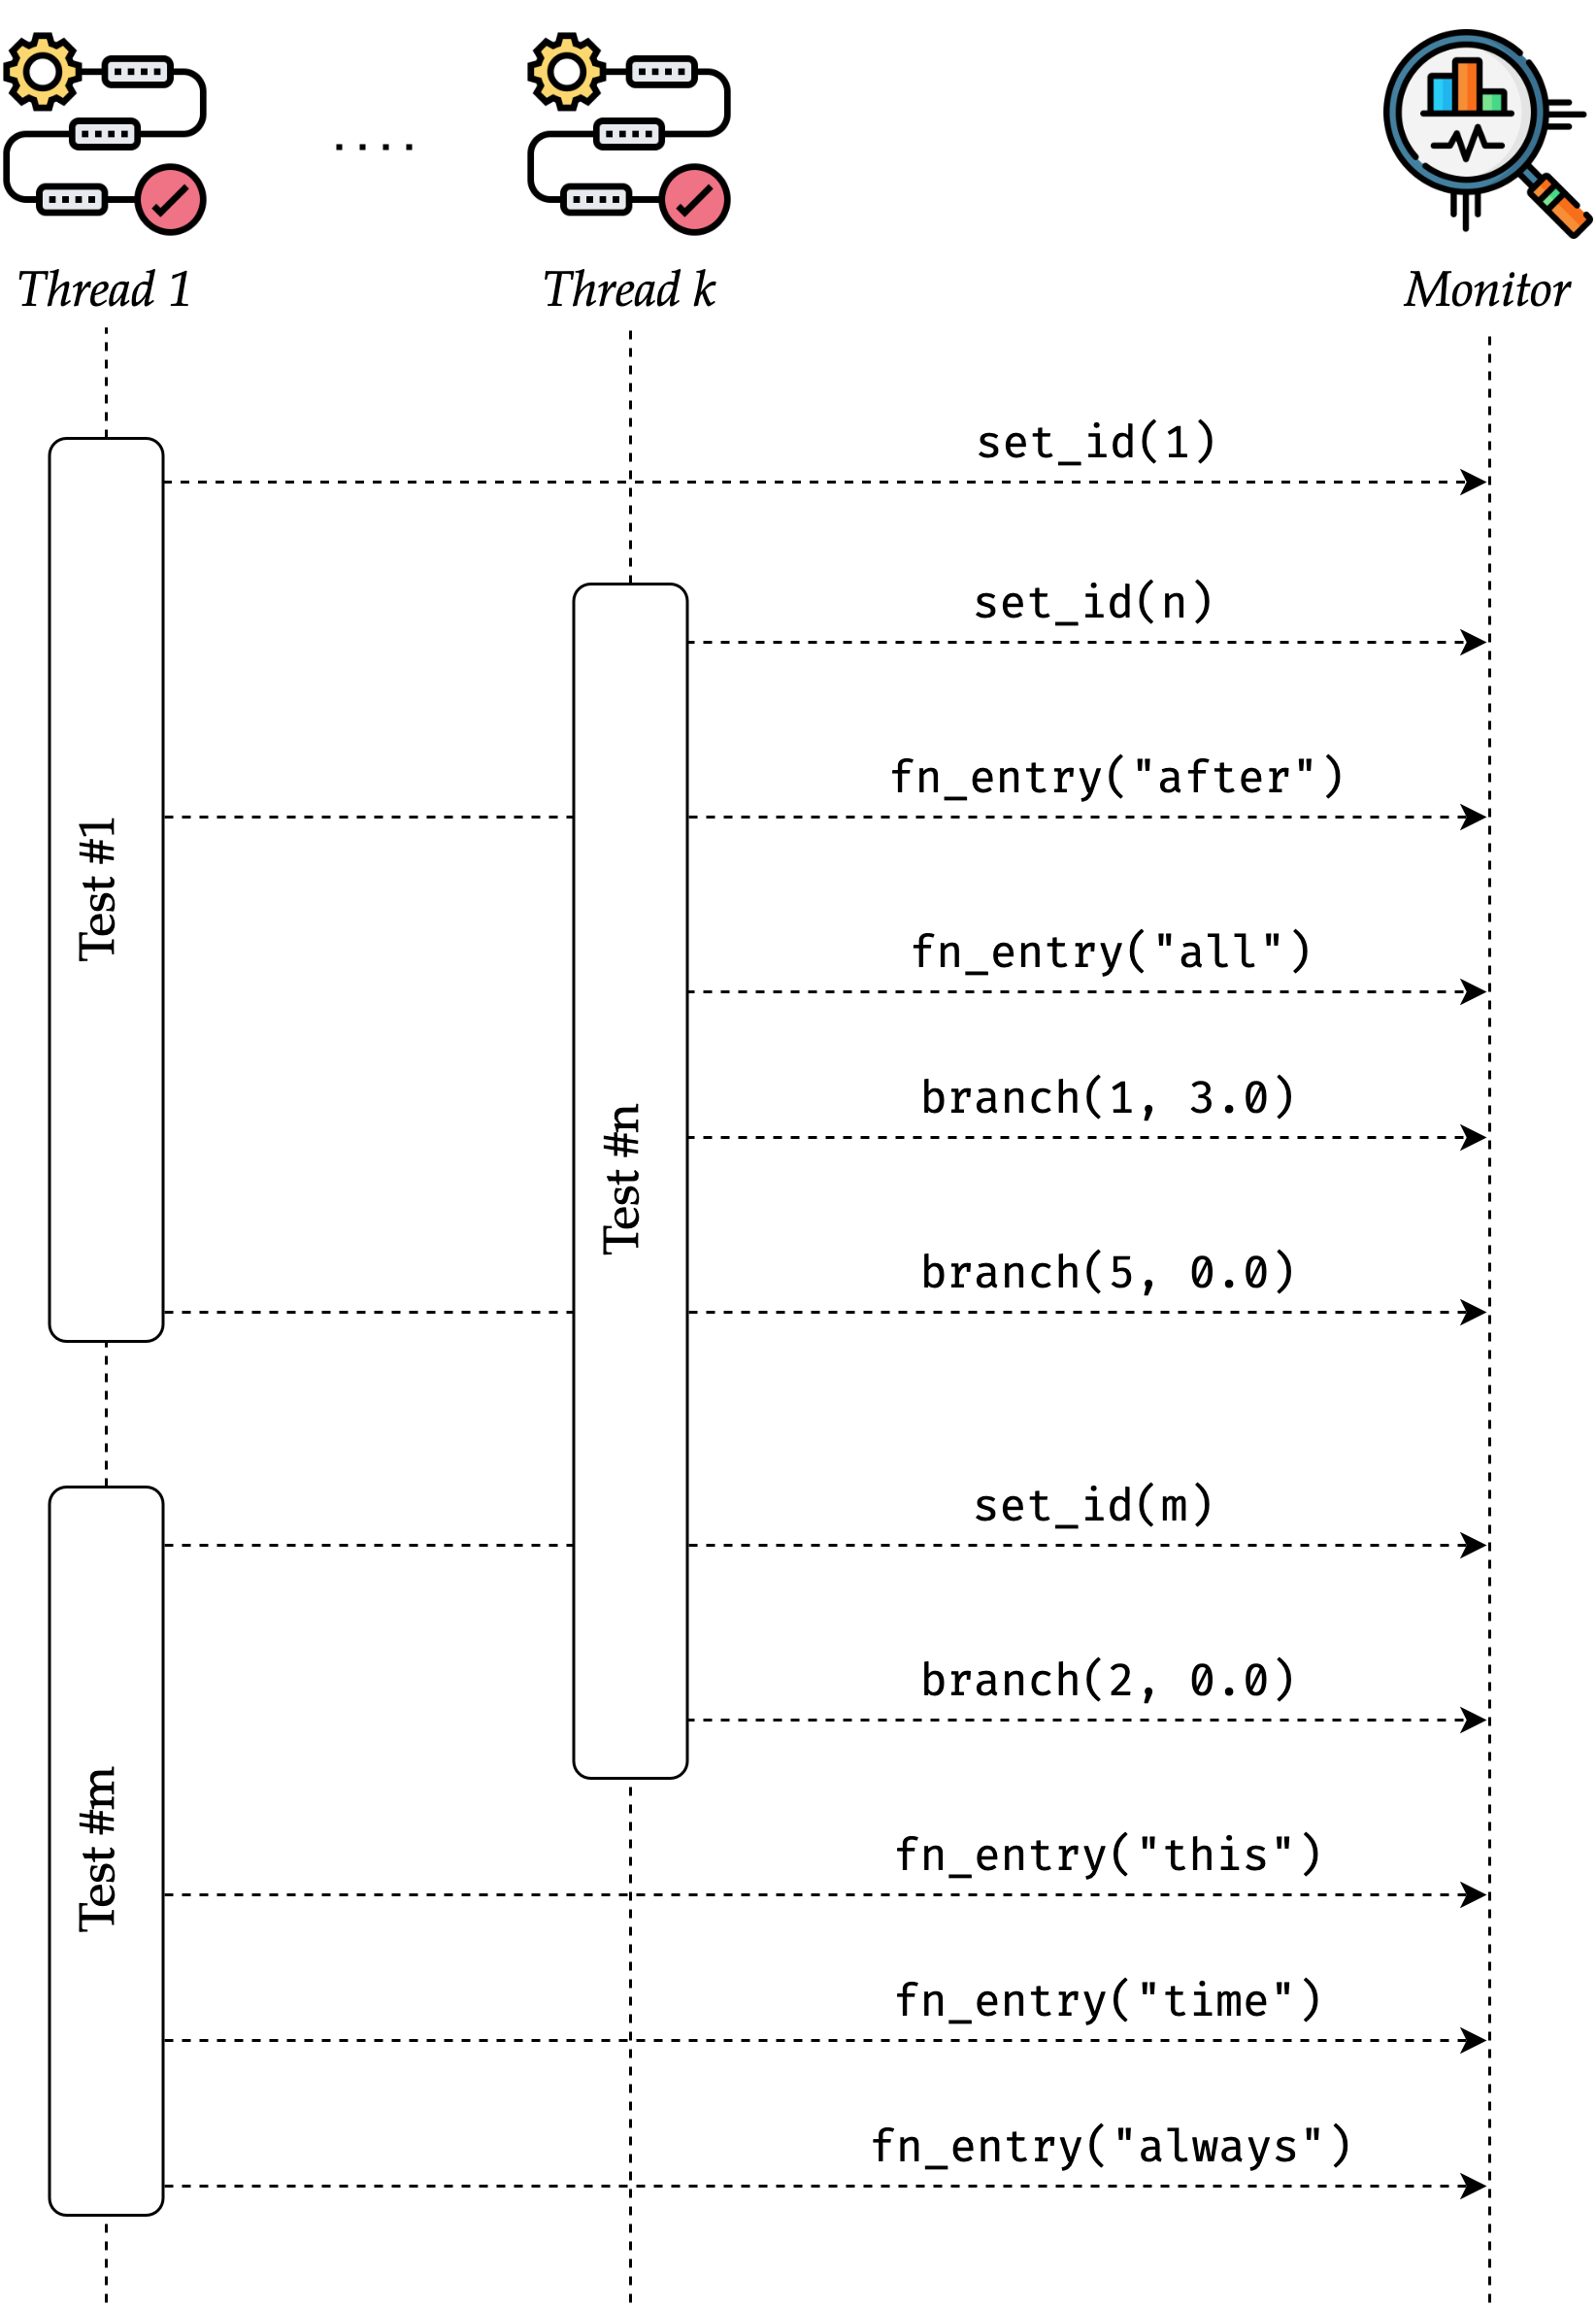
\includegraphics[width=\textwidth]{sequence-diagram/test-execution}
\label{fig:test-execution}
\end{figure}

\clearpage
\chapter{Evaluation}
\label{chap:evaluation}
% TODO reword

We provide an empirical study on our search-based tool \tech for automatic test case generation. We start by our reserch questions in \Cref{sec:research-questions}. Thereafter, we define the criteria for selecting case subjects for evaluation and present our case study in \Cref{sec:case-study-subjects} and explain the environment setup we used in \Cref{sec:environment-setup}. In \Cref{sec:results} we present the results and discuss them in \Cref{sec:discussion}. Finally, we conclude this chapter with a discussion of the threats to validity in \Cref{sec:threats-to-validity}.


\section{Research Questions}
\label{sec:research-questions}
% TODO reword
We now define questions that guide our evaluation. To determine how well our search-based approach performs with respect to code coverage and program crash detection, a set of experiments shall be conducted on a set of open-source Rust programs. As there is already another tool available, namely \textsc{KLEE}, which exploits \ac{DSE} and can also generate tests for Rust, we shall use it in the experiments and compare the results. \textsc{KLEE}-generated tests do not depend on the tool itself and can be executed outside of it the usual way. This opens the possibility to compute a source-based code coverage available in the Rust compiler for both tools. The experiments should answer the following questions:

%Symbolic execution often has problems constructing nice test suites with complex types, which is why this technique is rather applied to find bugs in a \sut, than generate tests with high coverage. Seach-based approach do the opposite, they are good at generating tests with high coverage, but are not as good at finding bugs as they do not make use of test oracles~\cite{Fraser2013}.

\begin{enumerate}[start=1, label={\bfseries RQ\arabic*:}]
    \item How does the \ga of \tech compare to a random search?
    \item What are the characteristics of the generated tests?
    %\item How many coverage goals does \tech cover?
    % Compare coverage and length of tests

    %\item Does the \ac{GA} of \tech achieve a better coverage than random search?
    %\item Does \tech generate less and shorter test cases than random search?
    \item Does \tech improve the coverage of manually written tests in the case study subjects?
    %\item Does \tech achieve a higher code coverage than the \ac{DSE}-based \textsc{KLEE}?
    %\item How do the covered targets of \tech and \textsc{KLEE} differ?
\end{enumerate}

\section{Case Study Subjects}
\label{sec:case-study-subjects}
For the evaluation, we randomly chose \benchnum open-source crates from the Cargo's crate registry. This results in a total of~\methodsnum functions and \branches \mir-level branches.

\todo{Anzahl der \mir-Level Branches berechnen}
\begin{table}[]
\begin{tabular*}{\textwidth}{l @{\extracolsep{\fill}} rrrr}
\hline
\textbf{Case Study} & \textbf{Version} & \textbf{LOC} & \textbf{Functions} & \textbf{Branches} \\
\hline
gamie & 0.7.0 & 328 & 116 &  \\
Pleco & 0.5.0 & 6126 & 1188 &  \\
time & 0.3.7 & 5123 & 1158 &  \\
url & 2.2.2 & 8822 & 529 &  \\
fixed & 1.12.0 & 3604 & 370 &  \\
ibig & 0.3.4 & 4859 & 930 &  \\
nom & 7.1.0 & 3681 & 1375 &  \\
trying & 0.1.0 & 408 & 104 &  \\
rstar & 0.9.2 & 1085 & 330 &  \\
PriorityQueue & 1.2.1 & 1173 & 361 &  \\
\hline
$\sum$ &  & \loc & \methodsnum & \branches \\
\hline
\end{tabular*}
\caption{\label{tab:properties-of-case-study-subjects}Number of lines of code, functions, and \mir-level branches in the case study subjects}
\end{table}
% TODO reword
The libraries were chosen with respect to their testability. For experiments, it is necessary that the units are testable without complex interactions with external resources (e.g., databases, networks and filesystem) and are not multi-threaded. In fact, each experiment should be run in an independent way, and there might be issues if automatically generated test cases do not properly de-allocate resources. Notice that this is a problem common to practically all automated testing techniques in the literature. We also ignored crates that used unsafe or native features such as FFIs. \Cref{tab:properties-of-case-study-subjects} summarizes the properties of these case study subjects in terms of the number of functions, branches, and lines of code. We calculated these metrics using Mozilla's \emph{rust-code-analysis} tool~\cite{Ardito2020}. By \emph{functions} is meant the total number of associative functions, loose functions, and closures. \emph{LOC} the number of logical lines, i.e. statements, in the respective crate as specified by the \emph{LLOC} metric in rust-code-analysis. The tool does not yet support the calculation of the number of branches for Rust, which is why we calculated this metric during the \mir analysis of the case study subjects. The \emph{Branches} column shows the number of branching edges within the \mir of the respective crate.

\section{Setup}
\label{sec:environment-setup}
% TODO reword (Whole Testsuite generation)
As witnessed in \Cref{sec:search-operators}, search algorithms are influenced by a great number of parameters. For many of these there are best practices. We chose many of them based on the experience of other search-based tools like \textsc{EvoSuite}~\cite{Fraser_2011a} and \textsc{Pynguin}~\cite{Lukasczyk2020}. Altough longer test cases are better in general, we limited the length of test cases to $L = 80$ because we experienced this to be a suitable length at which the test case execution does not take too long, altough the initial test cases are generated with only $10$ statements each. The population size for the \ac{GA} was chosen to be $80$.

Search algorithms are often compared in terms of the number of fitness evaluations or generated chromosome samples. That is, the algorithms used in the evaluation have the same budget of generated chromosomes and the performance of the algorithms is compared using the code coverage of test cases that remain after the algorithms have used up the budget. This is what we use to compare \tech with random search. As discussed by Ali et al.~\cite{Ali2010}, a search algorithm should always be compared against at least random search in order to check that the algorithm is not simply successful because the search problem is easy. For evaluation, we have included the option of a random search, which generates random test cases in a manner similar to the initial population in the genetic algorithm of \tech, altough it does not apply optimizations like recombination and mutation. It also exploits an archive and stores test cases that execute previously uncovered branches in a \sut. Random search uses the same parameters for maximum test length, population size, and any probabilities as are set for \tech. The intuition is that the \ac{GA} of \tech will at least provide better test cases in terms of code coverage, since the basis for generation is the same. %but the \ac{GA} of \tech has a lead.
The representations of our genetic algorithm and random search are constructed similarly (e.g., a chromosome is a single test in both cases); thus, such a comparison is a reasonable budget metric. This means that the search is performed until $k$ generated test cases have been executed as part of the fitness evaluations. In our experiments, we chose $k = \budget$. The stopping condition applies for both algorithms.

To measure the performance of the algorithms, the so-called \emph{instrument-coverage} of the Rust compiler is used when evaluating the generated test cases. Rust actually supports two types of coverage. For one, the \emph{gcov}, which uses the debug information to map from LLVM \ac{IR} to source code. In this case, the LLVM \ac{IR} is instrumented to count the executed instructions. However, since LLVM does not know anything about Rust's code structure, a lot of details are lost, and the measured coverage is only an approximation of the actual coverage, which is only moderately good. On the other hand, the newer versions of the Rust compiler support source code-based coverage, also called \emph{instrument-coverage}. Here, the \mir of a \sut is instrumented directly before being converted to the LLVM \ac{IR}. Since the \mir is a mapping between source code and the \cfg of a program, even places like short-circuited conditionals, closures, and match guards can be accurately mapped.

In order to use the instrument-coverage~\footnote{\url{http://web.archive.org/web/20220506220542/https://doc.rust-lang.org/rustc/instrument-coverage.html}} the crate tested must be compiled with the corresponding flag \texttt{-C instrument-coverage}. This requires a \emph{profiler runtime}, which is already included in the \emph{nightly} compiler. Thus, a corresponding \sut can be built with \raggedright\texttt{RUSTFLAGS="-C instrument-coverage" cargo +nightly build}. When the built program or test is executed, LLVM generates corresponding coverage (\emph{profraw}) files, which after post-processing contain the line as well as branch coverage per source file of the \sut. For each of the two algorithms, we compare the line and branch coverage, as well as the length and number of generated tests. Since both tools, random search and \tech, generate tests in source code form, they can be compiled along with the \sut and their source code-based coverage can be directly compared.

From the perspective of the instrument-coverage, unit tests are usual code whose coverage is also measured, i.e., which statements and branches (if any) of a test were executed. However, based on this behavior, the overall coverage in our experiments would be heavily affected by the number and length of the generated tests. For instance, assume a crate with two functions \emph{a} and \emph{b} that do not contain any branches and execute entirely upon an invocation, with $\left|a\right| = 5$ and $\left|b\right| = 5$. Then, a test that only consists of a single invocation of function~\emph{a}, executes 6 statements out of 11 available, i.e., has a coverage of about 55\%. Another test that invokes function~\emph{b} 50 times without a loop, i.e., consists of 50 statements, executes 55 statements out of 60 available and thus, has a coverage of nearly 92\%. Even though both tests effectively touch exactly a half of the crate's code, their computed coverage is higher and even differs based on their length. To mitigate this issue, we exploit the \emph{no\_coverage}~\footnote{\url{https://web.archive.org/web/20220520122617/https://doc.rust-lang.org/nightly/unstable-book/language-features/no-coverage.html}} attribute and annotate the generated test cases with it. The attribute selectively disables coverage instrumentation in the annotated function. Thus, we only compute the coverage of the productive code.

Rust does not incorporate the concept of exceptions; instead, the language employs the \texttt{Result} type for recoverable errors and crashes, or panics, on unrecoverable errors. \texttt{Result} is an enum and given an instance of it, we can check whether its wraps a true value or some error instance.
The tests automatically generated by \tech can fail for various reasons, e.g., because the arguments generated for a function call result in an integer overflow, a function calls \texttt{panic!()} explicitly under some condition, or a statement tries to unwrap an erroneous \texttt{Result}. Unfortunately, we cannot compute the code coverage with instrument-coverage for tests that fail. Since we explicitly try to cover all branches, we want to have those test cases in the final test suite and compute their coverage, too. Therefore, we exploit Rust's \emph{should\_panic} attribute for failing tests, which inverts the result of a test, i.e., a test passes if it panics, otherwise it fails.



\section{Results}
\label{sec:results}
% TODO reword
In the following we analyse the benchmark results in order to answer our research questions and test our hypotheses. \tech, as other search-based testing tools, relies on randomized algorithms, which are inherently affected by chance. Running a randomized algorithm twice will most likely produce different results. It is essential to use rigorous statistical methods to properly analyze the performance of randomized algorithms when we need to compare two or more of them. In this work, we follow the guidelines described by Arcuri and Briand~\cite{Arcuri2011}. Since comparisons with simpler alternatives (at a very minimimum random search) is a necessity when one proposes a novel randomized algorithm or addresses a new software engineering problem~\cite{Ali2010}, statistical testing should be part of the according work, which reports such empirical study. For each of the \benchnum crates, we ran \tech against the random search to compare their achieved code coverage. Each experiment comparison was repeated \runs times with different seeds for the random number generator.  %(~\cite{Arcuri2011} schlägt mindestens $1000$ vor, bei begründet langer Ausführungszeit kann es auch weniger sein) .

% TODO reword
In particular, when branch coverage values were compared, statistical difference has been measured with the Mann-Whitney U test. To quantify the improvement in a standadized way, we used the unparameterized Vargha-Delaney~$\hat{A}_{12}$ effect size test. In our context, the $\hat{A}_{12}$ is an estimation of the probability that, if we run \tech, we will obtain better coverage than running the random search strategy. When two randomized algorithms are equivalent, then $\hat{A}_{12} = 0.5$. A high value $\hat{A}_{12} = 1$ means that, in \emph{all} of the \runs runs of \tech, we obtained coverage values higher than the ones obtained in \emph{all} of the \runs runs of the random search strategy.

\subsection{\tech vs Random Test Generation}
\begin{figure}[ht]
\caption{\label{fig:results-ru-rs-coverage}Branch coverage results per crate}
\centering
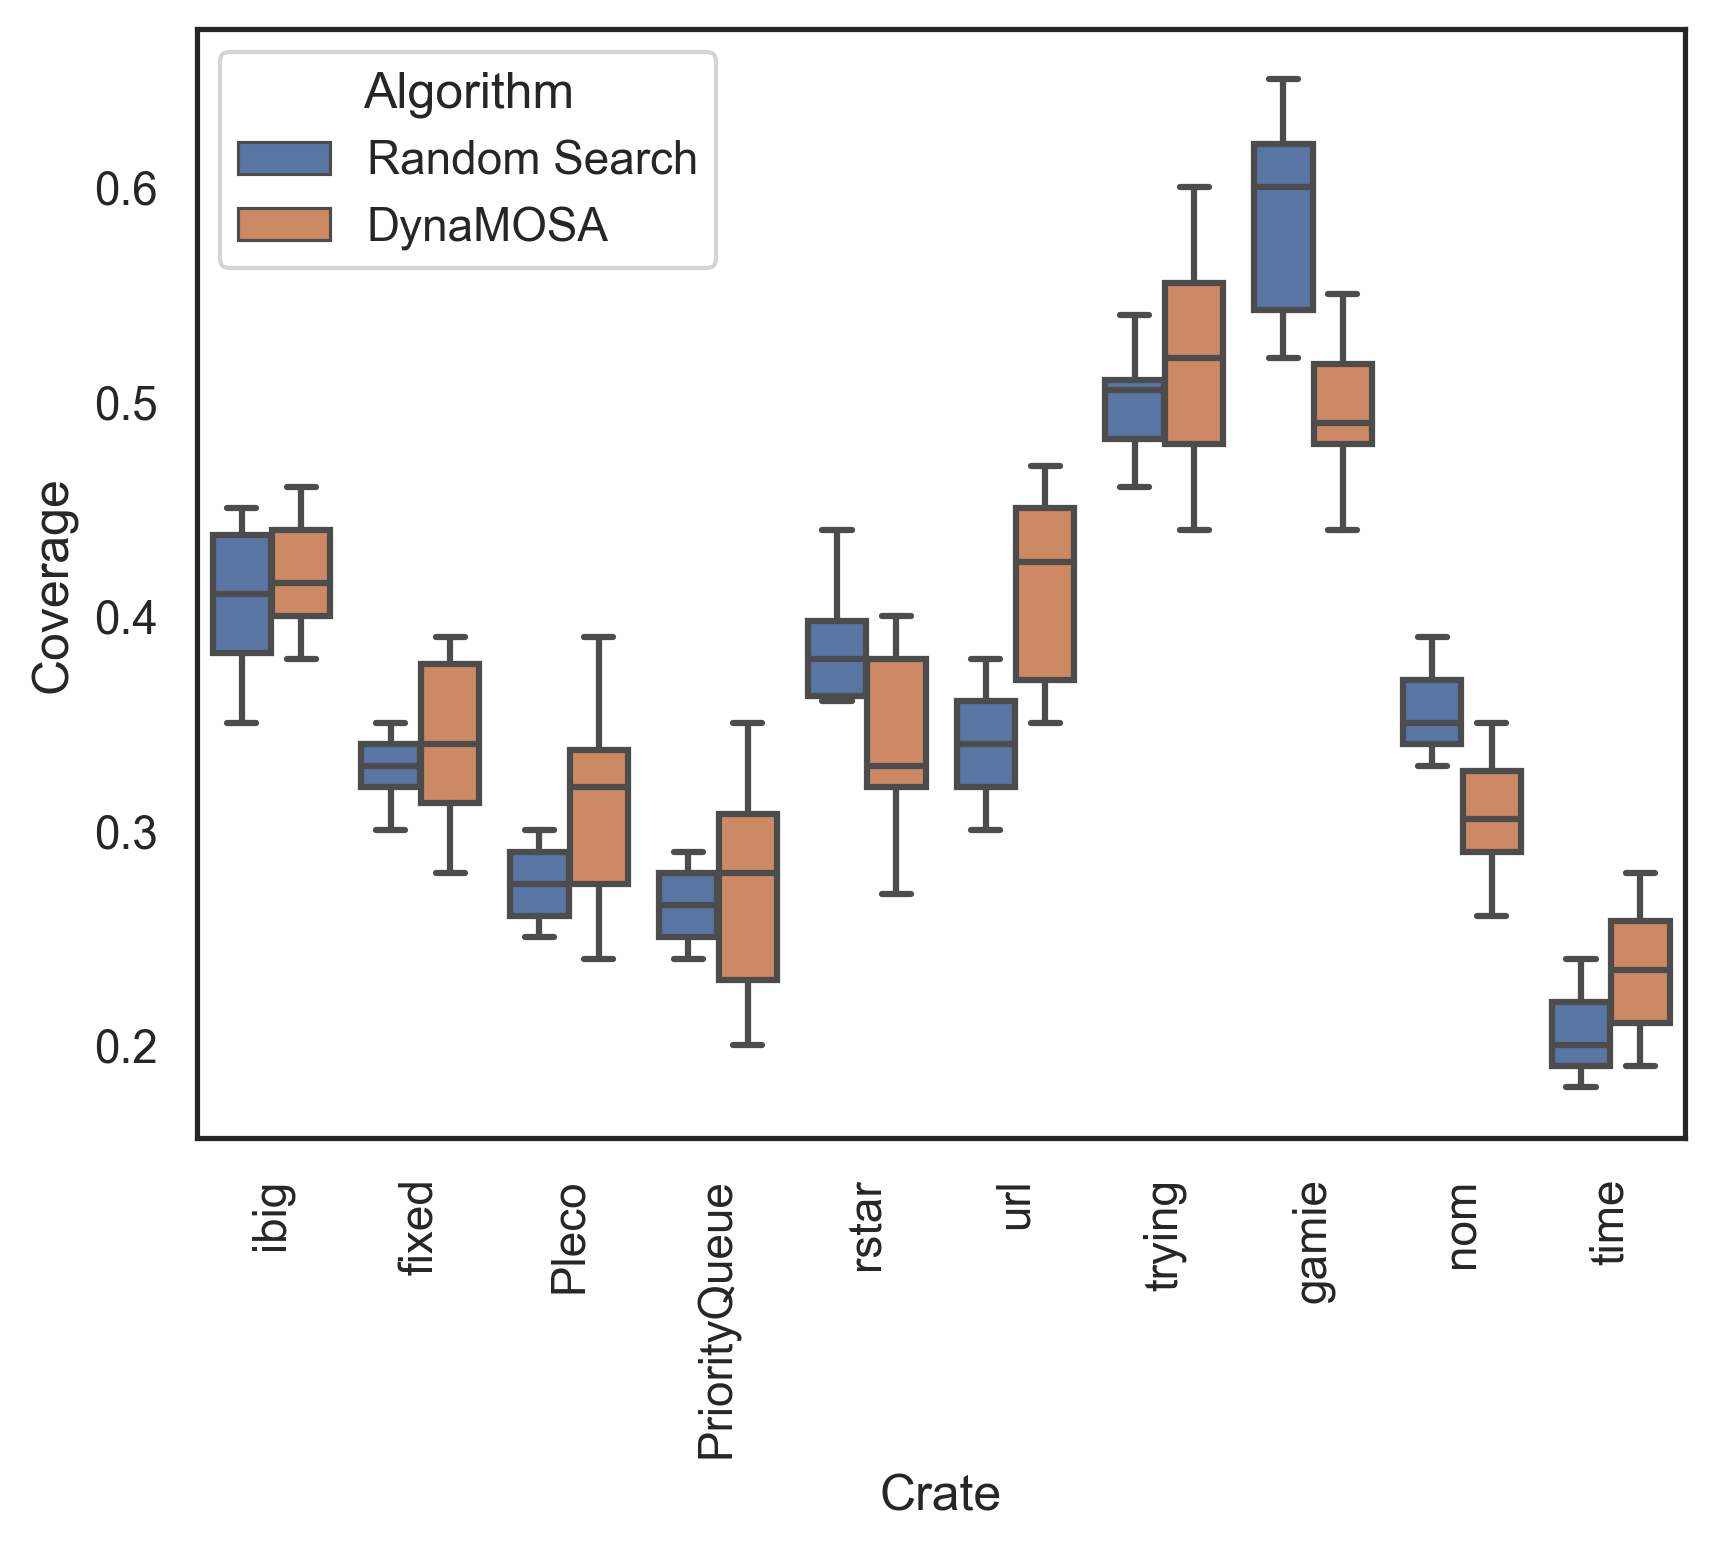
\includegraphics[width=\textwidth]{coverage}
\end{figure}

The box-plot in~\Cref{fig:results-ru-rs-coverage} compares the actual obtained branch coverage values over \runs runs of \tech and random search. In total, the coverage improvement of \tech ranged up to 7\% than that of random search. Calculated on all the crates we used in the case study, \tech obtained an average coverage of 38\%, whereas random search obtained 36\%.

\Cref{fig:results-ru-rs-coverage} shows the average branch coverage obtained for each of the \benchnum crates. The results in~\Cref{tab:results-ru-rs-coverage} present a hopeful perspective.

% RQ 1 answer
\begin{tcolorbox}
\textbf{Summary (RQ1):} \tech achieves a comparable coverage to random random test generation. For some crates, it achieves a significantly better coverage.
\end{tcolorbox}

\Cref{tab:results-ru-rs-coverage} shows for the coverage comparisons which $\hat{A}_{12}$ values we obtained for the crates in the case study. For instance, for \emph{gamie}, the $\hat{A}_{12}$ value of 0.8 means that \tech obtained a higher coverage in 80\% of the cases. The table also provides results of the Mann-Whitney U test that we conducted per crate with the H0 hypothesis that the two algorithms evaluated do not differ in terms of achieved coverage.
We obtained p-values lower than the traditional $\alpha = 0.05$ for 7 crates, which means that the coverage differences over \runs executions are statistically significant. However, \tech could only achieve better coverage in 5 of the 7 crates. However, Arcuri~\cite{Arcuri2011} suggests that the significance value $\alpha$ is much less of importance in the context of \ac{SBST}; one should state all the results regardless of their significance and let the reader decide for himself to what extent a particular algorithm suits their needs. Statistical evaluation and practical, ``felt'' results can differ greatly for randomized algorithms.

% For this purpose, we take the unparameterized Vargha and Deleney's $\hat{A}_{12}$ measure of effect size. Its use for randomized algorithms in software engineering was justified in~\cite{Leech2002} and an example of its use in the context of software engineering with randomized algorithms is shown in~\cite{Poulding2010}.

% TODO reword
In theory, a t-test would be possible, too; however, it requires a normal distribution of the experiment results, which is not given for search-based test generation in general. Furthermore, we cannot determine the true mean and variance values since the search could run for an infinite period of time continuously generating better results, provided that the 100\% coverage is not reached. Practically, the search is limited by the computational and memory capacity of the machine which the experiments run on, but it is only an artificial limit.

Both algorithms only achieve moderately high coverage up to 59\%. The main reason is that the analysis of the possible function invocations and types is still limited. For instance, we cannot execute most of generic traits or derived trait implementations (e.g., \texttt{\#[derive(Debug)]}) since the derived traits either require some advanced generics analysis, too, or parameters that we cannot instantiate. Derived traits are generated  In case of \texttt{Debug}, which is one of the most often derived traits, its only method \texttt{fmt} requires an argument of type \texttt{std::fmt::Formatter} that we cannot create. Usually it is created automatically by macros when we print its implementing type, e.g., %\texttt{print!("\string{\string}", some_var)}.
With this limitations, it is not possible to achieve a 100\% coverage for non-trivial traits.

However, since the limitations apply to both algorithms the same, the results are still comparable. Even though \tech achieves for some crates significantly better results, in practice, it does not outperform random search by much. Moreover, random search yielded better results for three of the experiment subjects. The issue is that even with the real crates, the search problem is still easy enough, especially since our implementation cannot extract complex parts of a \sut. \ac{DynaMOSA}, the \ac{GA} which \tech exploit, is especially tailored to highly nested control dependency structures of object-oriented programs that can be explored iteratively using the approach level guidance. However, Rust is not a typical object-oriented language, and the case study subjects feature \cdgs with an average depth of about $1.1$ \textbf{TODO CDG Eigenschaften der in einer Tabelle aufführen}. That is, \tech cannot develop its full potential and employ guided search as it is mainly dependent on branch distance, which, as explained in~\Cref{sec:fitness-function}, can only be $0$ or $1$ for non-numerical data. Thus, \tech degenerates to random search, too. In fact, for some cases it is even worse than that. Whereas random search continues to generate new test cases independently and hits more uncovered targets faster, the genetic algorithm tries to surgically improve test cases that often cannot be improved anyway due to shallow control dependecies within the functions invoked in those tests.

\todo{Show an example function from a crate and its CDG.}

\begin{table}[]
  \begin{tabular*}{\textwidth}{l @{\extracolsep{\fill}} rrrr}
  \hline
  \textbf{Case Study} & Random Search & \tech & \textbf{$\hat{A}_{12}$} & p-value \\
  \hline
  gamie & 0.59 & 0.49 & \textbf{0.04} & \textbf{< 0.001} \\
  Pleco & 0.27 & 0.31 & \textbf{0.76} & \textbf{< 0.001} \\
  time & 0.21 & 0.24 & \textbf{0.8} & \textbf{< 0.001} \\
  url & 0.34 & 0.41 & \textbf{0.90} & \textbf{< 0.001} \\
  fixed & 0.33 & 0.34 & 0.61 & 0.11 \\
  ibig & 0.41 & 0.42 & 0.59 & 0.23 \\
  nom & 0.36 & 0.31 & \textbf{0.08} & \textbf{< 0.001} \\
  trying & 0.5 & 0.52 & 0.61 & 0.15 \\
  rstar & 0.38 & 0.34 & \textbf{0.19} & \textbf{< 0.001} \\
  PriorityQueue & 0.27 & \textbf{0.27} & 0.56 & \textbf{< 0.001} \\
  \hline
  Average & 0.36 & 0.38 & 0.59 & \\
  \hline
  \end{tabular*}
% TODO reword caption
\caption{\label{tab:results-ru-rs-coverage}For each crate, the table reports the average branch coverage obtained by random search and \tech. Effect sizes and p-values are in bold when the p-values are lower than 0.05}
\end{table}

\todo{How many of the practically possible target do we actually cover?}

Since we still want to analyze how the effect impact of the \ga of \tech despite the implementation limitations and the features of the case study subjects from~\Cref{tab:properties-of-case-study-subjects}, we constructed a toy crate which does not make use of advanced language features and is non-trivial at the same time. In the following, some of the \textsc{ToyCrate}'s functions are presented.

\todo{Ein paar Beispielfunktionen aus ToyCrate + Ergebnisse der Coverage.}

\subsection{Characteristics of generated tests}
In this section, we analyse the impact of the selected algorithm on the length of the generated test cases and try to answer RQ2, again using the per-crate Mann-Whitney U p-values and $\hat{A}_{12}$ effect sizes. \Cref{fig:results-ru-rs-length} illustrates the average test lengths of the tests produced by random search and \tech over the \runs runs. For \tech, we observe a positive effect on most of the crates. For Pleco and  trying, random search produces shorter test cases on average, though. For other crates, the length of the tests is similar. \Cref{tab:results-ru-rs-length}
\subsection{\tech vs Random Test Generation}
\begin{figure}[ht]
\caption{\label{fig:results-ru-rs-length}Average test case length per crate}
\centering
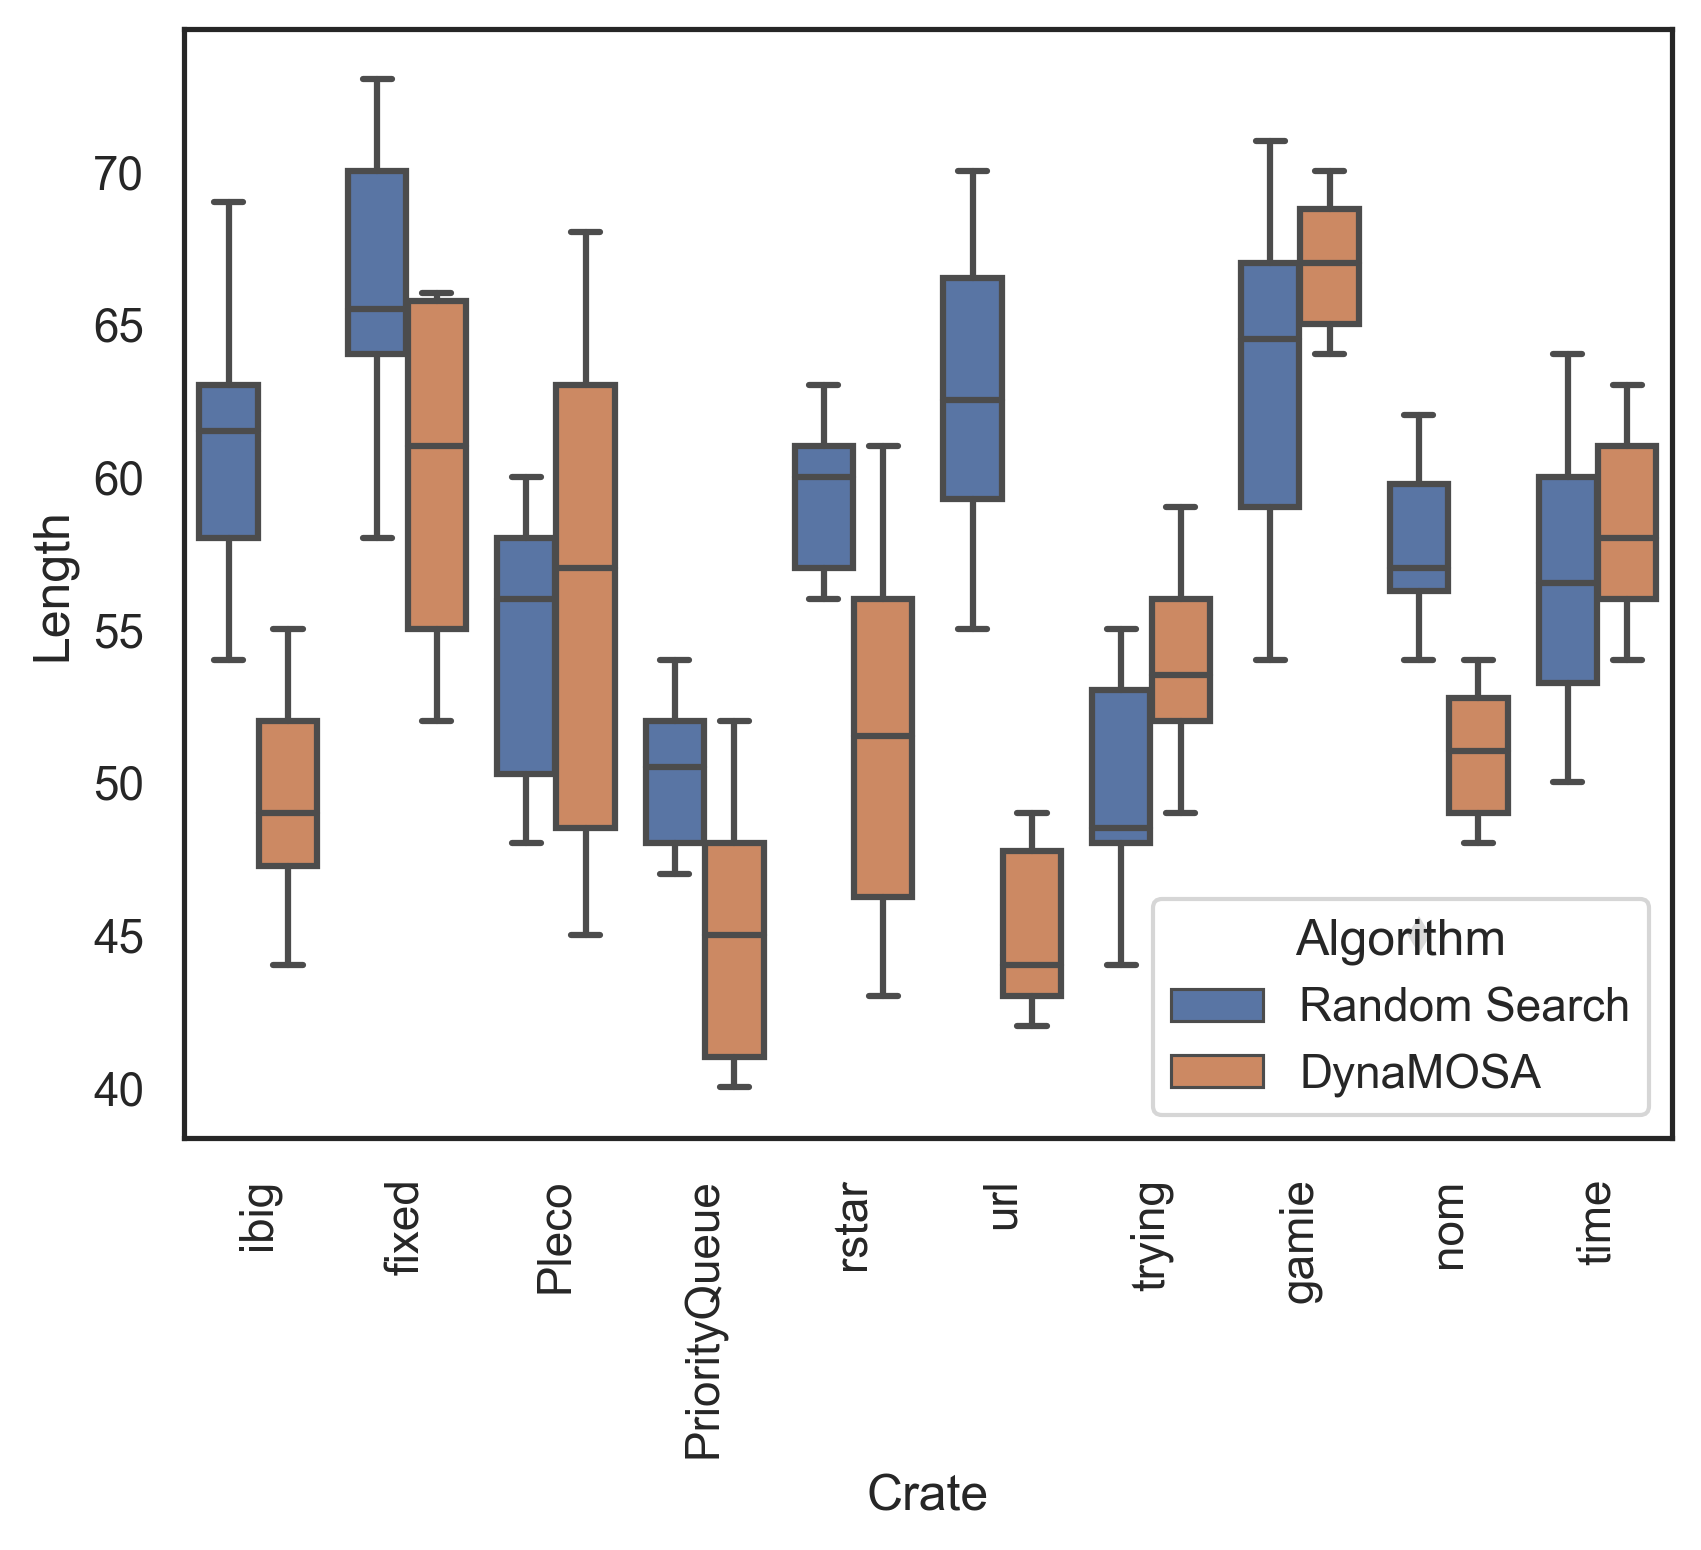
\includegraphics[width=\textwidth]{length}
\end{figure}

\textbf{continue.}
%\csvautotabular{experiments/coverage.csv}

\begin{table}[]
  \begin{tabular*}{\textwidth}{l @{\extracolsep{\fill}} rrrr}
  \hline
  \textbf{Case Study} & Random Search & \tech & \textbf{$\hat{A}_{12}$} & p-value \\
  \hline
  gamie & 63.1 & 67.1 & \textbf{0.27} & \textbf{0.003} \\
  Pleco & 54.7 & 56.1 & 0.44 & 0.39 \\
  time & 56.6 & 58.4 & 0.37 & 0.075 \\
  url & 62.5 & 44.8 & \textbf{1.0} & \textbf{< 0.001} \\
  fixed & 66.3 & 60.2 & \textbf{0.79} & \textbf{< 0.001} \\
  ibig & 61.1 & 49.5 & \textbf{0.99} & \textbf{< 0.001} \\
  nom & 57.6 & 50.9 & \textbf{95.8} & \textbf{< 0.001} \\
  trying & 49.6 & 54.0 & \textbf{0.17} & \textbf{< 0.001} \\
  rstar & 59.2 & 51.6 & \textbf{0.89} & \textbf{< 0.001} \\
  PriorityQueue & 50.4 & 44.9 & \textbf{0.89} & \textbf{< 0.001} \\
  \hline
  Average & 58.2 & 53.8 & 0.67 & \\
  \hline
  \end{tabular*}
% TODO reword caption
\caption{\label{tab:results-ru-rs-length}For each crate, the table reports the average test case length obtained by random search and \tech. Effect sizes and p-values are in bold when the p-values are lower than 0.05}
\end{table}


% RQ 2 answer
\begin{tcolorbox}
\textbf{Summary (RQ2):} \tech generates shorter test cases for most of the case study subjects.
\end{tcolorbox}

%\subsection{Failing Tests}
%Figure ... lists the failures found in each of the case study subject by \tech.

\subsection{Manually Written Tests}
\begin{tcolorbox}
\textbf{Summary (RQ2):} \todo{To be done yet.}
\end{tcolorbox}

\section{Threats to Validity}
\label{sec:threats-to-validity}
%\subsection*{Internal Validity}

\subsection*{External Validity}
% TODO reword
We used \benchnum open-source crates for our evaluation. They are small and, above all, have as few dependencies as possible, i.e., they stay self-contained. The crates do not interact with the environment, e.g., by means of I/O, nor do they use some sort of parallelism. Furthermore, the number of subjects and their intention is not diverse enough, so the results may not generalize to all Rust programs.

\subsection*{Construct Validity}
% TODO reword
Strictly speaking, some of the generated tests may not fall into the category of unit tests, as our approach cannot mock dependencies and instead generates real instances regardless of their origin and complexity. The testing frameworks for Rust are still very limited in their flexibility because mocks, like so many other things in Rust, are created using macros at compile time. Also, they can mostly only mock traits and no structs or enums. Furthermore, with our approach, we cannot measure fault finding capability of the generated tests as our tool does not employ assertions, which is explicitly out of scope of this work. Finally, our approach exploits instrumentation and analysis of \mir, which is unstable and is subject to silent and breaking changes. That is, applying \tech on Rust programs with future version of the Rust compiler might require some changes of the instrumentation technique used.

\section{Conclusion}
\label{sec:discussion}
\todo{Conlcusion.}


\clearpage
\chapter{Future Work}
\label{chap:future-work}
% TODO reword
Solving a research problem almost always leads to new problems and further open questions. In this final section of the thesis, we want to discuss a few such questions that arose during the work on the thesis. We leave them as future work because they would blast the scope of this work.

We already stated in the evaluation that the whole process of generating tests for Rust with \tech is relatively slow and cannot be applied easily to all crates of any size out in the wild. The execution time is tied to the execution of the Rust compiler and I/O operations, which means that the cost of the runtime of the generated tests themselves is not the bottleneck in general. At this point, cache optimizations could be made or the way \sut is instrumented and tests are executed could be adjusted. Furthermore, the generated tests contain a lot of unnecessary statements even though \tech eliminates some of them during search, which lead to the running, but more importantly comprehension overhead of a humble developer who would have to deal with them since the tests do not automatically employ assertions. This leads us to the other aspect of test generation: \tech does not generate real test cases, but only program executions. A test oracle, which determines whether the result of an execution is correct and meets the expectations, is missing. Some test generation tools, such as \textsc{EvoSuite}, can automatically incorporate assertions, for example by using the recorded behavior of \sut for regression testing. In the future, a mechanism for automatically generated oracles could also be provided in \tech.

Another aspect of test generation is the scope of the test cases. Unit testing, as the name suggests, refers to individual units. Traditionally, complex dependencies are replaced by mocks in unit tests, e.g., a database connection. As far as possible, \tech exploits real data types, even if they originate in other units, which makes some test more integration than unit tests. Rust's ecosystem already offers many mock libraries, but unlike Java, they do not rely on runtime reflection, but on Rust's strong macro system and generate mocks at compile time. It would be interesting to extend \tech's search-based algorithm with functional mocks to achieve potentially better coverage, such as Arcuri et al.~\cite{Arcuri2017} do for \textsc{EvoSuite}.

One further significant facet to consider is the execution environment. Real and complex software often interacts with its environment, for example by making I/O calls to the file system or establishing \ac{TCP} connections. Lack of handling of the execution environment the \sut lives within is still one of the open problems in \ac{SBST}~\cite{McMinn2011} and poses many problems since running a program with automatically and randomly generated input data can have unpredictable effects, such as, for example, hard disk erasure. To avoid unwanted side effects, \textsc{EvoSuite}~\cite{Fraser2013a} exploits the Java Security Manager to prohibit most possible interactions of a \sut with its environment. \textsc{KLEE}~\cite{cadar2008klee} takes a different approach and redirects concrete calls, such as file system's \texttt{open()} and \texttt{read()}, to \emph{models} that understand the semantics of the desired action well enough to generate the required constraints. A similar approach could be applied to Rust programs, i.e., transform the \mir of a \sut on-the-fly during the compilation in such way that environment interaction become harmless or even mock them.

As for seeding the initial population of test cases, there exist futher techniques that could be applied and evaluated for Rust, such as incorporating manually written unit tests. Often programs already contain test cases that do not cover the entire code but only the regular execution flow. An approach is to use those tests as part of the initial population to cover edge cases, for instance. However, the existing tests must first be converted into the representation that a \ga uses. This means that they have to be parsed in the case of \tech. Luckily, Rust already provides mature libraries for this purpose, e.g., \emph{syn}~\footnote{\url{https://web.archive.org/web/20220520083112/https://crates.io/crates/syn}}.

Finally, it would be useful to use Rust's compiler analysis for more meaningful tests. \tech is a compiler wrapper and can thus access all compiler internals during the analysis of the \sut. Advanced static analysis of the \sut, such as interprocedural search of the initialization of operands used in conditions, could help generate better tests with higher coverage.


\backmatter% Now we are in the appendix
\appendix
\cleardoublepage
\thispagestyle{empty}
\null\vfill
\noindent\textbf{Eidesstattliche Erklärung:}\\[1.5ex]
Hiermit versichere ich an Eides statt, dass ich diese Bachelorarbeit
selbstständig und ohne Benutzung anderer als der angegebenen Quellen und
Hilfsmittel angefertigt habe und dass alle Ausführungen, die wörtlich oder
sinngemäß übernommen wurden, als solche gekennzeichnet sind, sowie dass ich die
Masterarbeit in gleicher oder ähnlicher Form noch keiner anderen
Prüfungsbehörde vorgelegt habe.\\[1.5cm]
Passau, \today\quad\rule{6cm}{0.1mm}\\
\null\hspace{5cm} {\small Vsevolod Tymofyeyev}

\clearpage
\chapter{Acronyms}
\begin{acronym}
	\acro{SUT}{System Under Test}
	\acro{CUT}{Class Under Test}
	\acro{MUT}{Method Under Test}
	\acro{SMT}{Satisfiability Modulo Theories}
	\acro{GA}{Genetic Algorithm}
	\acro{EA}{Evolutionary Algorithm}
	\acro{MOSA}{Many-Objective Sorting Algorithm}
	\acro{DynaMOSA}{Many-Objective Sorting Algorithm with Dynamic target selection}
	\acro{WS}{Whole Suite}
	\acro{WSA}{Whole Suite with Archive}
	\acro{SBST}{Search-based Software Testing}
	\acro{SBSE}{Search-based Software Engineering}
	\acro{ATP}{Automated Theorem Prover}
	\acro{DSE}{Dynamic Symbolic Execution}
	\acro{IR}{Intermediate Representation}
	\acro{MOA}{Multi- and Many-Objective Algorithm}
	\acro{DDG}{Data Dependence Graph}
	\acro{HIR}{High-level Intermediate Representation}
	\acro{THIR}{Typed HIR}
	\acro{MIR}{Mid-level Intermediate Representation}
	\acro{AST}{Abstract Syntax Tree}
	\acro{CFG}{Control Flow Graph}
	\acro{CDG}{Control Dependence Graph}
	\acro{API}{Application Programming Interface}
	\acro{NSGA-II}{Non-dominated Sorting Genetic Algorithm II}
	\acro{TCP}{Transmission Control Protocol}
	\acro{SSA}{Static Single Assignment}
\end{acronym}

\clearpage
\printbibliography
\end{document}
